\newpage
\section{Flow profiles}\label{app:flow_profiles}
In this appendix the flow profiles that describes the flow from the residential, industrial and brewery and bottling plant used in the simulation is shown. Furthermore, profiles that describes the concentration intake to the WWTP is also included.

The legend in the plots references to the figure \ref{fig:kloakgrid_simplified} shown in chapter \ref{se:system_description}. 


\begin{figure}[H]
\centering
% This file was created by matlab2tikz.
%
%The latest updates can be retrieved from
%  http://www.mathworks.com/matlabcentral/fileexchange/22022-matlab2tikz-matlab2tikz
%where you can also make suggestions and rate matlab2tikz.
%
\definecolor{mycolor1}{rgb}{0.00000,0.44700,0.74100}%
\definecolor{mycolor2}{rgb}{0.85000,0.32500,0.09800}%
\definecolor{mycolor3}{rgb}{0.92900,0.69400,0.12500}%
\definecolor{mycolor4}{rgb}{0.49400,0.18400,0.55600}%
\definecolor{mycolor5}{rgb}{0.46600,0.67400,0.18800}%
%
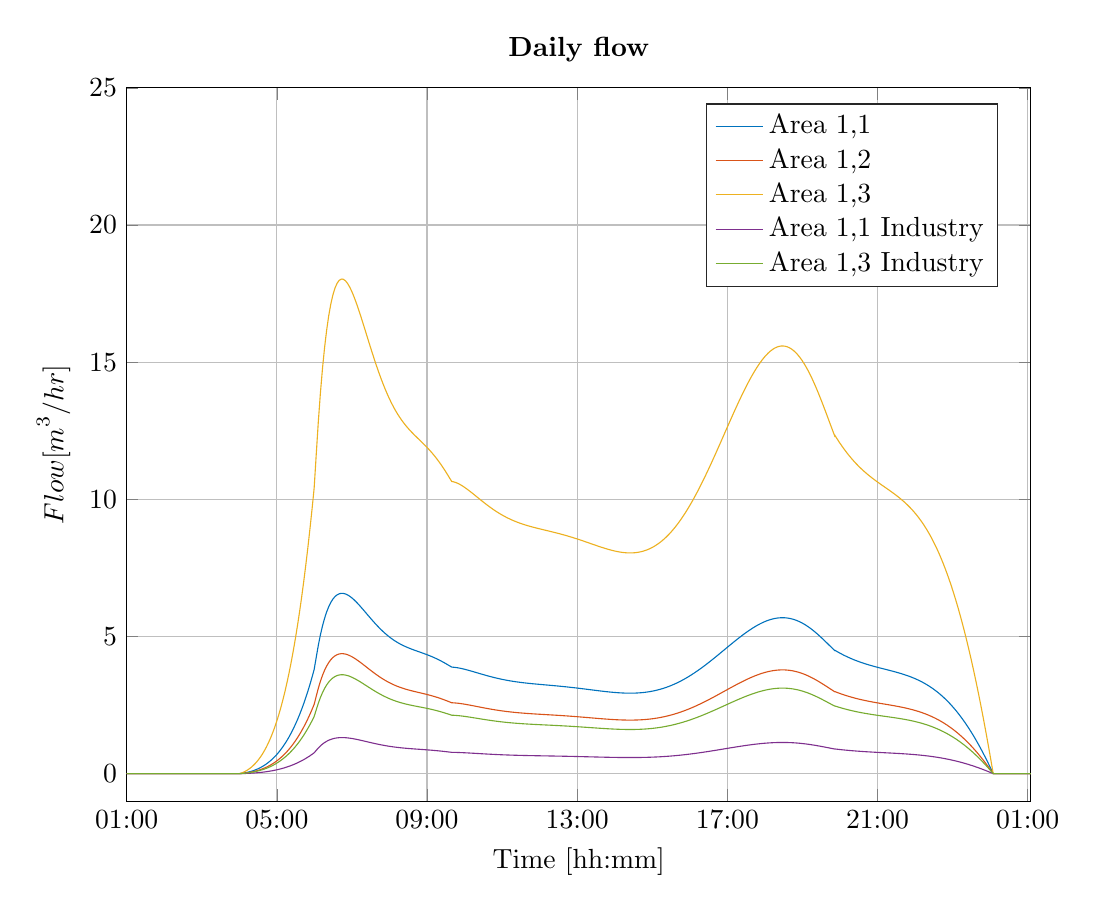
\begin{tikzpicture}

\begin{axis}[%
width=4.521in,
height=3.566in,
at={(0.758in,0.481in)},
scale only axis,
xmin=3600,
xmax=90000,
xtick={3600,17950,32300,46650,61000,75350,89700},
xticklabels={{01:00},{05:00},{09:00},{13:00},{17:00},{21:00},{01:00},{},{},{}},
xlabel={Time [hh:mm]},
scaled x ticks = false,
xmajorgrids,
ymin=-1,
ymax=25,
ylabel={$\text{Flow [m}^\text{3}\text{/hr]}$},
ymajorgrids,
axis background/.style={fill=white},
title style={font=\bfseries},
title={Daily flow},
legend style={at={(0.641,0.721)},anchor=south west,legend cell align=left,align=left,draw=white!15!black}
]
\addplot [color=mycolor1,solid]
  table[row sep=crcr]{%
3599	0\\
3799	0\\
3998	0\\
4197	0\\
4396	0\\
4595	0\\
4794	0\\
4993	0\\
5192	0\\
5391	0\\
5590	0\\
5789	0\\
5988	0\\
6188	0\\
6387	0\\
6586	0\\
6785	0\\
6984	0\\
7183	0\\
7382	0\\
7581	0\\
7780	0\\
7979	0\\
8178	0\\
8377	0\\
8577	0\\
8776	0\\
8975	0\\
9174	0\\
9373	0\\
9572	0\\
9771	0\\
9970	0\\
10169	0\\
10368	0\\
10567	0\\
10766	0\\
10965	0\\
11165	0\\
11364	0\\
11563	0\\
11762	0\\
11961	0\\
12160	0\\
12359	0\\
12558	0\\
12757	0\\
12956	0\\
13155	0\\
13354	0\\
13554	0\\
13753	0\\
13952	0\\
14151	0\\
14350	0\\
14549	0.00710028180255936\\
14748	0.0184228250217605\\
14947	0.0320492223793003\\
15146	0.0482073693016751\\
15345	0.0671355323234623\\
15544	0.0890823640800493\\
15743	0.114306906530896\\
15942	0.143078582413403\\
16142	0.175851135929245\\
16341	0.212588195200944\\
16540	0.253744214191448\\
16739	0.299629869141819\\
16938	0.350565997430973\\
17137	0.406883518354036\\
17336	0.468923342131185\\
17535	0.537036267147258\\
17734	0.611582865421718\\
17933	0.692933356309431\\
18132	0.781467468431938\\
18331	0.877574289839258\\
18531	0.982195922443594\\
18730	1.09469519004965\\
18929	1.21599102593738\\
19128	1.3465082650137\\
19327	1.48668017480407\\
19526	1.63694823493869\\
19725	1.79776190486959\\
19924	1.96957837981796\\
20123	2.15286233495235\\
20322	2.34808565779734\\
20521	2.55572716887281\\
20720	2.77627233056388\\
20920	3.0114231889665\\
21119	3.25932816256334\\
21318	3.52163248137147\\
21517	3.79884505460662\\
21716	4.24535835961483\\
21915	4.68162393830136\\
22114	5.0605303399952\\
22313	5.38652724971494\\
22512	5.66385308888405\\
22711	5.89653976849929\\
22910	6.08841744227553\\
23109	6.24311925981753\\
23308	6.36408611977997\\
23508	6.45495440917018\\
23707	6.51789852026043\\
23906	6.55633849014062\\
24105	6.57299288668956\\
24175	6.57415203876262\\
24304	6.57041181650709\\
24503	6.55098167809271\\
24702	6.51692991498017\\
24901	6.4703297689161\\
25100	6.41310503299458\\
25299	6.3470348048595\\
25498	6.2737582398154\\
25697	6.19477930401627\\
25897	6.11104412197444\\
26096	6.02464281487946\\
26295	5.93629279768905\\
26494	5.84700423972142\\
26693	5.75767591081538\\
26892	5.66909993449537\\
27091	5.58196654112981\\
27290	5.4968688210775\\
27489	5.41430747787304\\
27688	5.33469558136816\\
27887	5.25836332089683\\
28086	5.18556275841323\\
28285	5.11647258168728\\
28485	5.0508846198317\\
28684	4.98950099222484\\
28883	4.93197089391124\\
29082	4.87822678626446\\
29281	4.82815154614999\\
29480	4.78158321907345\\
29679	4.73831977233886\\
29878	4.69812384820355\\
30077	4.66072751704663\\
30276	4.62583703052387\\
30475	4.59313757473281\\
30674	4.5622980233338\\
30874	4.53283158549684\\
31073	4.50468196016016\\
31272	4.4773467537562\\
31471	4.45047714751611\\
31670	4.42373179994733\\
31869	4.39678159999861\\
32068	4.36931442022513\\
32267	4.34103986992983\\
32466	4.31169404831157\\
32665	4.28104429767759\\
32864	4.24889395655103\\
33063	4.21508711284956\\
33263	4.17933000884771\\
33462	4.14191994481735\\
33661	4.1026777909942\\
33860	4.06165847677637\\
34059	4.01898147061914\\
34258	3.97483553325084\\
34457	3.92948347075326\\
34656	3.88397722505031\\
34855	3.87828619696292\\
35054	3.86930343292533\\
35253	3.85747628069986\\
35452	3.84321750420727\\
35651	3.8269069276083\\
35851	3.80879876200495\\
36050	3.78939405265094\\
36249	3.76889654705036\\
36448	3.74756974114895\\
36647	3.72565176386635\\
36846	3.70335676254554\\
37045	3.68087624735635\\
37244	3.65838039499861\\
37443	3.63601931223958\\
37642	3.61392425970557\\
37841	3.59220883690962\\
38040	3.57097012832554\\
38240	3.55018741982724\\
38439	3.53013612801473\\
38638	3.51076484830304\\
38837	3.49211525526681\\
39036	3.47421768422563\\
39235	3.45709205706402\\
39434	3.44074877307242\\
39633	3.42518956535756\\
39832	3.41040832363483\\
40031	3.39639188339584\\
40230	3.38312078275112\\
40429	3.37056998660284\\
40628	3.35870957943378\\
40828	3.34745071919719\\
41027	3.33686810559657\\
41226	3.32686310213515\\
41425	3.31739257121347\\
41624	3.30841150350928\\
41823	3.29987353111825\\
42022	3.29173141295388\\
42221	3.28393749256906\\
42420	3.27644412877175\\
42619	3.26920410036191\\
42818	3.26217098429212\\
43017	3.25529950899909\\
43217	3.24851217065511\\
43416	3.24183466319726\\
43615	3.23519285663449\\
43814	3.22854913912451\\
44013	3.22186845469703\\
44212	3.21511851496282\\
44411	3.20826998920971\\
44610	3.20129667325793\\
44809	3.19417563788733\\
45008	3.18688735701933\\
45207	3.17941581621549\\
45406	3.17174860242722\\
45606	3.16383689263074\\
45805	3.15575477699682\\
46004	3.14746198091052\\
46203	3.13896104857063\\
46402	3.13025830584381\\
46601	3.12136384673614\\
46800	3.11229150416268\\
46999	3.10305880603746\\
47198	3.09368691713768\\
47397	3.08420056695858\\
47596	3.07462796451394\\
47795	3.06500070041369\\
47994	3.05535363674715\\
48194	3.04567651271804\\
48393	3.03610730717207\\
48592	3.02664147037229\\
48791	3.01732563630324\\
48990	3.0082089940022\\
49189	2.99934311547402\\
49388	2.99078177508811\\
49587	2.98258076072152\\
49786	2.97479767731173\\
49985	2.96749174408537\\
50184	2.96072358490748\\
50383	2.95455501286881\\
50583	2.94902291968129\\
50782	2.94424641889452\\
50981	2.94026017220989\\
51180	2.93712849821384\\
51379	2.93491575689753\\
51578	2.9336861111075\\
51712	2.93344399692937\\
51777	2.93350328374416\\
51976	2.93443031534624\\
52175	2.9365293193663\\
52374	2.93986123720252\\
52573	2.94448559316272\\
52772	2.95046024994984\\
52971	2.95784116492597\\
53171	2.96673035011726\\
53370	2.97709054566539\\
53569	2.98901126884894\\
53768	3.00253844381405\\
53967	3.01771490395241\\
54166	3.03458016521482\\
54365	3.0531702045435\\
54564	3.07351724286139\\
54763	3.09564953469017\\
54962	3.11959116348308\\
55161	3.14536184343757\\
55360	3.17297672953474\\
55560	3.2025990174384\\
55759	3.23393799133826\\
55958	3.26713748554458\\
56157	3.30219265112997\\
56356	3.33909325560095\\
56555	3.37782354681432\\
56754	3.41836212902034\\
56953	3.46068185036243\\
57152	3.50474970132568\\
57351	3.55052672761426\\
57550	3.59796795453961\\
57749	3.64702232576993\\
57949	3.69789080473406\\
58148	3.75000107940876\\
58347	3.80353407849953\\
58546	3.85841406720561\\
58745	3.91455914615849\\
58944	3.97188128289352\\
59143	4.03028636135278\\
59342	4.08967424906017\\
59541	4.14993888181998\\
59740	4.21096836895186\\
59939	4.27264511666528\\
60138	4.33484597199087\\
60337	4.39744238646266\\
60537	4.460616902581\\
60736	4.52359842141341\\
60935	4.58655871601919\\
61134	4.64934970900322\\
61333	4.7118190777594\\
61532	4.77381055242879\\
61731	4.83516423899175\\
61930	4.89571696741947\\
62129	4.95530266351737\\
62328	5.01375274828578\\
62527	5.07089656280736\\
62726	5.12656181990029\\
62926	5.1808420410537\\
63125	5.23301961581908\\
63324	5.28319605858069\\
63523	5.33119764669666\\
63722	5.37685171215669\\
63921	5.41998726577409\\
64120	5.46043565259203\\
64319	5.49803123715681\\
64518	5.53261212032364\\
64717	5.56402088975496\\
64916	5.5921054013216\\
65115	5.61671959434555\\
65314	5.63772434100905\\
65514	5.65506542608248\\
65713	5.66844637033604\\
65912	5.67785054580365\\
66111	5.68317579333198\\
66265	5.6844393264031\\
66310	5.68433166094568\\
66509	5.68124046587969\\
66708	5.67383839505733\\
66907	5.66207664129223\\
67106	5.64592258155172\\
67305	5.62536099087637\\
67504	5.60039529730472\\
67703	5.57104887762718\\
67903	5.5371862865325\\
68102	5.49921381139279\\
68301	5.45706450861086\\
68500	5.41085544542991\\
68699	5.36073073781378\\
68898	5.30686309653841\\
69097	5.24945541691582\\
69296	5.18874241446603\\
69495	5.12499230152653\\
69694	5.05850851408906\\
69893	4.9896314807656\\
70092	4.91874043928682\\
70292	4.84588779072665\\
70491	4.77226660569418\\
70690	4.6980235194415\\
70889	4.62371235792628\\
71088	4.54993556513772\\
71260	4.48710030274668\\
71287	4.49353726057994\\
71486	4.44947345408763\\
71685	4.407048692502\\
71884	4.36625858371511\\
72083	4.32709083435589\\
72282	4.289525499708\\
72481	4.25353523389844\\
72680	4.21908554009987\\
72880	4.18597314726358\\
73079	4.15448091308838\\
73278	4.12438506605859\\
73477	4.09562497625584\\
73676	4.06813411464458\\
73875	4.04184030327419\\
74074	4.01666596530525\\
74273	3.99252837517106\\
74472	3.96933990887471\\
74671	3.94700829381207\\
74870	3.92543685921783\\
75069	3.9045247860968\\
75269	3.88406627795044\\
75468	3.86415709197283\\
75667	3.84458185304801\\
75866	3.82522563565619\\
76065	3.80597061808801\\
76264	3.78669633247073\\
76463	3.76727991501112\\
76662	3.74759635595384\\
76861	3.72751874991917\\
77060	3.70691854598326\\
77259	3.68566579766375\\
77458	3.66362941327093\\
77657	3.64067740596097\\
77857	3.61655366789701\\
78056	3.5913658514955\\
78255	3.56486291252174\\
78454	3.53691178579501\\
78653	3.50737976303432\\
78852	3.4761347426544\\
79051	3.44304548025224\\
79250	3.40798183840312\\
79449	3.37081503706588\\
79648	3.33141790363627\\
79847	3.28966512291887\\
80046	3.24543348750541\\
80246	3.19836004897266\\
80445	3.14879681142805\\
80644	3.09639967201374\\
80843	3.04105637174048\\
81042	2.98265801102665\\
81241	2.92109930000879\\
81440	2.85627880878449\\
81639	2.78809921741142\\
81838	2.71646756609606\\
82037	2.64129550526046\\
82236	2.56249954575803\\
82435	2.4800013090622\\
82635	2.39328459231101\\
82834	2.30314888751374\\
83033	2.20910864015839\\
83232	2.11110844635167\\
83431	2.0090992647929\\
83630	1.90303866671892\\
83829	1.79289108603862\\
84028	1.67862806962992\\
84227	1.56022852735244\\
84426	1.43767898193824\\
84625	1.31097381977632\\
84824	1.1801155402888\\
85023	1.04511500664776\\
85223	0.905282216762484\\
85422	0.762043980613217\\
85621	0.614748973653748\\
85820	0.463444062107368\\
86019	0.308185727662584\\
86218	0.149040317526378\\
86401	0\\
86417	0\\
86616	0\\
86815	0\\
87014	0\\
87213	0\\
87412	0\\
87612	0\\
87811	0\\
88010	0\\
88209	0\\
88408	0\\
88607	0\\
88806	0\\
89005	0\\
89204	0\\
89403	0\\
89602	0\\
90000	0\\
};
\addlegendentry{Area 1,1};

\addplot [color=mycolor2,solid]
  table[row sep=crcr]{%
3599	0\\
3799	0\\
3998	0\\
4197	0\\
4396	0\\
4595	0\\
4794	0\\
4993	0\\
5192	0\\
5391	0\\
5590	0\\
5789	0\\
5988	0\\
6188	0\\
6387	0\\
6586	0\\
6785	0\\
6984	0\\
7183	0\\
7382	0\\
7581	0\\
7780	0\\
7979	0\\
8178	0\\
8377	0\\
8577	0\\
8776	0\\
8975	0\\
9174	0\\
9373	0\\
9572	0\\
9771	0\\
9970	0\\
10169	0\\
10368	0\\
10567	0\\
10766	0\\
10965	0\\
11165	0\\
11364	0\\
11563	0\\
11762	0\\
11961	0\\
12160	0\\
12359	0\\
12558	0\\
12757	0\\
12956	0\\
13155	0\\
13354	0\\
13554	0\\
13753	0\\
13952	0\\
14151	0\\
14350	0\\
14549	0.00472436545470101\\
14748	0.0122581272872062\\
14947	0.0213248210802308\\
15146	0.0320760832490836\\
15345	0.0446704509076809\\
15544	0.0592733718443655\\
15743	0.0760572066665922\\
15942	0.0952012231145276\\
16142	0.117007332223714\\
16341	0.14145133297703\\
16540	0.168835608668971\\
16739	0.19936687617947\\
16938	0.233258613377669\\
17137	0.270731006409649\\
17336	0.312010889154986\\
17535	0.357331674852334\\
17734	0.406933279893754\\
17933	0.461062039788094\\
18132	0.519970617293205\\
18331	0.58391790271703\\
18531	0.653530749169432\\
18730	0.72838519415296\\
18929	0.809092674898374\\
19128	0.895935866856308\\
19327	0.989203056349321\\
19526	1.08918799384702\\
19725	1.19618973941033\\
19924	1.3105125003044\\
20123	1.43246546078067\\
20322	1.56236260402763\\
20521	1.70052252629061\\
20720	1.84726824316049\\
20920	2.00373225726204\\
21119	2.1686825685141\\
21318	2.34321387541931\\
21517	2.5276647945545\\
21716	2.8247645564942\\
21915	3.1150457152334\\
22114	3.36716138676663\\
22313	3.58407228994573\\
22512	3.76859857364819\\
22711	3.92342297942699\\
22910	4.05109400414464\\
23109	4.1540290626252\\
23308	4.23451765029847\\
23508	4.29497933608229\\
23707	4.33686091096632\\
23906	4.36243798957132\\
24105	4.3735194449153\\
24175	4.37429071824824\\
24304	4.37180205972619\\
24503	4.35887368909844\\
24702	4.33621642312027\\
24901	4.30520974953025\\
25100	4.26713371634456\\
25299	4.22317209452934\\
25498	4.17441554061218\\
25697	4.12186475934545\\
25897	4.06614928038531\\
26096	4.00865982266641\\
26295	3.94987373772734\\
26494	3.89046316917634\\
26693	3.83102613795066\\
26892	3.77208970496404\\
27091	3.71411313374982\\
27290	3.65749105309606\\
27489	3.60255661970662\\
27688	3.54958468083297\\
27887	3.49879493692168\\
28086	3.45035510424401\\
28285	3.40438407756369\\
28485	3.3607433447236\\
28684	3.31990007993297\\
28883	3.28162086558118\\
29082	3.24586076300768\\
29281	3.21254184115202\\
29480	3.18155633919007\\
29679	3.15276982917711\\
29878	3.12602437868863\\
30077	3.10114171347009\\
30276	3.07792638007777\\
30475	3.05616890852628\\
30674	3.03564897490682\\
30874	3.01604267971163\\
31073	2.99731256149922\\
31272	2.97912433905635\\
31471	2.96124591633567\\
31670	2.9434501724988\\
31869	2.92551812456387\\
32068	2.90724209005308\\
32267	2.88842884962449\\
32466	2.86890280970828\\
32665	2.84850916518586\\
32864	2.82711706199914\\
33063	2.80462275980705\\
33263	2.78083079892381\\
33462	2.75593899616474\\
33661	2.72982816267312\\
33860	2.70253484721677\\
34059	2.67413854137908\\
34258	2.6447648422404\\
34457	2.61458861496929\\
34656	2.58430979771239\\
34855	2.58052311751498\\
35054	2.57454619134683\\
35253	2.56667667419875\\
35452	2.55718920976267\\
35651	2.54633652436606\\
35851	2.53428776427409\\
36050	2.52137631356272\\
36249	2.50773774117084\\
36448	2.49354737128673\\
36647	2.47896364945846\\
36846	2.46412906444036\\
37045	2.4491710427284\\
37244	2.43420281601455\\
37443	2.4193242619157\\
37642	2.4046227182567\\
37841	2.39017377156075\\
38040	2.37604201962087\\
38240	2.36221367973031\\
38439	2.34887200780864\\
38638	2.33598280041827\\
38837	2.32357378686998\\
39036	2.31166515159307\\
39235	2.30027015015478\\
39434	2.28939570200563\\
39633	2.27904296031528\\
39832	2.26920785943981\\
40031	2.2598816400158\\
40230	2.2510513525462\\
40429	2.24270033924831\\
40628	2.23480869501977\\
40828	2.22731730639039\\
41027	2.22027587683795\\
41226	2.21361877588877\\
41425	2.20731730076873\\
41624	2.20134150330211\\
41823	2.19566053134367\\
42022	2.19024295175268\\
42221	2.18505705501693\\
42420	2.18007114177463\\
42619	2.17525379211701\\
42818	2.17057411720791\\
43017	2.16600199438237\\
43217	2.16148585436239\\
43416	2.15704279330727\\
43615	2.15262348681289\\
43814	2.14820290881785\\
44013	2.14375773387965\\
44212	2.13926647804103\\
44411	2.13470962531555\\
44610	2.13006974004009\\
44809	2.1253315656349\\
45008	2.12048210989294\\
45207	2.1155107171724\\
45406	2.11040912811405\\
45606	2.10514485699221\\
45805	2.09976720171549\\
46004	2.09424936447431\\
46203	2.08859303812049\\
46402	2.08280243174134\\
46601	2.07688426165809\\
46800	2.07084773197671\\
46999	2.06470450537115\\
47198	2.05846866440108\\
47397	2.05215666350823\\
47596	2.04578727232649\\
47795	2.03938151052671\\
47994	2.03296257454743\\
48194	2.02652363708898\\
48393	2.0201565061261\\
48592	2.01385815436763\\
48791	2.00765961100254\\
48990	2.00159360529353\\
49189	1.99569445207556\\
49388	1.98999793158667\\
49587	1.98454116380697\\
49786	1.97936247774707\\
49985	1.97450127652876\\
50184	1.96999789788815\\
50383	1.96589347084501\\
50583	1.96221254230244\\
50782	1.95903436769771\\
50981	1.95638201013579\\
51180	1.9542982657361\\
51379	1.9528259581678\\
51578	1.95200777992453\\
51712	1.95184668267641\\
51777	1.95188613076981\\
51976	1.95250295643928\\
52175	1.95389958580659\\
52374	1.95611656788717\\
52573	1.95919350879686\\
52772	1.96316890905753\\
52971	1.96808000142076\\
53171	1.97399466236042\\
53370	1.9808881000172\\
53569	1.98881987714514\\
53768	1.99782055062289\\
53967	2.00791862081166\\
54166	2.01914038072321\\
54365	2.03150976859374\\
54564	2.04504822348998\\
54763	2.05977454532576\\
54962	2.0757047586812\\
55161	2.09285198093332\\
55360	2.11122629586064\\
55560	2.13093629013309\\
55759	2.1517885280858\\
55958	2.17387871378595\\
56157	2.19720362086791\\
56356	2.22175644086407\\
56555	2.24752669265788\\
56754	2.27450014000579\\
56953	2.30265871668216\\
57152	2.33198045890916\\
57351	2.36243944738744\\
57550	2.39400575698574\\
57749	2.42664541598618\\
57949	2.46049214086754\\
58148	2.49516512827198\\
58347	2.53078476403064\\
58546	2.56730065593565\\
58745	2.60465831001648\\
58944	2.64279915148041\\
59143	2.68166055765059\\
59342	2.72117590266286\\
59541	2.7612746138222\\
59740	2.80188224162368\\
59939	2.84292054184305\\
60138	2.88430757130534\\
60337	2.92595779679527\\
60537	2.96799267792624\\
60736	3.00989914306811\\
60935	3.05179148609401\\
61134	3.09357117968493\\
61333	3.13513687185538\\
61532	3.17638458420794\\
61731	3.21720792691134\\
61930	3.25749833035261\\
62129	3.29714529255314\\
62328	3.33603664489421\\
62527	3.37405883482733\\
62726	3.411097226394\\
62926	3.44721404665855\\
63125	3.48193181400728\\
63324	3.5153180737945\\
63523	3.54725723493936\\
63722	3.57763440808879\\
63921	3.60633582094059\\
64120	3.6332492543359\\
64319	3.65826449822426\\
64518	3.68127382860993\\
64717	3.70217250691626\\
64916	3.72085929991225\\
65115	3.73723702215642\\
65314	3.7512131011743\\
65514	3.7627514633895\\
65713	3.77165483828936\\
65912	3.77791216200475\\
66111	3.78145546016673\\
66265	3.7822961862334\\
66310	3.78222454809538\\
66509	3.78016773745186\\
66708	3.77524256847141\\
66907	3.7674165659662\\
67106	3.75666802331488\\
67305	3.74298681017693\\
67504	3.72637520749095\\
67703	3.70684876963975\\
67903	3.6843173744046\\
68102	3.65905135612983\\
68301	3.63100617207376\\
68500	3.60025971610811\\
68699	3.56690787970588\\
68898	3.53106558067546\\
69097	3.49286782092658\\
69296	3.45247077480912\\
69495	3.41005290469077\\
69694	3.36581610995481\\
69893	3.31998690402972\\
70092	3.27281762304577\\
70292	3.22434313348156\\
70491	3.17535727728974\\
70690	3.12595762222026\\
70889	3.07651267142483\\
71088	3.02742327738371\\
71260	2.98561412793977\\
71287	2.98989713276499\\
71486	2.96057808163664\\
71685	2.93234961357967\\
71884	2.90520880618568\\
72083	2.87914747972616\\
72282	2.85415236344207\\
72481	2.83020526201366\\
72680	2.80728322203937\\
72880	2.78525099160285\\
73079	2.76429677776094\\
73278	2.74427168805446\\
73477	2.72513538071956\\
73676	2.70684358885442\\
73875	2.68934828689811\\
74074	2.67259785699227\\
74273	2.65653725543297\\
74472	2.64110817921257\\
74671	2.62624923224633\\
74870	2.61189609201341\\
75069	2.59798167585551\\
75269	2.58436905147959\\
75468	2.57112193353705\\
75667	2.55809701634143\\
75866	2.54521783107491\\
76065	2.53240598186126\\
76264	2.51958131212753\\
76463	2.50666207110991\\
76662	2.49356508017045\\
76861	2.48020589936594\\
77060	2.46649899384573\\
77259	2.45235790018633\\
77458	2.43769539296944\\
77657	2.42242365116165\\
77857	2.40637226645371\\
78056	2.38961286830648\\
78255	2.37197841761601\\
78454	2.35338037584813\\
78653	2.3337304419416\\
78852	2.31294071851666\\
79051	2.29092387854308\\
79250	2.26759333154869\\
79449	2.24286339023339\\
79648	2.21664943684889\\
79847	2.18886808952435\\
80046	2.1594373688624\\
80246	2.12811577726614\\
80445	2.09513753023453\\
80644	2.06027366957974\\
80843	2.02344950073254\\
81042	1.98459256439684\\
81241	1.94363280310063\\
81440	1.90050272770186\\
81639	1.85513758373216\\
81838	1.80747551786662\\
82037	1.75745774431257\\
82236	1.70502871129741\\
82435	1.65013626753849\\
82635	1.59243694343325\\
82834	1.53246270271707\\
83033	1.46989046849997\\
83232	1.40468337629589\\
83431	1.33680879514266\\
83630	1.26623849390969\\
83829	1.19294880773169\\
84028	1.11692080455066\\
84227	1.03814045146855\\
84426	0.956598781018867\\
84625	0.872292058032984\\
84824	0.785221945569338\\
85023	0.695395671734679\\
85223	0.602354124886449\\
85422	0.507046671820013\\
85621	0.409039936048142\\
85820	0.30836510128614\\
86019	0.205059749160404\\
86218	0.0991680255881511\\
86401	0\\
86417	0\\
86616	0\\
86815	0\\
87014	0\\
87213	0\\
87412	0\\
87612	0\\
87811	0\\
88010	0\\
88209	0\\
88408	0\\
88607	0\\
88806	0\\
89005	0\\
89204	0\\
89403	0\\
89602	0\\
90000	0\\
};
\addlegendentry{Area 1,2};

\addplot [color=mycolor3,solid]
  table[row sep=crcr]{%
3599	0\\
3799	0\\
3998	0\\
4197	0\\
4396	0\\
4595	0\\
4794	0\\
4993	0\\
5192	0\\
5391	0\\
5590	0\\
5789	0\\
5988	0\\
6188	0\\
6387	0\\
6586	0\\
6785	0\\
6984	0\\
7183	0\\
7382	0\\
7581	0\\
7780	0\\
7979	0\\
8178	0\\
8377	0\\
8577	0\\
8776	0\\
8975	0\\
9174	0\\
9373	0\\
9572	0\\
9771	0\\
9970	0\\
10169	0\\
10368	0\\
10567	0\\
10766	0\\
10965	0\\
11165	0\\
11364	0\\
11563	0\\
11762	0\\
11961	0\\
12160	0\\
12359	0\\
12558	0\\
12757	0\\
12956	0\\
13155	0\\
13354	0\\
13554	0\\
13753	0\\
13952	0\\
14151	0\\
14350	0\\
14549	0.0194742738801338\\
14748	0.0505291409687744\\
14947	0.0879028961969977\\
15146	0.13222059897442\\
15345	0.184135754032243\\
15544	0.244330352544507\\
15743	0.313514880968685\\
15942	0.392428297605814\\
16142	0.482315107829147\\
16341	0.583075552794852\\
16540	0.695956084571514\\
16739	0.821808809367698\\
16938	0.961513702818413\\
17137	1.11597839270024\\
17336	1.28613790936561\\
17535	1.47295440389712\\
17734	1.67741683398065\\
17933	1.90054061749859\\
18132	2.14336725384234\\
18331	2.40696391294404\\
18531	2.69391454163446\\
18730	3.00247152706075\\
18929	3.33515527036597\\
19128	3.69313098605304\\
19327	4.07758701716086\\
19526	4.48973423045081\\
19725	4.93080537931349\\
19924	5.40205443439432\\
20123	5.90475588193894\\
20322	6.44020398985809\\
20521	7.00971204151188\\
20720	7.6146115372139\\
20920	8.25957075813248\\
21119	8.93951128532847\\
21318	9.65894556786216\\
21517	10.4192694147625\\
21716	11.643942270665\\
21915	12.8405082098865\\
22114	13.8797524605671\\
22313	14.7738793812298\\
22512	15.534513887887\\
22711	16.1727144907776\\
22910	16.6989863310381\\
23109	17.1232942174492\\
23308	17.4550756631489\\
23508	17.7043043562927\\
23707	17.8769441039251\\
23906	17.9823752011981\\
24105	18.028053990959\\
24175	18.0312332513837\\
24304	18.0209747694527\\
24503	17.967682823086\\
24702	17.8742874650713\\
24901	17.7464750721915\\
25100	17.5895221214436\\
25299	17.408308226868\\
25498	17.2073291761281\\
25697	16.9907099673019\\
25897	16.7610455801929\\
26096	16.5240686876191\\
26295	16.2817469770272\\
26494	16.0368510868955\\
26693	15.7918461151571\\
26892	15.5489046559273\\
27091	15.3099198362129\\
27290	15.0765183525878\\
27489	14.8500735079767\\
27688	14.6317182483173\\
27887	14.4223581992876\\
28086	14.2226847029593\\
28285	14.0331878546085\\
28485	13.8532966942386\\
28684	13.6849369573981\\
28883	13.5271464749829\\
29082	13.3797400056538\\
29281	13.2423963103301\\
29480	13.1146711888707\\
29679	12.9960105167824\\
29878	12.88576328192\\
30077	12.7831946212227\\
30276	12.6874988574136\\
30475	12.5978125357275\\
30674	12.5132274605171\\
30874	12.4324084878811\\
31073	12.3552011982729\\
31272	12.2802276534358\\
31471	12.206531131872\\
31670	12.1331754203584\\
31869	12.0592578506732\\
32068	11.9839223363235\\
32267	11.9063724092079\\
32466	11.8258842562975\\
32665	11.7418197564929\\
32864	11.6536395171941\\
33063	11.5609159110651\\
33263	11.4628432350987\\
33462	11.3602369086093\\
33661	11.2526056240421\\
33860	11.140100038818\\
34059	11.0230478246382\\
34258	10.9019667043514\\
34457	10.777577488449\\
34656	10.6527653870819\\
34855	10.6371563390588\\
35054	10.6125188934006\\
35253	10.5800800116681\\
35452	10.5409718007078\\
35651	10.4962360219508\\
35851	10.4465699120368\\
36050	10.3933477111393\\
36249	10.3371282470356\\
36448	10.2786342223389\\
36647	10.2185187643375\\
36846	10.1573692249315\\
37045	10.0957108679909\\
37244	10.0340104450832\\
37443	9.97267966103622\\
37642	9.91207853048838\\
37841	9.85251862811961\\
38040	9.79426623204182\\
38240	9.73726452865576\\
38439	9.68226891590886\\
38638	9.62913840404972\\
38837	9.57798729587685\\
39036	9.52889879348538\\
39235	9.48192753755664\\
39434	9.43710205070927\\
39633	9.3944270864159\\
39832	9.35388588571411\\
40031	9.31544234169304\\
40230	9.27904307532127\\
40429	9.24461942166892\\
40628	9.21208933005243\\
40828	9.18120912924878\\
41027	9.15218370161689\\
41226	9.12474251223916\\
41425	9.09876724561065\\
41624	9.07413445256511\\
41823	9.05071695768991\\
42022	9.02838519065493\\
42221	9.0070084419012\\
42420	8.98645604371053\\
42619	8.9665984802963\\
42818	8.94730842500239\\
43017	8.92846170940175\\
43217	8.90984576013336\\
43416	8.89153104915613\\
43615	8.87331425668802\\
43814	8.85509222297592\\
44013	8.83676879837599\\
44212	8.81825542401795\\
44411	8.79947165319027\\
44610	8.78034561446758\\
44809	8.76081441880896\\
45008	8.74082451112846\\
45207	8.72033196787925\\
45406	8.6993027432143\\
45606	8.67760292795046\\
45805	8.6554357326528\\
46004	8.63269069425749\\
46203	8.60937479085716\\
46402	8.5855053727012\\
46601	8.56111012509062\\
46800	8.53622698820634\\
46999	8.51090403667527\\
47198	8.48519932011842\\
47397	8.45918066527519\\
47596	8.43292544232255\\
47795	8.40652029629906\\
47994	8.38006084508212\\
48194	8.3535189459075\\
48393	8.32727303978722\\
48592	8.30131064794565\\
48791	8.27575967558607\\
48990	8.25075503577392\\
49189	8.22643817745099\\
49388	8.20295659008693\\
49587	8.18046328569268\\
49786	8.15911626001555\\
49985	8.13907793638888\\
50184	8.12051459071337\\
50383	8.10359576063438\\
50583	8.08842263076995\\
50782	8.0753218994051\\
50981	8.06438863480392\\
51180	8.05579924655171\\
51379	8.04973025779633\\
51578	8.04635765096796\\
51712	8.04569359312542\\
51777	8.04585620183601\\
51976	8.04839881462469\\
52175	8.05415585079578\\
52374	8.06329445716281\\
52573	8.07597789381962\\
52772	8.09236486349879\\
52971	8.11260884306582\\
53171	8.13698962566009\\
53370	8.16540501693137\\
53569	8.19810054009246\\
53768	8.23520215343969\\
53967	8.27682733811318\\
54166	8.32308447635321\\
54365	8.3740722437963\\
54564	8.42987901426974\\
54763	8.49058228276723\\
54962	8.55624810409865\\
55161	8.62693054931233\\
55360	8.70267118468135\\
55560	8.78391761456025\\
55759	8.86987247914439\\
55958	8.96093027950139\\
56157	9.05707771625202\\
56356	9.15828672425947\\
56555	9.26451409938628\\
56754	9.37570115851226\\
56953	9.49177343097472\\
57152	9.61264038003833\\
57351	9.73819516394008\\
57550	9.86831442850515\\
57749	10.0028581391523\\
57949	10.1423774876458\\
58148	10.2853027671211\\
58347	10.4321302191728\\
58546	10.5826521224324\\
58745	10.7366438476842\\
58944	10.8938639441838\\
59143	11.0540542754318\\
59342	11.2169402034184\\
59541	11.3822308209299\\
59740	11.5496192401813\\
59939	11.7187829312019\\
60138	11.8893841166016\\
60337	12.0610702205107\\
60537	12.2343419107541\\
60736	12.4070842583447\\
60935	12.5797683932596\\
61134	12.7519881767245\\
61333	12.9233258264271\\
61532	13.0933527337409\\
61731	13.2616303498845\\
61930	13.4277111408139\\
62129	13.5911396070941\\
62328	13.7514533792442\\
62527	13.9081843830964\\
62726	14.060860078566\\
62926	14.2097369714007\\
63125	14.3528468379719\\
63324	14.4904681065134\\
63523	14.6221242998373\\
63722	14.7473418333427\\
63921	14.8656517270167\\
64120	14.9765914030474\\
64319	15.0797065653547\\
64518	15.1745531656072\\
64717	15.260699461649\\
64916	15.3377281606848\\
65115	15.4052386552843\\
65314	15.4628493530964\\
65514	15.5104115554835\\
65713	15.5471120950416\\
65912	15.5729053654731\\
66111	15.5875111701059\\
66265	15.5909767211598\\
66310	15.5906814220909\\
66509	15.582203057287\\
66708	15.5619010525944\\
66907	15.5296415422677\\
67106	15.4853350495945\\
67305	15.4289398163688\\
67504	15.3604652448319\\
67703	15.2799754515964\\
67903	15.1870989444934\\
68102	15.0829500668375\\
68301	14.9673452093041\\
68500	14.8406054576782\\
68699	14.7031260855318\\
68898	14.5553807947611\\
69097	14.3979260757962\\
69296	14.2314056938353\\
69495	14.056555287359\\
69694	13.8742071044068\\
69893	13.6852948544016\\
70092	13.4908586903457\\
70292	13.2910423351071\\
70491	13.0891180790606\\
70690	12.8854881055475\\
70889	12.6816714188384\\
71088	12.4793203701456\\
71260	12.3069791669145\\
71287	12.3246341112231\\
71486	12.2037782551185\\
71685	12.0874178838836\\
71884	11.9755409510793\\
72083	11.8681137391038\\
72282	11.7650815446537\\
72481	11.6663693649284\\
72680	11.5718825838716\\
72880	11.4810636805024\\
73079	11.3946884618169\\
73278	11.3121431792477\\
73477	11.2332615402917\\
73676	11.1578610726615\\
73875	11.0857438105277\\
74074	11.0166969802763\\
74273	10.9504936866394\\
74472	10.886893599196\\
74671	10.8256436375735\\
74870	10.7664786583576\\
75069	10.7091221405905\\
75269	10.6530096366223\\
75468	10.5984037841731\\
75667	10.5447138638725\\
75866	10.4916246641402\\
76065	10.4388130298816\\
76264	10.3859485482466\\
76463	10.3326942349821\\
76662	10.2787072200049\\
76861	10.2236394340143\\
77060	10.167138294399\\
77259	10.1088473908843\\
77458	10.0484071721822\\
77657	9.98545563182331\\
77857	9.91929033090514\\
78056	9.85020653272847\\
78255	9.77751568656833\\
78454	9.70085282835072\\
78653	9.61985397288718\\
78852	9.53415679900182\\
79051	9.44340133655258\\
79250	9.34723065155825\\
79449	9.24529153299694\\
79648	9.13723517863874\\
79847	9.02271788065562\\
80046	8.90140171234559\\
80246	8.77229119814939\\
80445	8.63635179614116\\
80644	8.49263971937231\\
80843	8.34084706988008\\
81042	8.18067516370558\\
81241	8.01183521743224\\
81440	7.8340490345385\\
81639	7.647049691082\\
81838	7.45058222190369\\
82037	7.24440430649773\\
82236	7.0282869552899\\
82435	6.80201519584178\\
82635	6.564173214501\\
82834	6.3169538152698\\
83033	6.05902524515396\\
83232	5.7902355453127\\
83431	5.51045020788458\\
83630	5.21955286152307\\
83829	4.91744595745214\\
84028	4.60405145596755\\
84227	4.27931151215815\\
84426	3.94318916129289\\
84625	3.59566900665922\\
84824	3.23675790353873\\
85023	2.86648564685981\\
85223	2.48295973572379\\
85422	2.09009354837436\\
85621	1.68610066661705\\
85820	1.27110963262717\\
86019	0.84527536136469\\
86218	0.408779826406972\\
86401	0\\
86417	0\\
86616	0\\
86815	0\\
87014	0\\
87213	0\\
87412	0\\
87612	0\\
87811	0\\
88010	0\\
88209	0\\
88408	0\\
88607	0\\
88806	0\\
89005	0\\
89204	0\\
89403	0\\
89602	0\\
90000	0\\
};
\addlegendentry{Area 1,3};

\addplot [color=mycolor4,solid]
  table[row sep=crcr]{%
3599	0\\
3799	0\\
3998	0\\
4197	0\\
4396	0\\
4595	0\\
4794	0\\
4993	0\\
5192	0\\
5391	0\\
5590	0\\
5789	0\\
5988	0\\
6188	0\\
6387	0\\
6586	0\\
6785	0\\
6984	0\\
7183	0\\
7382	0\\
7581	0\\
7780	0\\
7979	0\\
8178	0\\
8377	0\\
8577	0\\
8776	0\\
8975	0\\
9174	0\\
9373	0\\
9572	0\\
9771	0\\
9970	0\\
10169	0\\
10368	0\\
10567	0\\
10766	0\\
10965	0\\
11165	0\\
11364	0\\
11563	0\\
11762	0\\
11961	0\\
12160	0\\
12359	0\\
12558	0\\
12757	0\\
12956	0\\
13155	0\\
13354	0\\
13554	0\\
13753	0\\
13952	0\\
14151	0\\
14350	0\\
14549	0.00142005636051187\\
14748	0.0036845650043521\\
14947	0.00640984447586006\\
15146	0.00964147386033502\\
15345	0.0134271064646925\\
15544	0.0178164728160099\\
15743	0.0228613813061792\\
15942	0.0286157164826807\\
16142	0.035170227185849\\
16341	0.0425176390401888\\
16540	0.0507488428382895\\
16739	0.0599259738283639\\
16938	0.0701131994861946\\
17137	0.0813767036708073\\
17336	0.093784668426237\\
17535	0.107407253429452\\
17734	0.122316573084344\\
17933	0.138586671261886\\
18132	0.156293493686388\\
18331	0.175514857967852\\
18531	0.196439184488719\\
18730	0.21893903800993\\
18929	0.243198205187476\\
19128	0.269301653002739\\
19327	0.297336034960813\\
19526	0.327389646987739\\
19725	0.359552380973918\\
19924	0.393915675963591\\
20123	0.43057246699047\\
20322	0.469617131559469\\
20521	0.511145433774562\\
20720	0.555254466112777\\
20920	0.602284637793299\\
21119	0.651865632512669\\
21318	0.704326496274293\\
21517	0.759769010921324\\
21716	0.849071671922966\\
21915	0.936324787660272\\
22114	1.01210606799904\\
22313	1.07730544994299\\
22512	1.13277061777681\\
22711	1.17930795369986\\
22910	1.21768348845511\\
23109	1.24862385196351\\
23308	1.27281722395599\\
23508	1.29099088183404\\
23707	1.30357970405209\\
23906	1.31126769802812\\
24105	1.31459857733791\\
24175	1.31483040775252\\
24304	1.31408236330142\\
24503	1.31019633561854\\
24702	1.30338598299603\\
24901	1.29406595378322\\
25100	1.28262100659892\\
25299	1.2694069609719\\
25498	1.25475164796308\\
25697	1.23895586080325\\
25897	1.22220882439489\\
26096	1.20492856297589\\
26295	1.18725855953781\\
26494	1.16940084794428\\
26693	1.15153518216308\\
26892	1.13381998689907\\
27091	1.11639330822596\\
27290	1.0993737642155\\
27489	1.08286149557461\\
27688	1.06693911627363\\
27887	1.05167266417937\\
28086	1.03711255168265\\
28285	1.02329451633746\\
28485	1.01017692396634\\
28684	0.997900198444968\\
28883	0.986394178782249\\
29082	0.975645357252891\\
29281	0.965630309229997\\
29480	0.95631664381469\\
29679	0.947663954467772\\
29878	0.93962476964071\\
30077	0.932145503409325\\
30276	0.925167406104773\\
30475	0.918627514946562\\
30674	0.91245960466676\\
30874	0.906566317099368\\
31073	0.900936392032033\\
31272	0.89546935075124\\
31471	0.890095429503222\\
31670	0.884746359989465\\
31869	0.879356319999722\\
32068	0.873862884045026\\
32267	0.868207973985966\\
32466	0.862338809662313\\
32665	0.856208859535518\\
32864	0.849778791310207\\
33063	0.843017422569911\\
33263	0.835866001769542\\
33462	0.82838398896347\\
33661	0.82053555819884\\
33860	0.812331695355274\\
34059	0.803796294123828\\
34258	0.794967106650168\\
34457	0.785896694150653\\
34656	0.776795445010062\\
34855	0.775657239392584\\
35054	0.773860686585066\\
35253	0.771495256139972\\
35452	0.768643500841454\\
35651	0.76538138552166\\
35851	0.76175975240099\\
36050	0.757878810530188\\
36249	0.753779309410071\\
36448	0.749513948229789\\
36647	0.745130352773271\\
36846	0.740671352509107\\
37045	0.73617524947127\\
37244	0.731676078999723\\
37443	0.727203862447916\\
37642	0.722784851941113\\
37841	0.718441767381924\\
38040	0.714194025665109\\
38240	0.710037483965448\\
38439	0.706027225602945\\
38638	0.702152969660607\\
38837	0.698423051053362\\
39036	0.694843536845125\\
39235	0.691418411412804\\
39434	0.688149754614484\\
39633	0.685037913071512\\
39832	0.682081664726967\\
40031	0.679278376679168\\
40230	0.676624156550225\\
40429	0.674113997320568\\
40628	0.671741915886757\\
40828	0.669490143839438\\
41027	0.667373621119313\\
41226	0.66537262042703\\
41425	0.663478514242695\\
41624	0.661682300701856\\
41823	0.659974706223651\\
42022	0.658346282590776\\
42221	0.656787498513811\\
42420	0.65528882575435\\
42619	0.653840820072382\\
42818	0.652434196858425\\
43017	0.651059901799817\\
43217	0.649702434131022\\
43416	0.648366932639452\\
43615	0.647038571326898\\
43814	0.645709827824902\\
44013	0.644373690939406\\
44212	0.643023702992564\\
44411	0.641653997841942\\
44610	0.640259334651585\\
44809	0.638835127577466\\
45008	0.637377471403866\\
45207	0.635883163243099\\
45406	0.634349720485443\\
45606	0.632767378526148\\
45805	0.631150955399365\\
46004	0.629492396182104\\
46203	0.627792209714126\\
46402	0.626051661168762\\
46601	0.624272769347228\\
46800	0.622458300832535\\
46999	0.620611761207492\\
47198	0.618737383427535\\
47397	0.616840113391717\\
47596	0.614925592902787\\
47795	0.613000140082738\\
47994	0.61107072734943\\
48194	0.609135302543607\\
48393	0.607221461434414\\
48592	0.605328294074457\\
48791	0.603465127260648\\
48990	0.60164179880044\\
49189	0.599868623094804\\
49388	0.598156355017622\\
49587	0.596516152144304\\
49786	0.594959535462347\\
49985	0.593498348817074\\
50184	0.592144716981497\\
50383	0.590911002573762\\
50583	0.589804583936257\\
50782	0.588849283778905\\
50981	0.588052034441979\\
51180	0.587425699642769\\
51379	0.586983151379507\\
51578	0.5867372222215\\
51712	0.586688799385873\\
51777	0.586700656748832\\
51976	0.586886063069248\\
52175	0.58730586387326\\
52374	0.587972247440504\\
52573	0.588897118632545\\
52772	0.590092049989968\\
52971	0.591568232985194\\
53171	0.593346070023451\\
53370	0.595418109133077\\
53569	0.597802253769789\\
53768	0.600507688762809\\
53967	0.603542980790482\\
54166	0.606916033042963\\
54365	0.610634040908701\\
54564	0.614703448572278\\
54763	0.619129906938033\\
54962	0.623918232696615\\
55161	0.629072368687514\\
55360	0.634595345906947\\
55560	0.64051980348768\\
55759	0.646787598267652\\
55958	0.653427497108917\\
56157	0.660438530225994\\
56356	0.66781865112019\\
56555	0.675564709362864\\
56754	0.683672425804067\\
56953	0.692136370072486\\
57152	0.700949940265136\\
57351	0.710105345522852\\
57550	0.719593590907922\\
57749	0.729404465153985\\
57949	0.739578160946813\\
58148	0.750000215881753\\
58347	0.760706815699906\\
58546	0.771682813441122\\
58745	0.782911829231697\\
58944	0.794376256578704\\
59143	0.806057272270555\\
59342	0.817934849812034\\
59541	0.829987776363997\\
59740	0.842193673790372\\
59939	0.854529023333057\\
60138	0.866969194398174\\
60337	0.879488477292532\\
60537	0.892123380516201\\
60736	0.904719684282682\\
60935	0.917311743203839\\
61134	0.929869941800644\\
61333	0.942363815551879\\
61532	0.954762110485758\\
61731	0.96703284779835\\
61930	0.979143393483894\\
62129	0.991060532703474\\
62328	1.00275054965716\\
62527	1.01417931256147\\
62726	1.02531236398006\\
62926	1.03616840821074\\
63125	1.04660392316382\\
63324	1.05663921171614\\
63523	1.06623952933933\\
63722	1.07537034243134\\
63921	1.08399745315482\\
64120	1.09208713051841\\
64319	1.09960624743136\\
64518	1.10652242406473\\
64717	1.11280417795099\\
64916	1.11842108026432\\
65115	1.12334391886911\\
65314	1.12754486820181\\
65514	1.1310130852165\\
65713	1.13368927406721\\
65912	1.13557010916073\\
66111	1.1366351586664\\
66265	1.13688786528062\\
66310	1.13686633218914\\
66509	1.13624809317594\\
66708	1.13476767901147\\
66907	1.13241532825845\\
67106	1.12918451631034\\
67305	1.12507219817527\\
67504	1.12007905946094\\
67703	1.11420977552544\\
67903	1.1074372573065\\
68102	1.09984276227856\\
68301	1.09141290172217\\
68500	1.08217108908598\\
68699	1.07214614756276\\
68898	1.06137261930768\\
69097	1.04989108338316\\
69296	1.03774848289321\\
69495	1.02499846030531\\
69694	1.01170170281781\\
69893	0.997926296153121\\
70092	0.983748087857363\\
70292	0.969177558145329\\
70491	0.954453321138836\\
70690	0.9396047038883\\
70889	0.924742471585255\\
71088	0.909987113027544\\
71260	0.897420060549337\\
71287	0.898707452115988\\
71486	0.889894690817526\\
71685	0.881409738500399\\
71884	0.873251716743021\\
72083	0.865418166871179\\
72282	0.857905099941599\\
72481	0.850707046779689\\
72680	0.843817108019973\\
72880	0.837194629452717\\
73079	0.830896182617677\\
73278	0.824877013211717\\
73477	0.819124995251169\\
73676	0.813626822928915\\
73875	0.808368060654838\\
74074	0.80333319306105\\
74273	0.798505675034212\\
74472	0.793867981774941\\
74671	0.789401658762415\\
74870	0.785087371843565\\
75069	0.78090495721936\\
75269	0.776813255590088\\
75468	0.772831418394566\\
75667	0.768916370609603\\
75866	0.765045127131238\\
76065	0.761194123617601\\
76264	0.757339266494147\\
76463	0.753455983002224\\
76662	0.749519271190769\\
76861	0.745503749983833\\
77060	0.741383709196652\\
77259	0.73713315953275\\
77458	0.732725882654185\\
77657	0.728135481192194\\
77857	0.723310733579401\\
78056	0.7182731702991\\
78255	0.712972582504348\\
78454	0.707382357159001\\
78653	0.701475952606865\\
78852	0.69522694853088\\
79051	0.688609096050449\\
79250	0.681596367680623\\
79449	0.674163007413176\\
79648	0.666283580727254\\
79847	0.657933024583774\\
80046	0.649086697501082\\
80246	0.639672009794532\\
80445	0.62975936228561\\
80644	0.619279934402748\\
80843	0.608211274348096\\
81042	0.596531602205329\\
81241	0.584219860001758\\
81440	0.571255761756898\\
81639	0.557619843482284\\
81838	0.543293513219211\\
82037	0.528259101052091\\
82236	0.512499909151605\\
82435	0.49600026181244\\
82635	0.478656918462203\\
82834	0.460629777502748\\
83033	0.441821728031678\\
83232	0.422221689270334\\
83431	0.401819852958579\\
83630	0.380607733343784\\
83829	0.358578217207723\\
84028	0.335725613925984\\
84227	0.312045705470489\\
84426	0.287535796387648\\
84625	0.262194763955263\\
84824	0.23602310805776\\
85023	0.209023001329552\\
85223	0.181056443352497\\
85422	0.152408796122643\\
85621	0.12294979473075\\
85820	0.0926888124214736\\
86019	0.0616371455325169\\
86218	0.0298080635052756\\
86401	0\\
86417	0\\
86616	0\\
86815	0\\
87014	0\\
87213	0\\
87412	0\\
87612	0\\
87811	0\\
88010	0\\
88209	0\\
88408	0\\
88607	0\\
88806	0\\
89005	0\\
89204	0\\
89403	0\\
89602	0\\
90000	0\\
};
\addlegendentry{Area 1,1 Industry};

\addplot [color=mycolor5,solid]
  table[row sep=crcr]{%
3599	0\\
3799	0\\
3998	0\\
4197	0\\
4396	0\\
4595	0\\
4794	0\\
4993	0\\
5192	0\\
5391	0\\
5590	0\\
5789	0\\
5988	0\\
6188	0\\
6387	0\\
6586	0\\
6785	0\\
6984	0\\
7183	0\\
7382	0\\
7581	0\\
7780	0\\
7979	0\\
8178	0\\
8377	0\\
8577	0\\
8776	0\\
8975	0\\
9174	0\\
9373	0\\
9572	0\\
9771	0\\
9970	0\\
10169	0\\
10368	0\\
10567	0\\
10766	0\\
10965	0\\
11165	0\\
11364	0\\
11563	0\\
11762	0\\
11961	0\\
12160	0\\
12359	0\\
12558	0\\
12757	0\\
12956	0\\
13155	0\\
13354	0\\
13554	0\\
13753	0\\
13952	0\\
14151	0\\
14350	0\\
14549	0.00389485477602676\\
14748	0.0101058281937549\\
14947	0.0175805792393995\\
15146	0.0264441197948841\\
15345	0.0368271508064486\\
15544	0.0488660705089013\\
15743	0.0627029761937371\\
15942	0.0784856595211628\\
16142	0.0964630215658294\\
16341	0.11661511055897\\
16540	0.139191216914303\\
16739	0.16436176187354\\
16938	0.192302740563683\\
17137	0.223195678540048\\
17336	0.257227581873122\\
17535	0.294590880779424\\
17734	0.33548336679613\\
17933	0.380108123499719\\
18132	0.428673450768467\\
18331	0.481392782588808\\
18531	0.538782908326892\\
18730	0.600494305412149\\
18929	0.667031054073195\\
19128	0.738626197210607\\
19327	0.815517403432173\\
19526	0.897946846090161\\
19725	0.986161075862699\\
19924	1.08041088687886\\
20123	1.18095117638779\\
20322	1.28804079797162\\
20521	1.40194240830238\\
20720	1.52292230744278\\
20920	1.6519141516265\\
21119	1.78790225706569\\
21318	1.93178911357243\\
21517	2.08385388295249\\
21716	2.32878845413301\\
21915	2.5681016419773\\
22114	2.77595049211342\\
22313	2.95477587624595\\
22512	3.1069027775774\\
22711	3.23454289815551\\
22910	3.33979726620762\\
23109	3.42465884348985\\
23308	3.49101513262979\\
23508	3.54086087125854\\
23707	3.57538882078502\\
23906	3.59647504023961\\
24105	3.6056107981918\\
24175	3.60624665027675\\
24304	3.60419495389054\\
24503	3.5935365646172\\
24702	3.57485749301427\\
24901	3.54929501443831\\
25100	3.51790442428871\\
25299	3.48166164537361\\
25498	3.44146583522562\\
25697	3.39814199346038\\
25897	3.35220911603859\\
26096	3.30481373752382\\
26295	3.25634939540545\\
26494	3.2073702173791\\
26693	3.15836922303141\\
26892	3.10978093118547\\
27091	3.06198396724258\\
27290	3.01530367051756\\
27489	2.97001470159534\\
27688	2.92634364966346\\
27887	2.88447163985753\\
28086	2.84453694059186\\
28285	2.80663757092169\\
28485	2.77065933884772\\
28684	2.73698739147962\\
28883	2.70542929499657\\
29082	2.67594800113075\\
29281	2.64847926206603\\
29480	2.62293423777414\\
29679	2.59920210335648\\
29878	2.577152656384\\
30077	2.55663892424453\\
30276	2.53749977148272\\
30475	2.5195625071455\\
30674	2.50264549210342\\
30874	2.48648169757622\\
31073	2.47104023965459\\
31272	2.45604553068715\\
31471	2.44130622637441\\
31670	2.42663508407169\\
31869	2.41185157013463\\
32068	2.39678446726469\\
32267	2.38127448184159\\
32466	2.3651768512595\\
32665	2.34836395129858\\
32864	2.33072790343883\\
33063	2.31218318221302\\
33263	2.29256864701975\\
33462	2.27204738172186\\
33661	2.25052112480842\\
33860	2.22802000776359\\
34059	2.20460956492764\\
34258	2.18039334087029\\
34457	2.1555154976898\\
34656	2.13055307741638\\
34855	2.12743126781177\\
35054	2.12250377868012\\
35253	2.11601600233362\\
35452	2.10819436014155\\
35651	2.09924720439016\\
35851	2.08931398240736\\
36050	2.07866954222787\\
36249	2.06742564940712\\
36448	2.05572684446778\\
36647	2.0437037528675\\
36846	2.03147384498629\\
37045	2.01914217359818\\
37244	2.00680208901665\\
37443	1.99453593220724\\
37642	1.98241570609768\\
37841	1.97050372562392\\
38040	1.95885324640836\\
38240	1.94745290573115\\
38439	1.93645378318177\\
38638	1.92582768080994\\
38837	1.91559745917537\\
39036	1.90577975869708\\
39235	1.89638550751133\\
39434	1.88742041014185\\
39633	1.87888541728318\\
39832	1.87077717714282\\
40031	1.86308846833861\\
40230	1.85580861506425\\
40429	1.84892388433378\\
40628	1.84241786601049\\
40828	1.83624182584976\\
41027	1.83043674032338\\
41226	1.82494850244783\\
41425	1.81975344912213\\
41624	1.81482689051302\\
41823	1.81014339153798\\
42022	1.80567703813099\\
42221	1.80140168838024\\
42420	1.79729120874211\\
42619	1.79331969605926\\
42818	1.78946168500048\\
43017	1.78569234188035\\
43217	1.78196915202667\\
43416	1.77830620983123\\
43615	1.7746628513376\\
43814	1.77101844459518\\
44013	1.7673537596752\\
44212	1.76365108480359\\
44411	1.75989433063805\\
44610	1.75606912289352\\
44809	1.75216288376179\\
45008	1.74816490222569\\
45207	1.74406639357585\\
45406	1.73986054864286\\
45606	1.73552058559009\\
45805	1.73108714653056\\
46004	1.7265381388515\\
46203	1.72187495817143\\
46402	1.71710107454024\\
46601	1.71222202501812\\
46800	1.70724539764127\\
46999	1.70218080733505\\
47198	1.69703986402368\\
47397	1.69183613305504\\
47596	1.68658508846451\\
47795	1.68130405925981\\
47994	1.67601216901642\\
48194	1.6707037891815\\
48393	1.66545460795744\\
48592	1.66026212958913\\
48791	1.65515193511721\\
48990	1.65015100715478\\
49189	1.6452876354902\\
49388	1.64059131801739\\
49587	1.63609265713854\\
49786	1.63182325200311\\
49985	1.62781558727778\\
50184	1.62410291814267\\
50383	1.62071915212688\\
50583	1.61768452615399\\
50782	1.61506437988102\\
50981	1.61287772696078\\
51180	1.61115984931034\\
51379	1.60994605155927\\
51578	1.60927153019359\\
51712	1.60913871862508\\
51777	1.6091712403672\\
51976	1.60967976292494\\
52175	1.61083117015916\\
52374	1.61265889143256\\
52573	1.61519557876392\\
52772	1.61847297269976\\
52971	1.62252176861316\\
53171	1.62739792513202\\
53370	1.63308100338627\\
53569	1.63962010801849\\
53768	1.64704043068794\\
53967	1.65536546762264\\
54166	1.66461689527064\\
54365	1.67481444875926\\
54564	1.68597580285395\\
54763	1.69811645655345\\
54962	1.71124962081973\\
55161	1.72538610986247\\
55360	1.74053423693627\\
55560	1.75678352291205\\
55759	1.77397449582888\\
55958	1.79218605590028\\
56157	1.8114155432504\\
56356	1.83165734485189\\
56555	1.85290281987726\\
56754	1.87514023170245\\
56953	1.89835468619494\\
57152	1.92252807600767\\
57351	1.94763903278802\\
57550	1.97366288570103\\
57749	2.00057162783047\\
57949	2.02847549752917\\
58148	2.05706055342423\\
58347	2.08642604383456\\
58546	2.11653042448648\\
58745	2.14732876953684\\
58944	2.17877278883676\\
59143	2.21081085508636\\
59342	2.24338804068368\\
59541	2.27644616418597\\
59740	2.30992384803626\\
59939	2.34375658624038\\
60138	2.37787682332033\\
60337	2.41221404410215\\
60537	2.44686838215082\\
60736	2.48141685166894\\
60935	2.51595367865192\\
61134	2.5503976353449\\
61333	2.58466516528543\\
61532	2.61867054674817\\
61731	2.65232606997691\\
61930	2.68554222816279\\
62129	2.71822792141881\\
62328	2.75029067584883\\
62527	2.78163687661928\\
62726	2.8121720157132\\
62926	2.84194739428013\\
63125	2.87056936759437\\
63324	2.89809362130268\\
63523	2.92442485996745\\
63722	2.94946836666855\\
63921	2.97313034540335\\
64120	2.99531828060948\\
64319	3.01594131307093\\
64518	3.03491063312144\\
64717	3.0521398923298\\
64916	3.06754563213696\\
65115	3.08104773105686\\
65314	3.09256987061928\\
65514	3.10208231109669\\
65713	3.10942241900832\\
65912	3.11458107309461\\
66111	3.11750223402118\\
66265	3.11819534423195\\
66310	3.11813628441817\\
66509	3.11644061145741\\
66708	3.11238021051887\\
66907	3.10592830845353\\
67106	3.09706700991889\\
67305	3.08578796327377\\
67504	3.07209304896638\\
67703	3.05599509031928\\
67903	3.03741978889868\\
68102	3.0165900133675\\
68301	2.99346904186081\\
68500	2.96812109153564\\
68699	2.94062521710636\\
68898	2.91107615895221\\
69097	2.87958521515924\\
69296	2.84628113876706\\
69495	2.81131105747181\\
69694	2.77484142088135\\
69893	2.73705897088032\\
70092	2.69817173806913\\
70292	2.65820846702142\\
70491	2.61782361581213\\
70690	2.5770976211095\\
70889	2.53633428376768\\
71088	2.49586407402913\\
71260	2.4613958333829\\
71287	2.46492682224463\\
71486	2.4407556510237\\
71685	2.41748357677672\\
71884	2.39510819021587\\
72083	2.37362274782076\\
72282	2.35301630893073\\
72481	2.33327387298568\\
72680	2.31437651677432\\
72880	2.29621273610049\\
73079	2.27893769236338\\
73278	2.26242863584955\\
73477	2.24665230805833\\
73676	2.23157221453231\\
73875	2.21714876210553\\
74074	2.20333939605526\\
74273	2.19009873732788\\
74472	2.1773787198392\\
74671	2.16512872751471\\
74870	2.15329573167152\\
75069	2.14182442811809\\
75269	2.13060192732446\\
75468	2.11968075683461\\
75667	2.1089427727745\\
75866	2.09832493282804\\
76065	2.08776260597632\\
76264	2.07718970964932\\
76463	2.06653884699643\\
76662	2.05574144400099\\
76861	2.04472788680285\\
77060	2.03342765887979\\
77259	2.02176947817687\\
77458	2.00968143443643\\
77657	1.99709112636466\\
77857	1.98385806618103\\
78056	1.97004130654569\\
78255	1.95550313731367\\
78454	1.94017056567014\\
78653	1.92397079457744\\
78852	1.90683135980036\\
79051	1.88868026731052\\
79250	1.86944613031165\\
79449	1.84905830659939\\
79648	1.82744703572775\\
79847	1.80454357613112\\
80046	1.78028034246912\\
80246	1.75445823962988\\
80445	1.72727035922823\\
80644	1.69852794387446\\
80843	1.66816941397602\\
81042	1.63613503274112\\
81241	1.60236704348645\\
81440	1.5668098069077\\
81639	1.5294099382164\\
81838	1.49011644438074\\
82037	1.44888086129955\\
82236	1.40565739105798\\
82435	1.36040303916836\\
82635	1.3128346429002\\
82834	1.26339076305396\\
83033	1.21180504903079\\
83232	1.15804710906254\\
83431	1.10209004157692\\
83630	1.04391057230461\\
83829	0.983489191490428\\
84028	0.920810291193511\\
84227	0.855862302431631\\
84426	0.788637832258578\\
84625	0.719133801331844\\
84824	0.647351580707745\\
85023	0.573297129371963\\
85223	0.496591947144759\\
85422	0.418018709674871\\
85621	0.33722013332341\\
85820	0.254221926525434\\
86019	0.169055072272938\\
86218	0.0817559652813943\\
86401	0\\
86417	0\\
86616	0\\
86815	0\\
87014	0\\
87213	0\\
87412	0\\
87612	0\\
87811	0\\
88010	0\\
88209	0\\
88408	0\\
88607	0\\
88806	0\\
89005	0\\
89204	0\\
89403	0\\
89602	0\\
90000	0\\
};
\addlegendentry{Area 1,3 Industry};

\end{axis}
\end{tikzpicture}%
\caption{A daily flow profile zone 1.}
\label{fig:APP_flow_profile_thulevej}
\end{figure} 

\begin{figure}[H]
\centering
% This file was created by matlab2tikz.
%
%The latest updates can be retrieved from
%  http://www.mathworks.com/matlabcentral/fileexchange/22022-matlab2tikz-matlab2tikz
%where you can also make suggestions and rate matlab2tikz.
%
\definecolor{mycolor1}{rgb}{0.00000,0.44700,0.74100}%
%
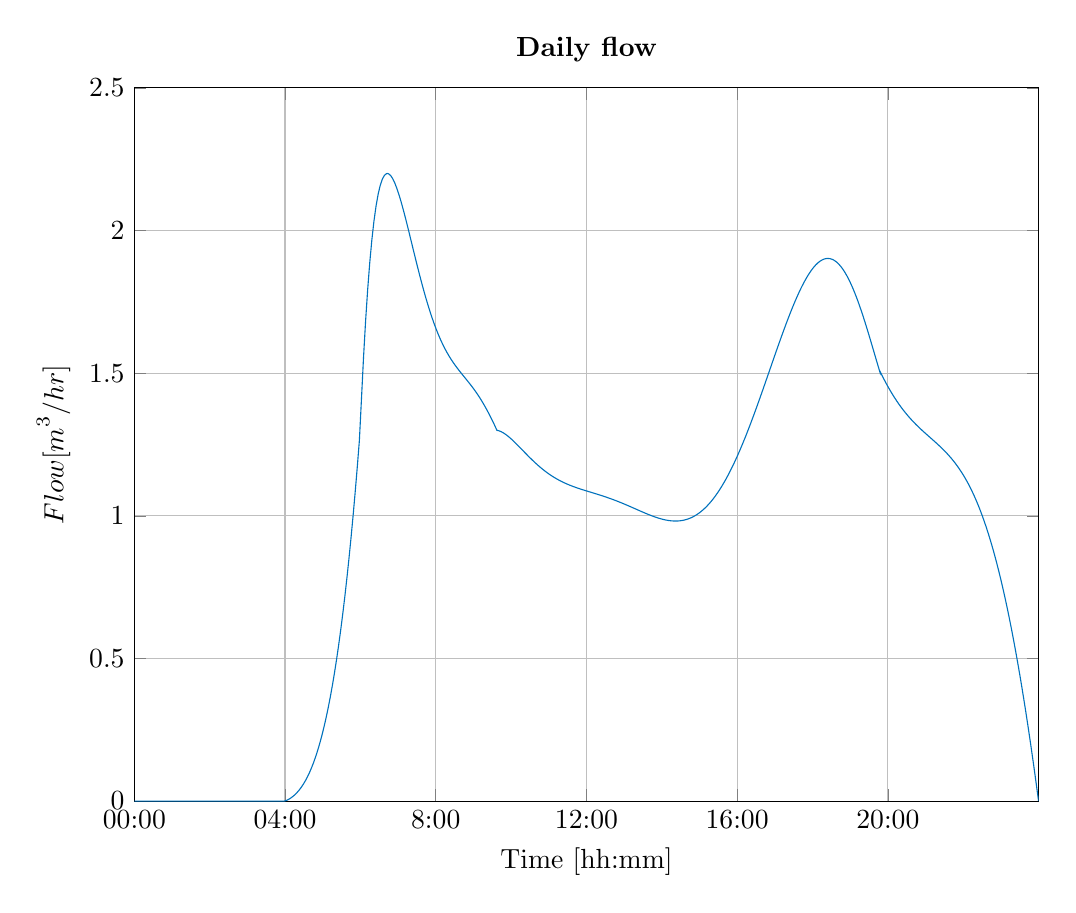
\begin{tikzpicture}

\begin{axis}[%
width=4.521in,
height=3.566in,
at={(0.758in,0.481in)},
scale only axis,
xmin=0,
xmax=24,
xtick={0,4,8,12,16,20,24},
xticklabels={{00:00},{04:00},{8:00},{12:00},{16:00},{20:00}},
xlabel={Time [hh:mm]},
xmajorgrids,
ymin=0,
ymax=2.5,
ylabel={$\text{Flow [m}^\text{3}\text{/hr]}$},
ymajorgrids,
axis background/.style={fill=white},
title style={font=\bfseries},
title={Daily flow}
]
\addplot [color=mycolor1,solid,forget plot]
  table[row sep=crcr]{%
0.000277777777777778	0\\
0.0558333333333333	0\\
0.111111111111111	0\\
0.166388888888889	0\\
0.221666666666667	0\\
0.276944444444444	0\\
0.332222222222222	0\\
0.3875	0\\
0.442777777777778	0\\
0.498055555555556	0\\
0.553333333333333	0\\
0.608611111111111	0\\
0.663888888888889	0\\
0.719166666666667	0\\
0.774722222222222	0\\
0.83	0\\
0.885277777777778	0\\
0.940555555555556	0\\
0.995833333333333	0\\
1.05111111111111	0\\
1.10638888888889	0\\
1.16166666666667	0\\
1.21694444444444	0\\
1.27222222222222	0\\
1.3275	0\\
1.38277777777778	0\\
1.43805555555556	0\\
1.49361111111111	0\\
1.54888888888889	0\\
1.60416666666667	0\\
1.65944444444444	0\\
1.71472222222222	0\\
1.77	0\\
1.82527777777778	0\\
1.88055555555556	0\\
1.93583333333333	0\\
1.99111111111111	0\\
2.04638888888889	0\\
2.10166666666667	0\\
2.15694444444444	0\\
2.2125	0\\
2.26777777777778	0\\
2.32305555555556	0\\
2.37833333333333	0\\
2.43361111111111	0\\
2.48888888888889	0\\
2.54416666666667	0\\
2.59944444444444	0\\
2.65472222222222	0\\
2.71	0\\
2.76527777777778	0\\
2.82055555555556	0\\
2.87583333333333	0\\
2.93138888888889	0\\
2.98666666666667	0\\
3.04194444444444	0\\
3.09722222222222	0\\
3.1525	0\\
3.20777777777778	0\\
3.26305555555556	0\\
3.31833333333333	0\\
3.37361111111111	0\\
3.42888888888889	0\\
3.48416666666667	0\\
3.53944444444444	0\\
3.59472222222222	0\\
3.65027777777778	0\\
3.70555555555556	0\\
3.76083333333333	0\\
3.81611111111111	0\\
3.87138888888889	0\\
3.92666666666667	0\\
3.98194444444444	0\\
4.03722222222222	0.00211951125744408\\
4.0925	0.00585317652957422\\
4.14777777777778	0.0103521562404917\\
4.20305555555556	0.0156924481264725\\
4.25833333333333	0.0219535197955126\\
4.31361111111111	0.0292183140410548\\
4.36916666666667	0.0376181378904421\\
4.42444444444444	0.047159272029085\\
4.47972222222222	0.0579742801903056\\
4.535	0.0701599976198309\\
4.59027777777778	0.0838167021607384\\
4.64555555555556	0.0990480959175509\\
4.70083333333333	0.115961282982026\\
4.75611111111111	0.134666743220625\\
4.81138888888889	0.15527830212367\\
4.86666666666667	0.177913096716188\\
4.92194444444444	0.202691537530468\\
4.97722222222222	0.229737266640256\\
5.0325	0.259177111756696\\
5.08777777777778	0.291141036385921\\
5.14333333333333	0.325942999303699\\
5.19861111111111	0.363371628598894\\
5.25388888888889	0.403733191224315\\
5.30916666666667	0.447169631061583\\
5.36444444444444	0.493825719141305\\
5.41972222222222	0.543848980151002\\
5.475	0.597389615004768\\
5.53027777777778	0.654600419474559\\
5.58555555555556	0.715636698883249\\
5.64083333333333	0.780656178859284\\
5.69611111111111	0.849818912153093\\
5.75138888888889	0.92328718151516\\
5.80666666666667	1.00122539863582\\
5.86222222222222	1.08422693797887\\
5.9175	1.17163084511497\\
5.97277777777778	1.26401049843678\\
6.02805555555556	1.4087687466822\\
6.08333333333333	1.55626229027462\\
6.13861111111111	1.68444700069439\\
6.19388888888889	1.79481723723359\\
6.24916666666667	1.88879654568011\\
6.30444444444444	1.96773924882562\\
6.35972222222222	2.03293203698813\\
6.415	2.08559555852159\\
6.47027777777778	2.12688601033793\\
6.52555555555556	2.15789672841443\\
6.58111111111111	2.17974745400618\\
6.63638888888889	2.19319599381913\\
6.69166666666667	2.19928799785921\\
6.71527777777778	2.19986132051438\\
6.74694444444444	2.19888098364334\\
6.80222222222222	2.19277756833089\\
6.8575	2.18172705923324\\
6.91277777777778	2.16642704433817\\
6.96805555555556	2.14752498282049\\
7.02333333333333	2.12561979555395\\
7.07861111111111	2.1012634556333\\
7.13388888888889	2.07496257888664\\
7.18916666666667	2.04718001439304\\
7.24444444444444	2.01833643499826\\
7.3	1.98866243561785\\
7.35527777777778	1.95879718239166\\
7.41055555555556	1.92889721483563\\
7.46583333333333	1.89923023005929\\
7.52111111111111	1.87002970949847\\
7.57638888888889	1.84149650945383\\
7.63166666666667	1.81380045157769\\
7.68694444444444	1.7870819134194\\
7.74222222222222	1.76145341891732\\
7.7975	1.7370012289254\\
7.85277777777778	1.7137869317273\\
7.90805555555556	1.69184903355736\\
7.96333333333333	1.67120454909763\\
8.01888888888889	1.65175656629258\\
8.07416666666667	1.63367823588564\\
8.12944444444445	1.61683108910686\\
8.18472222222222	1.6011620076358\\
8.24	1.58660434217862\\
8.29527777777778	1.57307950299012\\
8.35055555555556	1.56049855038675\\
8.40583333333333	1.54876378526295\\
8.46111111111111	1.53777033960758\\
8.51638888888889	1.5274077670203\\
8.57166666666667	1.51756163321886\\
8.62694444444444	1.50811510657251\\
8.68222222222222	1.49895054859231\\
8.73777777777778	1.48990610347656\\
8.79305555555556	1.48095726396739\\
8.84833333333333	1.47194799911762\\
8.90361111111111	1.46277338015368\\
8.95888888888889	1.45333563203284\\
9.01416666666667	1.44354572394828\\
9.06944444444444	1.43332495986812\\
9.12472222222222	1.42260656900878\\
9.18	1.41133729639439\\
9.23527777777778	1.39947899334825\\
9.29055555555555	1.38701020801604\\
9.34583333333333	1.37392777586632\\
9.40111111111111	1.3602484102364\\
9.45666666666667	1.34593742681342\\
9.51194444444444	1.33119949371373\\
9.56722222222222	1.31605043591576\\
9.6225	1.29976187213801\\
9.67777777777778	1.29794695465882\\
9.73305555555556	1.29501877905895\\
9.78833333333333	1.2911279331176\\
9.84361111111111	1.28641339000563\\
9.89888888888889	1.28100305956791\\
9.95416666666667	1.27501432476512\\
10.0094444444444	1.26855456337012\\
10.0647222222222	1.26172165523848\\
10.12	1.25460447519825\\
10.1752777777778	1.24728337176778\\
10.2308333333333	1.23979296080759\\
10.2861111111111	1.23227307550874\\
10.3413888888889	1.22474400495921\\
10.3966666666667	1.2172564700505\\
10.4519444444444	1.20985485501197\\
10.5072222222222	1.20257760472525\\
10.5625	1.19545760935293\\
10.6177777777778	1.18852257606597\\
10.6730555555556	1.18179538827351\\
10.7283333333333	1.17529445242049\\
10.7836111111111	1.1690340326478\\
10.8388888888889	1.16302457332389\\
10.8941666666667	1.15727300974708\\
10.9497222222222	1.1517561427058\\
11.005	1.14652994015127\\
11.0602777777778	1.14156430236167\\
11.1155555555556	1.13685499320668\\
11.1708333333333	1.13239565050746\\
11.2261111111111	1.12817802934699\\
11.2813888888889	1.12419223452522\\
11.3366666666667	1.12042694280257\\
11.3919444444444	1.11686961462139\\
11.4472222222222	1.11350669594424\\
11.5025	1.11032381008448\\
11.5577777777778	1.10730593976925\\
11.6130555555556	1.10443759965919\\
11.6686111111111	1.1016895686476\\
11.7238888888889	1.09907331888935\\
11.7791666666667	1.09655884062358\\
11.8344444444444	1.09413031742615\\
11.8897222222222	1.0917721907564\\
11.945	1.08946927873142\\
12.0002777777778	1.0872068865964\\
12.0555555555556	1.08497090908368\\
12.1108333333333	1.08274792464005\\
12.1661111111111	1.08052528204344\\
12.2213888888889	1.07829117932525\\
12.2766666666667	1.07603473510241\\
12.3319444444444	1.07374605287431\\
12.3875	1.07140445337562\\
12.4427777777778	1.06902556046807\\
12.4980555555556	1.06659115535702\\
12.5533333333333	1.06409578956812\\
12.6086111111111	1.06153521765207\\
12.6638888888889	1.05890642141888\\
12.7191666666667	1.05620762814302\\
12.7744444444444	1.05343832291851\\
12.8297222222222	1.05059925526122\\
12.885	1.04769244035276\\
12.9402777777778	1.04472115479229\\
12.9955555555556	1.04168992726159\\
13.0508333333333	1.03860452423975\\
13.1063888888889	1.03545608342688\\
13.1616666666667	1.03228430658388\\
13.2169444444444	1.02908291640403\\
13.2722222222222	1.02586239975415\\
13.3275	1.02263434111511\\
13.3827777777778	1.01941138204336\\
13.4380555555556	1.01620717713635\\
13.4933333333333	1.0130363459243\\
13.5486111111111	1.00991442201346\\
13.6038888888889	1.00685779854771\\
13.6591666666667	1.00388367079712\\
13.7144444444444	1.00100997593932\\
13.7697222222222	0.998255330065261\\
13.8252777777778	0.995626197493037\\
13.8805555555556	0.993168728937686\\
13.9358333333333	0.990889667973437\\
13.9911111111111	0.988809671194725\\
14.0463888888889	0.986949724968917\\
14.1016666666667	0.985331070030453\\
14.1569444444444	0.983975124720065\\
14.2122222222222	0.982903406900816\\
14.2675	0.982137454752601\\
14.3227777777778	0.981698746884653\\
14.3644444444444	0.98159731425296\\
14.3780555555556	0.981608621278948\\
14.4333333333333	0.981888194172414\\
14.4886111111111	0.982558278030602\\
14.5438888888889	0.983639299883856\\
14.5994444444444	0.985159937688267\\
14.6547222222222	0.987124474853235\\
14.71	0.989558190732782\\
14.7652777777778	0.992479148397723\\
14.8205555555556	0.995904618113898\\
14.8758333333333	0.999850997857995\\
14.9311111111111	1.00433373466941\\
14.9863888888889	1.00936724757682\\
15.0416666666667	1.01496485157146\\
15.0969444444444	1.02113868321183\\
15.1522222222222	1.02789962806129\\
15.2075	1.03525725006291\\
15.2627777777778	1.04321972270872\\
15.3183333333333	1.0518384021769\\
15.3736111111111	1.06103231562632\\
15.4288888888889	1.0708466210025\\
15.4841666666667	1.08128328352314\\
15.5394444444444	1.09234257224404\\
15.5947222222222	1.10402300747149\\
15.65	1.11632131159812\\
15.7052777777778	1.12923236374515\\
15.7605555555556	1.14274915779651\\
15.8158333333333	1.15686276408305\\
15.8711111111111	1.17156229574311\\
15.9263888888889	1.1868348787402\\
15.9816666666667	1.20266562622384\\
16.0372222222222	1.21912122481243\\
16.0925	1.23601806377866\\
16.1477777777778	1.25341603514012\\
16.2030555555556	1.27129203037801\\
16.2583333333333	1.28962087307738\\
16.3136111111111	1.30837532327276\\
16.3688888888889	1.32752608786374\\
16.4241666666667	1.34704183639587\\
16.4794444444444	1.36688922309708\\
16.5347222222222	1.38703291485729\\
16.59	1.40743562589638\\
16.6452777777778	1.42805815832532\\
16.7005555555556	1.44885944990105\\
16.7561111111111	1.46990210903324\\
16.8113888888889	1.49093089726747\\
16.8666666666667	1.51200441479996\\
16.9219444444444	1.53307474957772\\
16.9772222222222	1.55409246998622\\
17.0325	1.57500671587293\\
17.0877777777778	1.59576529817844\\
17.1430555555556	1.61631480601724\\
17.1983333333333	1.63660072256095\\
17.2536111111111	1.65656754898519\\
17.3088888888889	1.67615893718046\\
17.3641666666667	1.69531783113834\\
17.4194444444444	1.71398661772477\\
17.475	1.73219686213777\\
17.5302777777778	1.74970797781912\\
17.5855555555556	1.76655415230835\\
17.6408333333333	1.78267723434388\\
17.6961111111111	1.79801940929771\\
17.7513888888889	1.81252340719467\\
17.8066666666667	1.82613272111999\\
17.8619444444444	1.838791835535\\
17.9172222222222	1.85044646581497\\
17.9725	1.86104380787853\\
18.0277777777778	1.87053279919109\\
18.0830555555556	1.8788643904715\\
18.1383333333333	1.88599182905835\\
18.1938888888889	1.8918972737346\\
18.2491666666667	1.89648024070099\\
18.3044444444444	1.8997353982704\\
18.3597222222222	1.9016282618385\\
18.4069444444444	1.9021431401697\\
18.415	1.90212823626733\\
18.4702777777778	1.90120896985175\\
18.5255555555556	1.89884872240134\\
18.5808333333333	1.89503074389887\\
18.6361111111111	1.88974366736024\\
18.6913888888889	1.88298191498533\\
18.7466666666667	1.87474611617671\\
18.8019444444444	1.8650435400998\\
18.8572222222222	1.85388854156105\\
18.9127777777778	1.84123621079203\\
18.9680555555556	1.82724313566847\\
19.0233333333333	1.81188809466255\\
19.0786111111111	1.79521856553378\\
19.1338888888889	1.77729155235771\\
19.1891666666667	1.75817411675875\\
19.2444444444444	1.73794392277829\\
19.2997222222222	1.7166897985046\\
19.355	1.69451231088483\\
19.4102777777778	1.67152435764328\\
19.4655555555556	1.64785177354625\\
19.5208333333333	1.62363395253621\\
19.5761111111111	1.59902448605672\\
19.6313888888889	1.57419181761375\\
19.6869444444444	1.54919515996941\\
19.7422222222222	1.52448553479618\\
19.7944444444444	1.50148617480692\\
19.7975	1.50484943861782\\
19.8527777777778	1.49006060357303\\
19.9080555555556	1.47582023115203\\
19.9633333333333	1.46212706790136\\
20.0186111111111	1.44897720965004\\
20.0738888888889	1.4363641852103\\
20.1291666666667	1.42427904006465\\
20.1844444444444	1.41271042004401\\
20.2397222222222	1.40164465509634\\
20.295	1.39106584292393\\
20.3502777777778	1.38095593269772\\
20.4058333333333	1.37124735720399\\
20.4611111111111	1.36201500795171\\
20.5163888888889	1.35318522882293\\
20.5716666666667	1.34473220302491\\
20.6269444444444	1.33662838410874\\
20.6822222222222	1.32884457975155\\
20.7375	1.32135003545733\\
20.7927777777778	1.31411251817597\\
20.8480555555556	1.30709840010377\\
20.9033333333333	1.30027274231157\\
20.9586111111111	1.29359937846363\\
21.0138888888889	1.28704099855915\\
21.0691666666667	1.2805592325423\\
21.1247222222222	1.27408237622882\\
21.18	1.26763478852089\\
21.2352777777778	1.26114297343352\\
21.2905555555556	1.25456515458041\\
21.3458333333333	1.24785891438636\\
21.4011111111111	1.24098127794658\\
21.4563888888889	1.2338887966957\\
21.5116666666667	1.22653763204957\\
21.5669444444444	1.21888363916487\\
21.6222222222222	1.21088245064892\\
21.6775	1.20248956017425\\
21.7327777777778	1.19366040630174\\
21.7880555555556	1.1843504560589\\
21.8436111111111	1.17446446478745\\
21.8988888888889	1.16405688283689\\
21.9541666666667	1.15303569387437\\
22.0094444444444	1.14135731808511\\
22.0647222222222	1.12897862310946\\
22.12	1.11585700770736\\
22.1752777777778	1.10195048554515\\
22.2305555555556	1.0872177687875\\
22.2858333333333	1.07161835186162\\
22.3411111111111	1.05511259513981\\
22.3963888888889	1.03766180866286\\
22.4516666666667	1.01922833578637\\
22.5069444444444	0.999775636944894\\
22.5625	0.979162600711326\\
22.6177777777778	0.957561163704225\\
22.6730555555556	0.93483826063619\\
22.7283333333333	0.910962664619405\\
22.7836111111111	0.885904684738311\\
22.8388888888889	0.859636249777512\\
22.8941666666667	0.832130991877173\\
22.9494444444444	0.803364330242804\\
23.0047222222222	0.773313554859566\\
23.06	0.741957910165799\\
23.1152777777778	0.709278678799054\\
23.1705555555556	0.675259265251493\\
23.2258333333333	0.639885279620451\\
23.2813888888889	0.602956526260811\\
23.3366666666667	0.564832530375605\\
23.3919444444444	0.525324832876606\\
23.4472222222222	0.48442871604508\\
23.5025	0.442142086792164\\
23.5577777777778	0.398465560078633\\
23.6130555555556	0.353402542923752\\
23.6683333333333	0.30695931774801\\
23.7236111111111	0.259145126454477\\
23.7788888888889	0.209972253812317\\
23.8341666666667	0.159456111379547\\
23.8894444444444	0.107615321031556\\
23.9447222222222	0.0544717987796408\\
24	5.08384535933146e-05\\
};
\end{axis}
\end{tikzpicture}%
\caption{A daily flow profile for zone 2.}
\label{fig:APP_flow_profile_zone2}
\end{figure} 

\begin{figure}[H]
\centering
% This file was created by matlab2tikz.
%
%The latest updates can be retrieved from
%  http://www.mathworks.com/matlabcentral/fileexchange/22022-matlab2tikz-matlab2tikz
%where you can also make suggestions and rate matlab2tikz.
%
\definecolor{mycolor1}{rgb}{0.00000,0.44700,0.74100}%
%
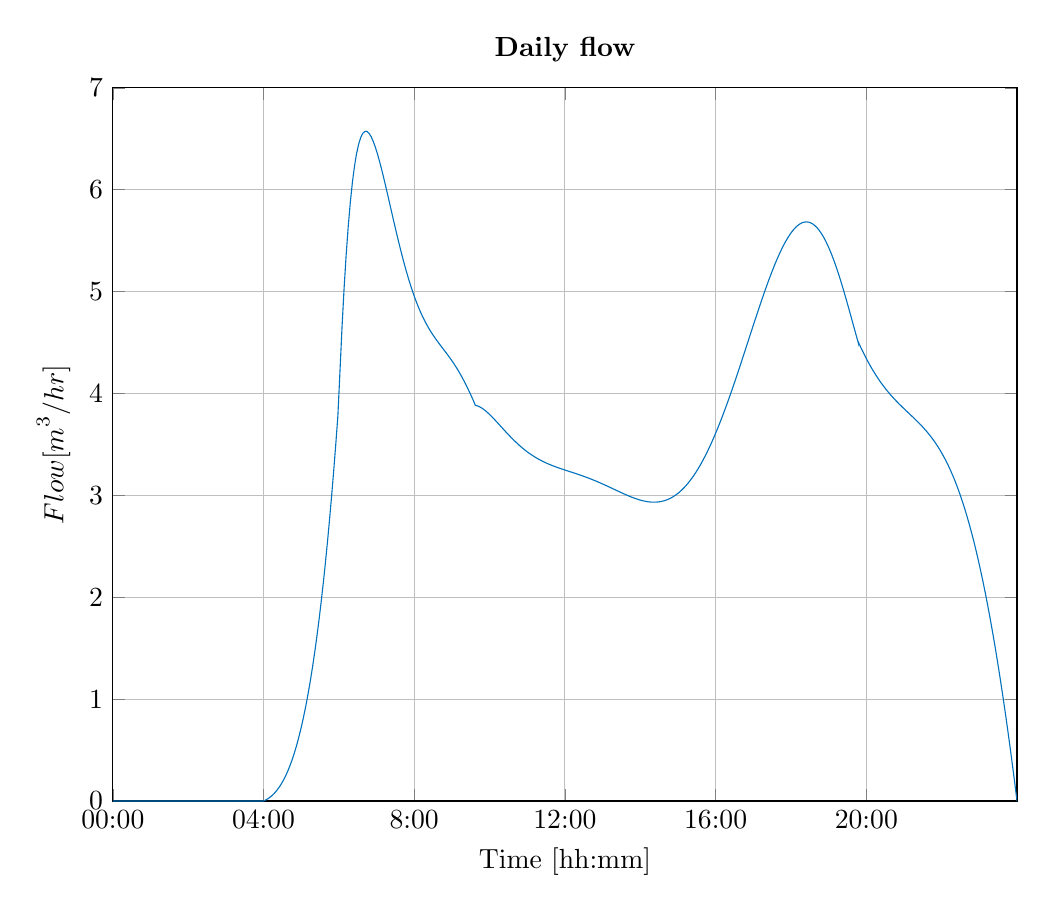
\begin{tikzpicture}

\begin{axis}[%
width=4.521in,
height=3.566in,
at={(0.758in,0.481in)},
scale only axis,
xmin=0,
xmax=24,
xtick={0,4,8,12,16,20,24},
xticklabels={{00:00},{04:00},{8:00},{12:00},{16:00},{20:00}},
xlabel={Time [hh:mm]},
xmajorgrids,
ymin=0,
ymax=7,
ylabel={$\text{Flow [m}^\text{3}\text{/hr]}$},
ymajorgrids,
axis background/.style={fill=white},
title style={font=\bfseries},
title={Daily flow}
]
\addplot [color=mycolor1,solid,forget plot]
  table[row sep=crcr]{%
0.000277777777777778	0\\
0.0558333333333333	0\\
0.111111111111111	0\\
0.166388888888889	0\\
0.221666666666667	0\\
0.276944444444444	0\\
0.332222222222222	0\\
0.3875	0\\
0.442777777777778	0\\
0.498055555555556	0\\
0.553333333333333	0\\
0.608611111111111	0\\
0.663888888888889	0\\
0.719166666666667	0\\
0.774722222222222	0\\
0.83	0\\
0.885277777777778	0\\
0.940555555555556	0\\
0.995833333333333	0\\
1.05111111111111	0\\
1.10638888888889	0\\
1.16166666666667	0\\
1.21694444444444	0\\
1.27222222222222	0\\
1.3275	0\\
1.38277777777778	0\\
1.43805555555556	0\\
1.49361111111111	0\\
1.54888888888889	0\\
1.60416666666667	0\\
1.65944444444444	0\\
1.71472222222222	0\\
1.77	0\\
1.82527777777778	0\\
1.88055555555556	0\\
1.93583333333333	0\\
1.99111111111111	0\\
2.04638888888889	0\\
2.10166666666667	0\\
2.15694444444444	0\\
2.2125	0\\
2.26777777777778	0\\
2.32305555555556	0\\
2.37833333333333	0\\
2.43361111111111	0\\
2.48888888888889	0\\
2.54416666666667	0\\
2.59944444444444	0\\
2.65472222222222	0\\
2.71	0\\
2.76527777777778	0\\
2.82055555555556	0\\
2.87583333333333	0\\
2.93138888888889	0\\
2.98666666666667	0\\
3.04194444444444	0\\
3.09722222222222	0\\
3.1525	0\\
3.20777777777778	0\\
3.26305555555556	0\\
3.31833333333333	0\\
3.37361111111111	0\\
3.42888888888889	0\\
3.48416666666667	0\\
3.53944444444444	0\\
3.59472222222222	0\\
3.65027777777778	0\\
3.70555555555556	0\\
3.76083333333333	0\\
3.81611111111111	0\\
3.87138888888889	0\\
3.92666666666667	0\\
3.98194444444444	0\\
4.03722222222222	0.00633403075201496\\
4.0925	0.017491862808034\\
4.14777777777778	0.0309367906146487\\
4.20305555555556	0.0468959287941403\\
4.25833333333333	0.0656067614698268\\
4.31361111111111	0.0873171581458113\\
4.36916666666667	0.112419521903807\\
4.42444444444444	0.140932622190965\\
4.47972222222222	0.173252617678543\\
4.535	0.209668894621113\\
4.59027777777778	0.250481127266484\\
4.64555555555556	0.295999223059964\\
4.70083333333333	0.346543256079233\\
4.75611111111111	0.402443388699786\\
4.81138888888889	0.464039781490967\\
4.86666666666667	0.531682491342598\\
4.92194444444444	0.605731357822267\\
4.97722222222222	0.686555877763078\\
5.0325	0.774535068082148\\
5.08777777777778	0.870057316829602\\
5.14333333333333	0.974060870751515\\
5.19861111111111	1.08591405772039\\
5.25388888888889	1.20653213793625\\
5.30916666666667	1.33633930207421\\
5.36444444444444	1.47576818957257\\
5.41972222222222	1.62525966900617\\
5.475	1.78526260669055\\
5.53027777777778	1.95623362351646\\
5.58555555555556	2.13863684001526\\
5.64083333333333	2.33294360965462\\
5.69611111111111	2.53963224036502\\
5.75138888888889	2.75918770429675\\
5.80666666666667	2.99210133580762\\
5.86222222222222	3.24014639846865\\
5.9175	3.50134767008346\\
5.97277777777778	3.77741865717813\\
6.02805555555556	4.21001989615431\\
6.08333333333333	4.65079539925999\\
6.13861111111111	5.03386762635261\\
6.19388888888889	5.3637023794784\\
6.24916666666667	5.64455383882438\\
6.30444444444444	5.88046931585461\\
6.35972222222222	6.07529400649055\\
6.415	6.23267574425238\\
6.47027777777778	6.35606975343764\\
6.52555555555556	6.44874340225583\\
6.58111111111111	6.51404296948667\\
6.63638888888889	6.55423311447681\\
6.69166666666667	6.57243869880469\\
6.71527777777778	6.57415203876262\\
6.74694444444444	6.57122236152374\\
6.80222222222222	6.55298267530097\\
6.8575	6.51995889955831\\
6.91277777777778	6.474235733658\\
6.96805555555556	6.41774807004736\\
7.02333333333333	6.35228574740691\\
7.07861111111111	6.27949830382899\\
7.13388888888889	6.2008997299676\\
7.18916666666667	6.11787322220348\\
7.24444444444444	6.03167593580406\\
7.3	5.94299698967878\\
7.35527777777778	5.8537464930433\\
7.41055555555556	5.76439225474001\\
7.46583333333333	5.67573427133324\\
7.52111111111111	5.58847028792319\\
7.57638888888889	5.50320055137358\\
7.63166666666667	5.42043256338536\\
7.68694444444444	5.3405858337447\\
7.74222222222222	5.26399663341188\\
7.7975	5.19092274771347\\
7.85277777777778	5.1215482294972\\
7.90805555555556	5.05598815230725\\
7.96333333333333	4.99429336348829\\
8.01888888888889	4.93617424724431\\
8.07416666666667	4.88214825406287\\
8.12944444444445	4.83180157842916\\
8.18472222222222	4.78497547946651\\
8.24	4.74147077980546\\
8.29527777777778	4.70105261876238\\
8.35055555555556	4.66345520549103\\
8.40583333333333	4.62838657214418\\
8.46111111111111	4.59553332703538\\
8.51638888888889	4.56456540780055\\
8.57166666666667	4.53514083453266\\
8.62694444444444	4.50691046299414\\
8.68222222222222	4.47952273770072\\
8.73777777777778	4.45249396241261\\
8.79305555555556	4.42575089867711\\
8.84833333333333	4.39882725747868\\
8.90361111111111	4.37140946554597\\
8.95888888888889	4.34320532809814\\
9.01416666666667	4.3139487819726\\
9.06944444444444	4.28340464885444\\
9.12472222222222	4.25137338830948\\
9.18	4.21769585107455\\
9.23527777777778	4.18225803214476\\
9.29055555555555	4.14499582395544\\
9.34583333333333	4.10589976949647\\
9.40111111111111	4.06501981556196\\
9.45666666666667	4.02225231018807\\
9.51194444444444	3.97820889161848\\
9.56722222222222	3.93293685184074\\
9.6225	3.8842594676032\\
9.67777777777778	3.87883569687059\\
9.73305555555556	3.87008502181202\\
9.78833333333333	3.85845746486589\\
9.84361111111111	3.84436833891855\\
9.89888888888889	3.82819989477808\\
9.95416666666667	3.81030292429807\\
10.0094444444444	3.79099831943557\\
10.0647222222222	3.77057858819822\\
10.12	3.74930932761559\\
10.1752777777778	3.72743065435806\\
10.2308333333333	3.70504601582383\\
10.2861111111111	3.68257329501744\\
10.3413888888889	3.66007312464689\\
10.3966666666667	3.63769708101798\\
10.4519444444444	3.61557780370628\\
10.5072222222222	3.59383018290726\\
10.5625	3.57255250887551\\
10.6177777777778	3.55182758280985\\
10.6730555555556	3.53172379038961\\
10.7283333333333	3.51229613815835\\
10.7836111111111	3.49358725363533\\
10.8388888888889	3.47562834918181\\
10.8941666666667	3.45844015051584\\
10.9497222222222	3.44195332820173\\
11.005	3.42633513906477\\
11.0602777777778	3.41149563191321\\
11.1155555555556	3.39742214732864\\
11.1708333333333	3.38409567232577\\
11.2261111111111	3.37149156747048\\
11.2813888888889	3.35958026155802\\
11.3366666666667	3.34832791577416\\
11.3919444444444	3.33769705641191\\
11.4472222222222	3.32764717805303\\
11.5025	3.31813531684207\\
11.5577777777778	3.30911659457053\\
11.6130555555556	3.30054473424163\\
11.6686111111111	3.29233241035148\\
11.7238888888889	3.28451390673868\\
11.7791666666667	3.27699954105428\\
11.8344444444444	3.26974204687469\\
11.8897222222222	3.26269492844543\\
11.945	3.25581281563088\\
12.0002777777778	3.24905179404819\\
12.0555555555556	3.24236971096105\\
12.1108333333333	3.23572645687227\\
12.1661111111111	3.22908422437259\\
12.2213888888889	3.22240774399512\\
12.2766666666667	3.21566449738696\\
12.3319444444444	3.20882490945677\\
12.3875	3.20182718147512\\
12.4427777777778	3.19471800440459\\
12.4980555555556	3.18744293248311\\
12.5533333333333	3.17998568327582\\
12.6086111111111	3.17233356951514\\
12.6638888888889	3.16447757152346\\
12.7191666666667	3.15641239161817\\
12.7744444444444	3.14813649103394\\
12.8297222222222	3.13965210965347\\
12.885	3.13096526972474\\
12.9402777777778	3.12208576316538\\
12.9955555555556	3.11302712366615\\
13.0508333333333	3.1038065839997\\
13.1063888888889	3.09439765972078\\
13.1616666666667	3.08491899713218\\
13.2169444444444	3.07535183688372\\
13.2722222222222	3.06572751834043\\
13.3275	3.0560806610203\\
13.3827777777778	3.04644904344749\\
13.4380555555556	3.03687347155777\\
13.4933333333333	3.02739763492984\\
13.5486111111111	3.01806795480322\\
13.6038888888889	3.00893342109344\\
13.6591666666667	3.00004542082146\\
13.7144444444444	2.99145755815391\\
13.7697222222222	2.98322546614878\\
13.8252777777778	2.97536846302832\\
13.8805555555556	2.96802446740337\\
13.9358333333333	2.96121363203623\\
13.9911111111111	2.95499768790562\\
14.0463888888889	2.94943935149671\\
14.1016666666667	2.94460209945517\\
14.1569444444444	2.94054993919233\\
14.2122222222222	2.93734717553597\\
14.2675	2.93505817402945\\
14.3227777777778	2.93374712219287\\
14.3644444444444	2.93344399692937\\
14.3780555555556	2.93347778729027\\
14.4333333333333	2.93431327391409\\
14.4886111111111	2.93631577885446\\
14.5438888888889	2.93954634705176\\
14.5994444444444	2.94409068083719\\
14.6547222222222	2.94996158091978\\
14.71	2.95723459311473\\
14.7652777777778	2.96596369781285\\
14.8205555555556	2.97620050615541\\
14.8758333333333	2.98799402250048\\
14.9311111111111	3.00139040938778\\
14.9863888888889	3.01643275720933\\
15.0416666666667	3.03316085700834\\
15.0969444444444	3.05161097815327\\
15.1522222222222	3.07181565148953\\
15.2075	3.09380345828049\\
15.2627777777778	3.11759882451104\\
15.3183333333333	3.14335522500263\\
15.3736111111111	3.17083067733413\\
15.4288888888889	3.20016013328494\\
15.4841666666667	3.2313494657888\\
15.5394444444444	3.26439947890271\\
15.5947222222222	3.29930575065181\\
15.65	3.33605848610536\\
15.7052777777778	3.37464238182799\\
15.7605555555556	3.41503650046704\\
15.8158333333333	3.45721415624818\\
15.8711111111111	3.50114281444619\\
15.9263888888889	3.54678400178429\\
15.9816666666667	3.59409322981343\\
16.0372222222222	3.64326978744523\\
16.0925	3.69376496516512\\
16.1477777777778	3.74575774663261\\
16.2030555555556	3.79917907344181\\
16.2583333333333	3.85395370740466\\
16.3136111111111	3.91000024353766\\
16.3688888888889	3.96723114118818\\
16.4241666666667	4.02555277119459\\
16.4794444444444	4.08486548174098\\
16.5347222222222	4.14506368197237\\
16.59	4.20603594559785\\
16.6452777777778	4.26766513210514\\
16.7005555555556	4.32982852947309\\
16.7561111111111	4.39271323913402\\
16.8113888888889	4.45555649645829\\
16.8666666666667	4.5185334245756\\
16.9219444444444	4.58150084122359\\
16.9772222222222	4.64431102302239\\
17.0325	4.70681197749309\\
17.0877777777778	4.76884774079915\\
17.1430555555556	4.83025869775096\\
17.1983333333333	4.89088192811566\\
17.2536111111111	4.95055157702511\\
17.3088888888889	5.00909925157398\\
17.3641666666667	5.06635444334406\\
17.4194444444444	5.12214497898095\\
17.475	5.17656518916315\\
17.5302777777778	5.2288960955635\\
17.5855555555556	5.27923986556888\\
17.6408333333333	5.32742271766349\\
17.6961111111111	5.37327187634056\\
17.7513888888889	5.41661619375517\\
17.8066666666667	5.45728680242216\\
17.8619444444444	5.49511779752366\\
17.9172222222222	5.5299469527534\\
17.9725	5.56161646631909\\
18.0277777777778	5.58997374093521\\
18.0830555555556	5.61487219580213\\
18.1383333333333	5.6361721134287\\
18.1938888888889	5.65382017642074\\
18.2491666666667	5.66751609504283\\
18.3044444444444	5.67724393587165\\
18.3597222222222	5.68290064376014\\
18.4069444444444	5.6844393264031\\
18.415	5.68439478699544\\
18.4702777777778	5.68164761510609\\
18.5255555555556	5.67459415885257\\
18.5808333333333	5.66318436182494\\
18.6361111111111	5.64738425448117\\
18.6913888888889	5.62717716790415\\
18.7466666666667	5.60256498302521\\
18.8019444444444	5.57356942330402\\
18.8572222222222	5.54023338720845\\
18.9127777777778	5.50242266462126\\
18.9680555555556	5.46060520890518\\
19.0233333333333	5.41471760081236\\
19.0786111111111	5.36490172474547\\
19.1338888888889	5.31132793392448\\
19.1891666666667	5.25419663794378\\
19.2444444444444	5.19373993107731\\
19.2997222222222	5.1302232706756\\
19.355	5.0639471949564\\
19.4102777777778	4.99524909191661\\
19.4655555555556	4.924505011118\\
19.5208333333333	4.85213152289724\\
19.5761111111111	4.77858762596142\\
19.6313888888889	4.70437670350469\\
19.6869444444444	4.62967570927275\\
19.7422222222222	4.55583249415967\\
19.7944444444444	4.48710030274668\\
19.7975	4.49715121251685\\
19.8527777777778	4.45295567657375\\
19.9080555555556	4.41039918789364\\
19.9633333333333	4.36947800060695\\
20.0186111111111	4.33018044733567\\
20.0738888888889	4.29248718932788\\
20.1291666666667	4.2563714665516\\
20.1844444444444	4.22179934776159\\
20.2397222222222	4.18872998083704\\
20.295	4.15711584272642\\
20.3502777777778	4.12690298962267\\
20.4058333333333	4.09788950100845\\
20.4611111111111	4.07029918561291\\
20.5163888888889	4.043911926598\\
20.5716666666667	4.01865057204555\\
20.6269444444444	3.99443280106484\\
20.6822222222222	3.97117137417083\\
20.7375	3.94877438341872\\
20.7927777777778	3.92714550229467\\
20.8480555555556	3.90618423614826\\
20.9033333333333	3.88578617211029\\
20.9586111111111	3.86584322928149\\
21.0138888888889	3.8462439089889\\
21.0691666666667	3.82687354464953\\
21.1247222222222	3.8075178526607\\
21.18	3.78824962812313\\
21.2352777777778	3.76884923274642\\
21.2905555555556	3.74919182033568\\
21.3458333333333	3.72915062854189\\
21.4011111111111	3.70859722947042\\
21.4563888888889	3.68740177972068\\
21.5116666666667	3.66543327034467\\
21.5669444444444	3.64255977715745\\
21.6222222222222	3.61864871089878\\
21.6775	3.59356706711034\\
21.7327777777778	3.56718167663583\\
21.7880555555556	3.53935945538989\\
21.8436111111111	3.50981577049196\\
21.8988888888889	3.47871334350679\\
21.9541666666667	3.44577718920838\\
22.0094444444444	3.41087707196533\\
22.0647222222222	3.37388409333868\\
22.12	3.33467094210814\\
22.1752777777778	3.29311214466382\\
22.2305555555556	3.24908431481581\\
22.2858333333333	3.20246640411824\\
22.3411111111111	3.15313995194961\\
22.3963888888889	3.10098933571503\\
22.4516666666667	3.04590202081822\\
22.5069444444444	2.98776881098561\\
22.5625	2.92616800328182\\
22.6177777777778	2.86161341985598\\
22.6730555555556	2.79370740317289\\
22.7283333333333	2.7223566335736\\
22.7836111111111	2.647472381559\\
22.8388888888889	2.56897075800563\\
22.8941666666667	2.48677296416473\\
22.9494444444444	2.40080554182387\\
23.0047222222222	2.31100062348206\\
23.06	2.217296182403\\
23.1152777777778	2.11963628288503\\
23.1705555555556	2.01797133026024\\
23.2258333333333	1.91225832117788\\
23.2813888888889	1.80189898310312\\
23.3366666666667	1.68796773528432\\
23.3919444444444	1.5699013791746\\
23.4472222222222	1.44768581615784\\
23.5025	1.32131479116502\\
23.5577777777778	1.19079014196909\\
23.6130555555556	1.05612205024034\\
23.6683333333333	0.917329290611105\\
23.7236111111111	0.774439481947772\\
23.7788888888889	0.627489336537386\\
23.8341666666667	0.476524910885698\\
23.8894444444444	0.321601855337078\\
23.9447222222222	0.162785664561123\\
24	0.000151927632992738\\
};
\end{axis}
\end{tikzpicture}%
\caption{A daily flow profile for zone 3.}
\label{fig:APP_flow_profile_zone3}
\end{figure} 

\begin{figure}[H]
\centering
% This file was created by matlab2tikz.
%
%The latest updates can be retrieved from
%  http://www.mathworks.com/matlabcentral/fileexchange/22022-matlab2tikz-matlab2tikz
%where you can also make suggestions and rate matlab2tikz.
%
\definecolor{mycolor1}{rgb}{0.00000,0.44700,0.74100}%
\definecolor{mycolor2}{rgb}{0.85000,0.32500,0.09800}%
\definecolor{mycolor3}{rgb}{0.92900,0.69400,0.12500}%
\definecolor{mycolor4}{rgb}{0.49400,0.18400,0.55600}%
%
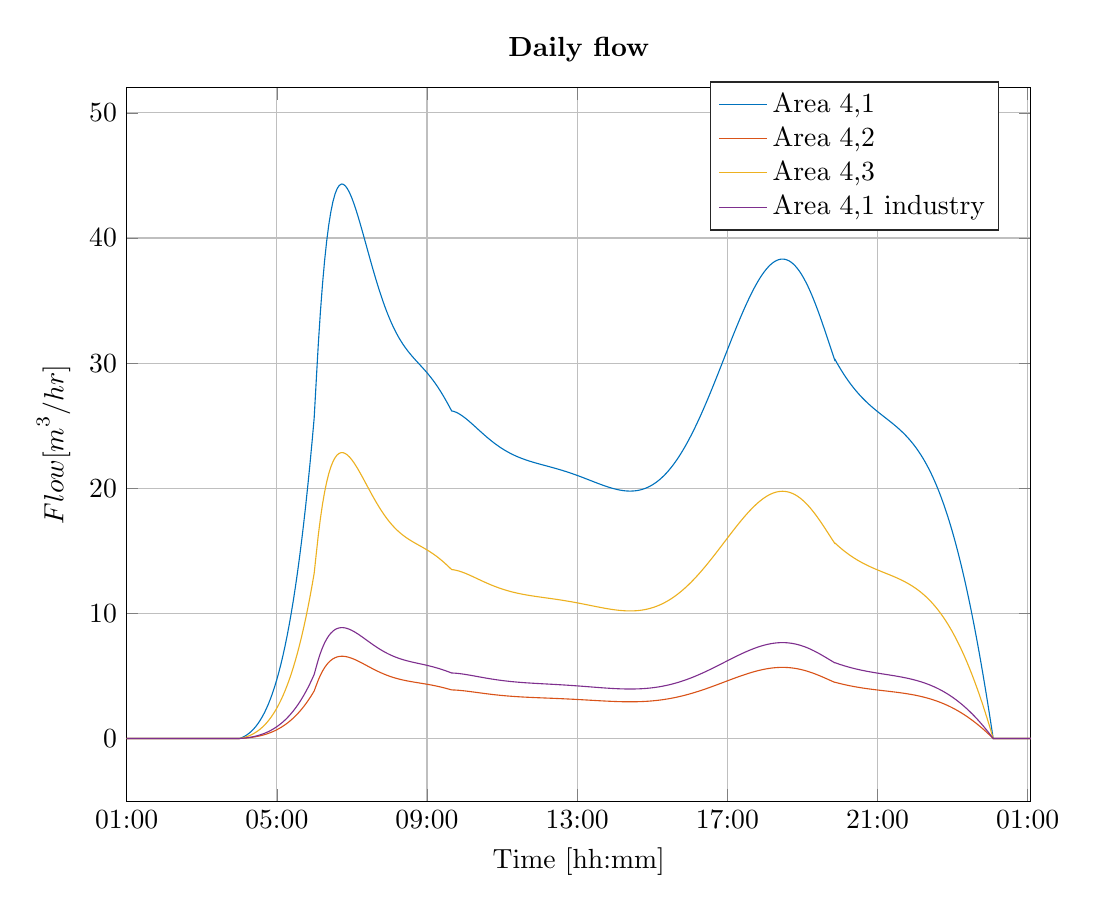
\begin{tikzpicture}

\begin{axis}[%
width=4.521in,
height=3.566in,
at={(0.64in,0.481in)},
scale only axis,
xmin=3600,
xmax=90000,
xtick={3600,17950,32300,46650,61000,75350,89700},
xticklabels={{01:00},{05:00},{09:00},{13:00},{17:00},{21:00},{01:00},{},{},{}},
xlabel={Time [hh:mm]},
xmajorgrids,
ymin=-5,
scaled x ticks = false,
ymax=52,
ylabel={$\text{Flow [m}^\text{3}\text{/hr]}$},
ymajorgrids,
axis background/.style={fill=white},
title style={font=\bfseries},
title={Daily flow},
legend style={at={(0.6450,0.8)},anchor=south west,legend cell align=left,align=left,draw=white!15!black}
]
\addplot [color=mycolor1,solid]
  table[row sep=crcr]{%
3599	0\\
3799	0\\
3998	0\\
4197	0\\
4396	0\\
4595	0\\
4794	0\\
4993	0\\
5192	0\\
5391	0\\
5590	0\\
5789	0\\
5988	0\\
6188	0\\
6387	0\\
6586	0\\
6785	0\\
6984	0\\
7183	0\\
7382	0\\
7581	0\\
7780	0\\
7979	0\\
8178	0\\
8377	0\\
8577	0\\
8776	0\\
8975	0\\
9174	0\\
9373	0\\
9572	0\\
9771	0\\
9970	0\\
10169	0\\
10368	0\\
10567	0\\
10766	0\\
10965	0\\
11165	0\\
11364	0\\
11563	0\\
11762	0\\
11961	0\\
12160	0\\
12359	0\\
12558	0\\
12757	0\\
12956	0\\
13155	0\\
13354	0\\
13554	0\\
13753	0\\
13952	0\\
14151	0\\
14350	0\\
14549	0.0478616674698634\\
14748	0.124184806964865\\
14947	0.216037794955245\\
15146	0.324956831753071\\
15345	0.452548027364151\\
15544	0.600487502551203\\
15743	0.770521410561261\\
15942	0.964465879517816\\
16142	1.18537951395245\\
16341	1.43301713786323\\
16540	1.71044214014931\\
16739	2.01974873106236\\
16938	2.36309961517783\\
17137	2.74272545737682\\
17336	3.16092426949164\\
17535	3.6200607176174\\
17734	4.12256535008644\\
17933	4.67093374610903\\
18132	5.26772558507796\\
18331	5.91556363653736\\
18531	6.62079843271939\\
18730	7.37913488843914\\
18929	8.19676736052568\\
19128	9.07655958137858\\
19327	10.021432126097\\
19526	11.0343609260374\\
19725	12.1183757030377\\
19924	13.2765583243048\\
20123	14.512041077967\\
20322	15.8280048692916\\
20521	17.2276773375662\\
20720	18.7143308936463\\
20920	20.299438710925\\
21119	21.9705196257897\\
21318	23.7386638251055\\
21517	25.6073017704141\\
21716	28.6171641842508\\
21915	31.5579485976407\\
22114	34.1120855607026\\
22313	36.3095695652932\\
22512	38.1789710150114\\
22711	39.7474682654159\\
22910	41.0408796640816\\
23109	42.0836955908396\\
23308	42.8991104979365\\
23508	43.5116365879267\\
23707	43.9359310311559\\
23906	44.1950476559769\\
24105	44.3073118184006\\
24175	44.3151254450439\\
24304	44.2899133085633\\
24503	44.1589383910118\\
24702	43.9294018446922\\
24901	43.6152790032352\\
25100	43.2295377949442\\
25299	42.7841707832406\\
25498	42.2902272064926\\
25697	41.7578450183689\\
25897	41.1934018666942\\
26096	40.6109868662571\\
26295	40.0154359766854\\
26494	39.4135585598243\\
26693	38.8114130545292\\
26892	38.2143390168595\\
27091	37.6269891602271\\
27290	37.0533613954644\\
27489	36.4968308711558\\
27688	35.9601820136712\\
27887	35.4456405673606\\
28086	34.954905634565\\
28285	34.4891817160158\\
28485	34.0470655708191\\
28684	33.6332900539721\\
28883	33.2454904550884\\
29082	32.8832115089587\\
29281	32.5456637105081\\
29480	32.2317553548762\\
29679	31.9401245775647\\
29878	31.6691713945636\\
30077	31.4170897425677\\
30276	31.1818995191019\\
30475	30.9614786227154\\
30674	30.7535949928787\\
30874	30.5549672639391\\
31073	30.3652159210023\\
31272	30.1809544232889\\
31471	29.9998314489239\\
31670	29.8195460789486\\
31869	29.6378798375148\\
32068	29.4527287320785\\
32267	29.2621352934341\\
32466	29.0643206157946\\
32665	28.8577163973044\\
32864	28.6409969798459\\
33063	28.4131113893244\\
33263	28.1720794600276\\
33462	27.9199052373084\\
33661	27.6553812410344\\
33860	27.3788777399722\\
34059	27.0912000485642\\
34258	26.7936205674646\\
34457	26.4879108231627\\
34656	26.1811617588014\\
34855	26.1427996062201\\
35054	26.0822484791968\\
35253	26.0025238650658\\
35452	25.9064081279736\\
35651	25.7964615913248\\
35851	25.6743978444628\\
36050	25.5435943394362\\
36249	25.4054244999429\\
36448	25.2616645027158\\
36647	25.1139195301243\\
36846	24.9636331092286\\
37045	24.8120961741526\\
37244	24.6604558541009\\
37443	24.5097239906285\\
37642	24.3607853869901\\
37841	24.2144057961896\\
38040	24.0712396464498\\
38240	23.931147307733\\
38439	23.795985311666\\
38638	23.6654071495862\\
38837	23.5396937419823\\
39036	23.4190495735519\\
39235	23.3036089339809\\
39434	23.193441922935\\
39633	23.0885602229615\\
39832	22.9889226457783\\
40031	22.8944404519043\\
40230	22.8049824523939\\
40429	22.7203798903499\\
40628	22.6404311108834\\
40828	22.5645372464259\\
41027	22.4932018336635\\
41226	22.4257599824778\\
41425	22.3619209104042\\
41624	22.3013812180461\\
41823	22.2438283480602\\
42022	22.1889438571456\\
42221	22.1364065021338\\
42420	22.0858951426877\\
42619	22.0370914695575\\
42818	21.9896825536906\\
43017	21.9433632279726\\
43217	21.8976110536423\\
43416	21.8525992287088\\
43615	21.8078280568108\\
43814	21.7630440035762\\
44013	21.7180107632865\\
44212	21.6725106859679\\
44411	21.6263460587927\\
44610	21.5793402443015\\
44809	21.5313386809233\\
45008	21.4822097470259\\
45207	21.4318454922843\\
45406	21.380162242667\\
45606	21.326830891331\\
45805	21.2723508662165\\
46004	21.2164506837005\\
46203	21.1591474937498\\
46402	21.1004839378446\\
46601	21.0405280577862\\
46800	20.9793730986594\\
46999	20.9171372128444\\
47198	20.8539630681331\\
47397	20.7900173614133\\
47596	20.7254902443541\\
47795	20.6605946633302\\
47994	20.5955656171447\\
48194	20.5303339396951\\
48393	20.4658297204926\\
48592	20.402022290614\\
48791	20.3392260009996\\
48990	20.2777724257208\\
49189	20.2180092019864\\
49388	20.1602988127313\\
49587	20.1050173135677\\
49786	20.0525530085714\\
49985	20.0033050834381\\
50184	19.957682192268\\
50383	19.9161010055083\\
50583	19.8788102032675\\
50782	19.8466127076352\\
50981	19.8197421666373\\
51180	19.7986321397974\\
51379	19.7837164657406\\
51578	19.7754276541773\\
51712	19.7737956079281\\
51777	19.7741952492232\\
51976	19.7804441953223\\
52175	19.7945931876046\\
52374	19.8170530206011\\
52573	19.8482249365031\\
52772	19.8884989769346\\
52971	19.9382523399749\\
53171	19.9981726695525\\
53370	20.0680088039533\\
53569	20.148364162357\\
53768	20.2395483108162\\
53967	20.3418499811879\\
54166	20.4555355430825\\
54365	20.5808475103174\\
54564	20.7180030780889\\
54763	20.8671927048264\\
54962	21.0285787325697\\
55161	21.202294051025\\
55360	21.3884408170765\\
55560	21.5881191020751\\
55759	21.7993692452879\\
55958	22.0231608068141\\
56157	22.2594611009438\\
56356	22.5082011523584\\
56555	22.7692747788161\\
56754	23.042537755582\\
56953	23.3278070570853\\
57152	23.6248601723791\\
57351	23.933434517864\\
57550	24.2532269276026\\
57749	24.5838932404414\\
57949	24.9267881131493\\
58148	25.2780536977554\\
58347	25.6389096007173\\
58546	26.0088453079527\\
58745	26.3873087511844\\
58944	26.773706520085\\
59143	27.167404195966\\
59342	27.5677268045932\\
59541	27.9739593871231\\
59740	28.3853477094724\\
59939	28.8010990939623\\
60138	29.2203833895323\\
60337	29.6423340750916\\
60537	30.0681816353865\\
60736	30.4927282371871\\
60935	30.9171317704582\\
61134	31.3403940732616\\
61333	31.7614883674884\\
61532	32.1793612673392\\
61731	32.5929349572268\\
61930	33.0011095386013\\
62129	33.4027655364759\\
62328	33.7967665914428\\
62527	34.1819623237595\\
62726	34.5571913778579\\
62926	34.9230841645496\\
63125	35.27480340644\\
63324	35.6130333929472\\
63523	35.9366030923363\\
63722	36.244348581946\\
63921	36.5351172557499\\
64120	36.8077722423273\\
64319	37.0611970241615\\
64518	37.294300269493\\
64717	37.5060208912882\\
64916	37.695333314518\\
65115	37.8612529715556\\
65314	38.002842027885\\
65514	38.1197350288152\\
65713	38.2099334634838\\
65912	38.2733252458911\\
66111	38.309221740352\\
66265	38.3177389797191\\
66310	38.317013227071\\
66509	38.2961760611039\\
66708	38.2462800904735\\
66907	38.1669963150936\\
67106	38.0581048292219\\
67305	37.9195030042633\\
67504	37.7512139479825\\
67703	37.5533952389376\\
67903	37.3251338656978\\
68102	37.0691685352106\\
68301	36.7850479932473\\
68500	36.4735613681301\\
68699	36.135680118532\\
68898	35.7725684553895\\
69097	35.3855940579336\\
69296	34.9763390994471\\
69495	34.5466115489748\\
69694	34.0984568116062\\
69893	33.634169652743\\
70092	33.1563064427748\\
70292	32.6652204075094\\
70491	32.1689538120778\\
70690	31.6684950972024\\
70889	31.1675774997545\\
71088	30.6702619816344\\
71260	30.2467012670642\\
71287	30.2900915921104\\
71486	29.9930657398363\\
71685	29.7070883817591\\
71884	29.4321299115032\\
72083	29.1681074617607\\
72282	28.9148865889408\\
72481	28.6722829596442\\
72680	28.4400640372302\\
72880	28.2168596096975\\
73079	28.0045763677234\\
73278	27.8017059095052\\
73477	27.6078395401385\\
73676	27.4225287998769\\
73875	27.2452871506974\\
74074	27.0755916616804\\
74273	26.912884695302\\
74472	26.756575594639\\
74671	26.6060423673793\\
74870	26.4606333740312\\
75069	26.3196690126641\\
75269	26.181762047693\\
75468	26.0475579603971\\
75667	25.9156049475287\\
75866	25.7851283177211\\
76065	25.6553338569375\\
76264	25.5254095138501\\
76463	25.3945270866804\\
76662	25.2618439081221\\
76861	25.1265045328207\\
77060	24.9876424231173\\
77259	24.8443816341551\\
77458	24.6958385014491\\
77657	24.5411233264487\\
77857	24.3785097342767\\
78056	24.2087233896747\\
78255	24.0300720505576\\
78454	23.8416587495079\\
78653	23.6425889249026\\
78852	23.43197210474\\
79051	23.2089235951239\\
79250	22.9725661640906\\
79449	22.7220317295447\\
79648	22.4564630448209\\
79847	22.1750153836988\\
80046	21.8768582281554\\
80246	21.5595450109666\\
80445	21.2254485257771\\
80644	20.8722492397831\\
80843	20.4991904362003\\
81042	20.1055380433808\\
81241	19.6905823221095\\
81440	19.2536395524448\\
81639	18.7940537189145\\
81838	18.3111981969918\\
82037	17.8044774387479\\
82236	17.2733286595101\\
82435	16.7172235243361\\
82635	16.1326824065839\\
82834	15.5250945318866\\
83033	14.8911868683791\\
83232	14.2305859488115\\
83431	13.5429611949773\\
83630	12.8280266025444\\
83829	12.0855424271655\\
84028	11.3153168716833\\
84227	10.5172077714183\\
84426	9.69112427863591\\
84625	8.83702855303764\\
84824	7.95493744275914\\
85023	7.04492417440511\\
85223	6.10233757334092\\
85422	5.13679549794403\\
85621	4.1439074916505\\
85820	3.12398947087849\\
86019	2.07742216809305\\
86218	1.00465281736833\\
86401	0\\
86417	0\\
86616	0\\
86815	0\\
87014	0\\
87213	0\\
87412	0\\
87612	0\\
87811	0\\
88010	0\\
88209	0\\
88408	0\\
88607	0\\
88806	0\\
89005	0\\
89204	0\\
89403	0\\
89602	0\\
90000	0\\
};
\addlegendentry{Area 4,1};

\addplot [color=mycolor2,solid]
  table[row sep=crcr]{%
3599	0\\
3799	0\\
3998	0\\
4197	0\\
4396	0\\
4595	0\\
4794	0\\
4993	0\\
5192	0\\
5391	0\\
5590	0\\
5789	0\\
5988	0\\
6188	0\\
6387	0\\
6586	0\\
6785	0\\
6984	0\\
7183	0\\
7382	0\\
7581	0\\
7780	0\\
7979	0\\
8178	0\\
8377	0\\
8577	0\\
8776	0\\
8975	0\\
9174	0\\
9373	0\\
9572	0\\
9771	0\\
9970	0\\
10169	0\\
10368	0\\
10567	0\\
10766	0\\
10965	0\\
11165	0\\
11364	0\\
11563	0\\
11762	0\\
11961	0\\
12160	0\\
12359	0\\
12558	0\\
12757	0\\
12956	0\\
13155	0\\
13354	0\\
13554	0\\
13753	0\\
13952	0\\
14151	0\\
14350	0\\
14549	0.00710028180255936\\
14748	0.0184228250217605\\
14947	0.0320492223793003\\
15146	0.0482073693016751\\
15345	0.0671355323234623\\
15544	0.0890823640800493\\
15743	0.114306906530896\\
15942	0.143078582413403\\
16142	0.175851135929245\\
16341	0.212588195200944\\
16540	0.253744214191448\\
16739	0.299629869141819\\
16938	0.350565997430973\\
17137	0.406883518354036\\
17336	0.468923342131185\\
17535	0.537036267147258\\
17734	0.611582865421718\\
17933	0.692933356309431\\
18132	0.781467468431938\\
18331	0.877574289839258\\
18531	0.982195922443594\\
18730	1.09469519004965\\
18929	1.21599102593738\\
19128	1.3465082650137\\
19327	1.48668017480407\\
19526	1.63694823493869\\
19725	1.79776190486959\\
19924	1.96957837981796\\
20123	2.15286233495235\\
20322	2.34808565779734\\
20521	2.55572716887281\\
20720	2.77627233056388\\
20920	3.0114231889665\\
21119	3.25932816256334\\
21318	3.52163248137147\\
21517	3.79884505460662\\
21716	4.24535835961483\\
21915	4.68162393830136\\
22114	5.0605303399952\\
22313	5.38652724971494\\
22512	5.66385308888405\\
22711	5.89653976849929\\
22910	6.08841744227553\\
23109	6.24311925981753\\
23308	6.36408611977997\\
23508	6.45495440917018\\
23707	6.51789852026043\\
23906	6.55633849014062\\
24105	6.57299288668956\\
24175	6.57415203876262\\
24304	6.57041181650709\\
24503	6.55098167809271\\
24702	6.51692991498017\\
24901	6.4703297689161\\
25100	6.41310503299458\\
25299	6.3470348048595\\
25498	6.2737582398154\\
25697	6.19477930401627\\
25897	6.11104412197444\\
26096	6.02464281487946\\
26295	5.93629279768905\\
26494	5.84700423972142\\
26693	5.75767591081538\\
26892	5.66909993449537\\
27091	5.58196654112981\\
27290	5.4968688210775\\
27489	5.41430747787304\\
27688	5.33469558136816\\
27887	5.25836332089683\\
28086	5.18556275841323\\
28285	5.11647258168728\\
28485	5.0508846198317\\
28684	4.98950099222484\\
28883	4.93197089391124\\
29082	4.87822678626446\\
29281	4.82815154614999\\
29480	4.78158321907345\\
29679	4.73831977233886\\
29878	4.69812384820355\\
30077	4.66072751704663\\
30276	4.62583703052387\\
30475	4.59313757473281\\
30674	4.5622980233338\\
30874	4.53283158549684\\
31073	4.50468196016016\\
31272	4.4773467537562\\
31471	4.45047714751611\\
31670	4.42373179994733\\
31869	4.39678159999861\\
32068	4.36931442022513\\
32267	4.34103986992983\\
32466	4.31169404831157\\
32665	4.28104429767759\\
32864	4.24889395655103\\
33063	4.21508711284956\\
33263	4.17933000884771\\
33462	4.14191994481735\\
33661	4.1026777909942\\
33860	4.06165847677637\\
34059	4.01898147061914\\
34258	3.97483553325084\\
34457	3.92948347075326\\
34656	3.88397722505031\\
34855	3.87828619696292\\
35054	3.86930343292533\\
35253	3.85747628069986\\
35452	3.84321750420727\\
35651	3.8269069276083\\
35851	3.80879876200495\\
36050	3.78939405265094\\
36249	3.76889654705036\\
36448	3.74756974114895\\
36647	3.72565176386635\\
36846	3.70335676254554\\
37045	3.68087624735635\\
37244	3.65838039499861\\
37443	3.63601931223958\\
37642	3.61392425970557\\
37841	3.59220883690962\\
38040	3.57097012832554\\
38240	3.55018741982724\\
38439	3.53013612801473\\
38638	3.51076484830304\\
38837	3.49211525526681\\
39036	3.47421768422563\\
39235	3.45709205706402\\
39434	3.44074877307242\\
39633	3.42518956535756\\
39832	3.41040832363483\\
40031	3.39639188339584\\
40230	3.38312078275112\\
40429	3.37056998660284\\
40628	3.35870957943378\\
40828	3.34745071919719\\
41027	3.33686810559657\\
41226	3.32686310213515\\
41425	3.31739257121347\\
41624	3.30841150350928\\
41823	3.29987353111825\\
42022	3.29173141295388\\
42221	3.28393749256906\\
42420	3.27644412877175\\
42619	3.26920410036191\\
42818	3.26217098429212\\
43017	3.25529950899909\\
43217	3.24851217065511\\
43416	3.24183466319726\\
43615	3.23519285663449\\
43814	3.22854913912451\\
44013	3.22186845469703\\
44212	3.21511851496282\\
44411	3.20826998920971\\
44610	3.20129667325793\\
44809	3.19417563788733\\
45008	3.18688735701933\\
45207	3.17941581621549\\
45406	3.17174860242722\\
45606	3.16383689263074\\
45805	3.15575477699682\\
46004	3.14746198091052\\
46203	3.13896104857063\\
46402	3.13025830584381\\
46601	3.12136384673614\\
46800	3.11229150416268\\
46999	3.10305880603746\\
47198	3.09368691713768\\
47397	3.08420056695858\\
47596	3.07462796451394\\
47795	3.06500070041369\\
47994	3.05535363674715\\
48194	3.04567651271804\\
48393	3.03610730717207\\
48592	3.02664147037229\\
48791	3.01732563630324\\
48990	3.0082089940022\\
49189	2.99934311547402\\
49388	2.99078177508811\\
49587	2.98258076072152\\
49786	2.97479767731173\\
49985	2.96749174408537\\
50184	2.96072358490748\\
50383	2.95455501286881\\
50583	2.94902291968129\\
50782	2.94424641889452\\
50981	2.94026017220989\\
51180	2.93712849821384\\
51379	2.93491575689753\\
51578	2.9336861111075\\
51712	2.93344399692937\\
51777	2.93350328374416\\
51976	2.93443031534624\\
52175	2.9365293193663\\
52374	2.93986123720252\\
52573	2.94448559316272\\
52772	2.95046024994984\\
52971	2.95784116492597\\
53171	2.96673035011726\\
53370	2.97709054566539\\
53569	2.98901126884894\\
53768	3.00253844381405\\
53967	3.01771490395241\\
54166	3.03458016521482\\
54365	3.0531702045435\\
54564	3.07351724286139\\
54763	3.09564953469017\\
54962	3.11959116348308\\
55161	3.14536184343757\\
55360	3.17297672953474\\
55560	3.2025990174384\\
55759	3.23393799133826\\
55958	3.26713748554458\\
56157	3.30219265112997\\
56356	3.33909325560095\\
56555	3.37782354681432\\
56754	3.41836212902034\\
56953	3.46068185036243\\
57152	3.50474970132568\\
57351	3.55052672761426\\
57550	3.59796795453961\\
57749	3.64702232576993\\
57949	3.69789080473406\\
58148	3.75000107940876\\
58347	3.80353407849953\\
58546	3.85841406720561\\
58745	3.91455914615849\\
58944	3.97188128289352\\
59143	4.03028636135278\\
59342	4.08967424906017\\
59541	4.14993888181998\\
59740	4.21096836895186\\
59939	4.27264511666528\\
60138	4.33484597199087\\
60337	4.39744238646266\\
60537	4.460616902581\\
60736	4.52359842141341\\
60935	4.58655871601919\\
61134	4.64934970900322\\
61333	4.7118190777594\\
61532	4.77381055242879\\
61731	4.83516423899175\\
61930	4.89571696741947\\
62129	4.95530266351737\\
62328	5.01375274828578\\
62527	5.07089656280736\\
62726	5.12656181990029\\
62926	5.1808420410537\\
63125	5.23301961581908\\
63324	5.28319605858069\\
63523	5.33119764669666\\
63722	5.37685171215669\\
63921	5.41998726577409\\
64120	5.46043565259203\\
64319	5.49803123715681\\
64518	5.53261212032364\\
64717	5.56402088975496\\
64916	5.5921054013216\\
65115	5.61671959434555\\
65314	5.63772434100905\\
65514	5.65506542608248\\
65713	5.66844637033604\\
65912	5.67785054580365\\
66111	5.68317579333198\\
66265	5.6844393264031\\
66310	5.68433166094568\\
66509	5.68124046587969\\
66708	5.67383839505733\\
66907	5.66207664129223\\
67106	5.64592258155172\\
67305	5.62536099087637\\
67504	5.60039529730472\\
67703	5.57104887762718\\
67903	5.5371862865325\\
68102	5.49921381139279\\
68301	5.45706450861086\\
68500	5.41085544542991\\
68699	5.36073073781378\\
68898	5.30686309653841\\
69097	5.24945541691582\\
69296	5.18874241446603\\
69495	5.12499230152653\\
69694	5.05850851408906\\
69893	4.9896314807656\\
70092	4.91874043928682\\
70292	4.84588779072665\\
70491	4.77226660569418\\
70690	4.6980235194415\\
70889	4.62371235792628\\
71088	4.54993556513772\\
71260	4.48710030274668\\
71287	4.49353726057994\\
71486	4.44947345408763\\
71685	4.407048692502\\
71884	4.36625858371511\\
72083	4.32709083435589\\
72282	4.289525499708\\
72481	4.25353523389844\\
72680	4.21908554009987\\
72880	4.18597314726358\\
73079	4.15448091308838\\
73278	4.12438506605859\\
73477	4.09562497625584\\
73676	4.06813411464458\\
73875	4.04184030327419\\
74074	4.01666596530525\\
74273	3.99252837517106\\
74472	3.96933990887471\\
74671	3.94700829381207\\
74870	3.92543685921783\\
75069	3.9045247860968\\
75269	3.88406627795044\\
75468	3.86415709197283\\
75667	3.84458185304801\\
75866	3.82522563565619\\
76065	3.80597061808801\\
76264	3.78669633247073\\
76463	3.76727991501112\\
76662	3.74759635595384\\
76861	3.72751874991917\\
77060	3.70691854598326\\
77259	3.68566579766375\\
77458	3.66362941327093\\
77657	3.64067740596097\\
77857	3.61655366789701\\
78056	3.5913658514955\\
78255	3.56486291252174\\
78454	3.53691178579501\\
78653	3.50737976303432\\
78852	3.4761347426544\\
79051	3.44304548025224\\
79250	3.40798183840312\\
79449	3.37081503706588\\
79648	3.33141790363627\\
79847	3.28966512291887\\
80046	3.24543348750541\\
80246	3.19836004897266\\
80445	3.14879681142805\\
80644	3.09639967201374\\
80843	3.04105637174048\\
81042	2.98265801102665\\
81241	2.92109930000879\\
81440	2.85627880878449\\
81639	2.78809921741142\\
81838	2.71646756609606\\
82037	2.64129550526046\\
82236	2.56249954575803\\
82435	2.4800013090622\\
82635	2.39328459231101\\
82834	2.30314888751374\\
83033	2.20910864015839\\
83232	2.11110844635167\\
83431	2.0090992647929\\
83630	1.90303866671892\\
83829	1.79289108603862\\
84028	1.67862806962992\\
84227	1.56022852735244\\
84426	1.43767898193824\\
84625	1.31097381977632\\
84824	1.1801155402888\\
85023	1.04511500664776\\
85223	0.905282216762484\\
85422	0.762043980613217\\
85621	0.614748973653748\\
85820	0.463444062107368\\
86019	0.308185727662584\\
86218	0.149040317526378\\
86401	0\\
86417	0\\
86616	0\\
86815	0\\
87014	0\\
87213	0\\
87412	0\\
87612	0\\
87811	0\\
88010	0\\
88209	0\\
88408	0\\
88607	0\\
88806	0\\
89005	0\\
89204	0\\
89403	0\\
89602	0\\
90000	0\\
};
\addlegendentry{Area 4,2};

\addplot [color=mycolor3,solid]
  table[row sep=crcr]{%
3599	0\\
3799	0\\
3998	0\\
4197	0\\
4396	0\\
4595	0\\
4794	0\\
4993	0\\
5192	0\\
5391	0\\
5590	0\\
5789	0\\
5988	0\\
6188	0\\
6387	0\\
6586	0\\
6785	0\\
6984	0\\
7183	0\\
7382	0\\
7581	0\\
7780	0\\
7979	0\\
8178	0\\
8377	0\\
8577	0\\
8776	0\\
8975	0\\
9174	0\\
9373	0\\
9572	0\\
9771	0\\
9970	0\\
10169	0\\
10368	0\\
10567	0\\
10766	0\\
10965	0\\
11165	0\\
11364	0\\
11563	0\\
11762	0\\
11961	0\\
12160	0\\
12359	0\\
12558	0\\
12757	0\\
12956	0\\
13155	0\\
13354	0\\
13554	0\\
13753	0\\
13952	0\\
14151	0\\
14350	0\\
14549	0.0246793160526096\\
14748	0.064034461439272\\
14947	0.111397393840624\\
15146	0.167560237205242\\
15345	0.233351163607856\\
15544	0.309634445361409\\
15743	0.397310466220541\\
15942	0.497315691676762\\
16142	0.611227255831437\\
16341	0.738918736510825\\
16540	0.881969734820176\\
16739	1.04146010608868\\
16938	1.21850502395253\\
17137	1.41425470499459\\
17336	1.62989409247532\\
17535	1.86664249915594\\
17734	2.12575320921243\\
17933	2.40851303924187\\
18132	2.71624185836014\\
18331	3.050292067391\\
18531	3.41393824493451\\
18730	3.80496567992113\\
18929	4.22656842090808\\
19128	4.68022311843252\\
19327	5.16743573331317\\
19526	5.68974077018343\\
19725	6.24870047011731\\
19924	6.84590396234597\\
20123	7.48296637506648\\
20322	8.16152790534202\\
20521	8.88325284809369\\
20720	9.64982858418433\\
20920	10.4671711229648\\
21119	11.3288446965693\\
21318	12.2405678317689\\
21517	13.2041094064373\\
21716	14.7561101977328\\
21915	16.272491715914\\
22114	17.5895029419175\\
22313	18.7226101890479\\
22512	19.6865454559471\\
22711	20.4953229477625\\
22910	21.1622555972323\\
23109	21.6999715858648\\
23308	22.1204308650766\\
23508	22.4362728690113\\
23707	22.6550553982746\\
23906	22.7886658931967\\
24105	22.8465536119558\\
24175	22.8505826182909\\
24304	22.8375822713022\\
24503	22.7700465677613\\
24702	22.6516886986835\\
24901	22.4897148834472\\
25100	22.2908118845092\\
25299	22.0611635286896\\
25498	21.8064672281398\\
25697	21.5319505015807\\
25897	21.2409019094547\\
26096	20.9405863410801\\
26295	20.6334974031861\\
26494	20.3231462645636\\
26693	20.0126568892364\\
26892	19.7047825576174\\
27091	19.4019223876408\\
27290	19.1061378558535\\
27489	18.8191693186419\\
27688	18.5424525333048\\
27887	18.2771351792101\\
28086	18.0240933788561\\
28285	17.7839482191336\\
28485	17.5559761350823\\
28684	17.3426175687196\\
28883	17.1426531844458\\
29082	16.955848230014\\
29281	16.7817956062505\\
29480	16.6199323881528\\
29679	16.4695563460211\\
29878	16.3298424665798\\
30077	16.1998594741447\\
30276	16.0785863517435\\
30475	15.9649288622725\\
30674	15.8577360694987\\
30874	15.7553159751215\\
31073	15.6574728866689\\
31272	15.5624605735008\\
31471	15.4690666036488\\
31670	15.3761045348266\\
31869	15.2824304355851\\
32068	15.1869594064692\\
32267	15.0886821010907\\
32466	14.9866812472261\\
32665	14.8801481681366\\
32864	14.7683993035246\\
33063	14.6508927307363\\
33263	14.5266074001921\\
33462	14.3965766747326\\
33661	14.2601779311733\\
33860	14.1176020943271\\
34059	13.9692644152855\\
34258	13.81582099275\\
34457	13.6581852938948\\
34656	13.5000136816546\\
34855	13.4802326807396\\
35054	13.4490101914252\\
35253	13.4079011149277\\
35452	13.3583401451847\\
35651	13.301647483389\\
35851	13.2387067220946\\
36050	13.1712594054424\\
36249	13.1000137235\\
36448	13.0258855412856\\
36647	12.949702552549\\
36846	12.8722090953469\\
37045	12.7940708249504\\
37244	12.7158792452853\\
37443	12.6381561007631\\
37642	12.5613576299631\\
37841	12.4858786845775\\
38040	12.4120567129613\\
38240	12.3398197164982\\
38439	12.2701249942794\\
38638	12.2027938731152\\
38837	12.1379712064109\\
39036	12.0757624343394\\
39235	12.016236801826\\
39434	11.9594304549538\\
39633	11.9053494176935\\
39832	11.853972451783\\
40031	11.8052537997337\\
40230	11.7591258154812\\
40429	11.7155014814803\\
40628	11.6742768167167\\
40828	11.6351430220452\\
41027	11.5983597403424\\
41226	11.563584128698\\
41425	11.5306662484925\\
41624	11.4994496553311\\
41823	11.4697731826296\\
42022	11.4414726287778\\
42221	11.414382348446\\
42420	11.3883367493285\\
42619	11.3631716989368\\
42818	11.3387258390192\\
43017	11.3148418136777\\
43217	11.2912502333989\\
43416	11.2680404057359\\
43615	11.2449546680313\\
43814	11.2218622882142\\
44013	11.1986414179701\\
44212	11.1751798286038\\
44411	11.1513755717792\\
44610	11.1271375664304\\
44809	11.1023861146683\\
45008	11.0770533473186\\
45207	11.051083601043\\
45406	11.0244337302934\\
45606	10.9969340349274\\
45805	10.968842039194\\
46004	10.9400177556987\\
46203	10.9104700276236\\
46402	10.8802208425558\\
46601	10.8493052854639\\
46800	10.8177714370993\\
46999	10.785680221372\\
47198	10.7531052032812\\
47397	10.720132338152\\
47596	10.6868596754962\\
47795	10.6533970186526\\
47994	10.6198655420399\\
48194	10.5862295809561\\
48393	10.5529687253157\\
48592	10.5200671610426\\
48791	10.4876869795685\\
48990	10.455999153234\\
49189	10.4251829371505\\
49388	10.3954252414571\\
49587	10.366919974887\\
49786	10.339867361952\\
49985	10.3144732381459\\
50184	10.2909483212355\\
50383	10.2695074625247\\
50583	10.2502788910392\\
50782	10.2336766242814\\
50981	10.219821140157\\
51180	10.2089359986272\\
51379	10.2012449035684\\
51578	10.1969708736174\\
51712	10.1961293278183\\
51777	10.1963353982365\\
51976	10.1995575951203\\
52175	10.2068533595769\\
52374	10.2184345130618\\
52573	10.2345079514766\\
52772	10.2552747952802\\
52971	10.2809295423056\\
53171	10.3118267682025\\
53370	10.347836964334\\
53569	10.3892712768309\\
53768	10.4362893298527\\
53967	10.489040004647\\
54166	10.5476606516267\\
54365	10.6122763202412\\
54564	10.6829990046846\\
54763	10.7599269126465\\
54962	10.8431437539247\\
55161	10.9327180515615\\
55360	11.0287024815743\\
55560	11.1316642830499\\
55759	11.2405929795645\\
55958	11.3559885135853\\
56157	11.4778340311036\\
56356	11.6060939657929\\
56555	11.7407135660064\\
56754	11.8816184639256\\
56953	12.0287142845286\\
57152	12.1818862926156\\
57351	12.3409990899861\\
57550	12.5058963526261\\
57749	12.6764006178115\\
57949	12.8532103986598\\
58148	13.0343364404208\\
58347	13.2204076190786\\
58546	13.4111606939429\\
58745	13.6063109973826\\
58944	13.805552544216\\
59143	14.0085582037736\\
59342	14.2149799333871\\
59541	14.4244490727863\\
59740	14.6365767098772\\
59939	14.8509541095697\\
60138	15.0671532140572\\
60337	15.2847272117474\\
60537	15.5043105878879\\
60736	15.7232231398064\\
60935	15.9420619200899\\
61134	16.1603122380634\\
61333	16.3774446474538\\
61532	16.5929159820397\\
61731	16.8061704786618\\
61930	17.0166409873362\\
62129	17.2237502637151\\
62328	17.4269123571945\\
62527	17.6255340877463\\
62726	17.819016615785\\
62926	18.0076850053646\\
63125	18.1890449702648\\
63324	18.3634493564207\\
63523	18.5302943348431\\
63722	18.6889797422545\\
63921	18.8389112506693\\
64120	18.9795026454698\\
64319	19.1101782072936\\
64518	19.2303752035234\\
64717	19.3395464968852\\
64916	19.4371632614602\\
65115	19.5227178163229\\
65314	19.5957265779367\\
65514	19.6560011038109\\
65713	19.7025108849011\\
65912	19.7351981253562\\
66111	19.7537077381384\\
66265	19.7580995542483\\
66310	19.7577253282773\\
66509	19.7469808843052\\
66708	19.721252603323\\
66907	19.6803708402362\\
67106	19.6242222031885\\
67305	19.55275377293\\
67504	19.4659774647129\\
67703	19.3639745321007\\
67903	19.2462741912938\\
68102	19.1142886248991\\
68301	18.9677851488853\\
68500	18.8071706681577\\
68699	18.6329461041612\\
68898	18.4457117688192\\
69097	18.246172890131\\
69296	18.0351452974767\\
69495	17.8135612492131\\
69694	17.5824754348512\\
69893	17.3430711236669\\
70092	17.0966664785269\\
70292	16.8434436362394\\
70491	16.5875494979351\\
70690	16.3294937416564\\
70889	16.0712013678791\\
71088	15.814766364705\\
71260	15.5963621741505\\
71287	15.6187358941241\\
71486	15.4655779438984\\
71685	15.3181170221008\\
71884	15.1763378625455\\
72083	15.0401977356626\\
72282	14.9096273171669\\
72481	14.7845315576702\\
72680	14.6647905523394\\
72880	14.5496977671812\\
73079	14.4402363652221\\
73278	14.3356285564938\\
73477	14.2356636021891\\
73676	14.1401102592192\\
73875	14.0487176498718\\
74074	13.9612161308579\\
74273	13.8773181628286\\
74472	13.7967191803633\\
74671	13.7190984603101\\
74870	13.644119992291\\
75069	13.5714333474196\\
75269	13.5003232136885\\
75468	13.4311224260642\\
75667	13.3630823789696\\
75866	13.2958036117489\\
76065	13.2288765971067\\
76264	13.1618826101546\\
76463	13.0943945982108\\
76662	13.0259780496113\\
76861	12.956191863839\\
77060	12.8845892207581\\
77259	12.8107184495198\\
77458	12.7341238987386\\
77657	12.6543468056322\\
77857	12.5704969849341\\
78056	12.4829486172871\\
78255	12.3908291176046\\
78454	12.2936759749973\\
78653	12.1910279190961\\
78852	12.0824257882978\\
79051	11.9674134004125\\
79250	11.8455384209099\\
79449	11.7163532332832\\
79648	11.5794158081903\\
79847	11.4342905723118\\
80046	11.2805492786213\\
80246	11.1169303829862\\
80445	10.9446573890449\\
80644	10.7625342564965\\
80843	10.5701707930709\\
81042	10.3671884832009\\
81241	10.1532213580576\\
81440	9.92791686534956\\
81639	9.69093673827528\\
81838	9.44195786513464\\
82037	9.18067315851651\\
82236	8.9067924250042\\
82435	8.6200432347868\\
82635	8.31863135857426\\
82834	8.00533568832146\\
83033	7.67846852294898\\
83232	7.33783728838288\\
83431	6.98327152578885\\
83630	6.61462376033636\\
83829	6.23177037062165\\
84028	5.83461245865564\\
84227	5.42307671886333\\
84426	4.99711630665961\\
84625	4.55671171013161\\
84824	4.10187161682587\\
85023	3.6326337851954\\
85223	3.14659989075857\\
85422	2.64872927110629\\
85621	2.13675803801893\\
85820	1.61084909014882\\
86019	1.07119874779432\\
86218	0.518037622040429\\
86401	0\\
86417	0\\
86616	0\\
86815	0\\
87014	0\\
87213	0\\
87412	0\\
87612	0\\
87811	0\\
88010	0\\
88209	0\\
88408	0\\
88607	0\\
88806	0\\
89005	0\\
89204	0\\
89403	0\\
89602	0\\
90000	0\\
};
\addlegendentry{Area 4,3};

\addplot [color=mycolor4,solid]
  table[row sep=crcr]{%
3599	0\\
3799	0\\
3998	0\\
4197	0\\
4396	0\\
4595	0\\
4794	0\\
4993	0\\
5192	0\\
5391	0\\
5590	0\\
5789	0\\
5988	0\\
6188	0\\
6387	0\\
6586	0\\
6785	0\\
6984	0\\
7183	0\\
7382	0\\
7581	0\\
7780	0\\
7979	0\\
8178	0\\
8377	0\\
8577	0\\
8776	0\\
8975	0\\
9174	0\\
9373	0\\
9572	0\\
9771	0\\
9970	0\\
10169	0\\
10368	0\\
10567	0\\
10766	0\\
10965	0\\
11165	0\\
11364	0\\
11563	0\\
11762	0\\
11961	0\\
12160	0\\
12359	0\\
12558	0\\
12757	0\\
12956	0\\
13155	0\\
13354	0\\
13554	0\\
13753	0\\
13952	0\\
14151	0\\
14350	0\\
14549	0.00957233349397267\\
14748	0.024836961392973\\
14947	0.0432075589910489\\
15146	0.0649913663506142\\
15345	0.0905096054728303\\
15544	0.120097500510241\\
15743	0.154104282112252\\
15942	0.192893175903563\\
16142	0.237075902790491\\
16341	0.286603427572646\\
16540	0.342088428029863\\
16739	0.403949746212472\\
16938	0.472619923035567\\
17137	0.548545091475364\\
17336	0.632184853898328\\
17535	0.724012143523479\\
17734	0.824513070017287\\
17933	0.934186749221806\\
18132	1.05354511701559\\
18331	1.18311272730747\\
18531	1.32415968654388\\
18730	1.47582697768783\\
18929	1.63935347210514\\
19128	1.81531191627572\\
19327	2.00428642521941\\
19526	2.20687218520748\\
19725	2.42367514060755\\
19924	2.65531166486096\\
20123	2.9024082155934\\
20322	3.16560097385831\\
20521	3.44553546751325\\
20720	3.74286617872926\\
20920	4.059887742185\\
21119	4.39410392515793\\
21318	4.74773276502111\\
21517	5.12146035408281\\
21716	5.72343283685017\\
21915	6.31158971952813\\
22114	6.82241711214053\\
22313	7.26191391305864\\
22512	7.63579420300229\\
22711	7.94949365308318\\
22910	8.20817593281633\\
23109	8.41673911816792\\
23308	8.57982209958731\\
23508	8.70232731758533\\
23707	8.78718620623118\\
23906	8.83900953119538\\
24105	8.86146236368013\\
24175	8.86302508900879\\
24304	8.85798266171266\\
24503	8.83178767820236\\
24702	8.78588036893845\\
24901	8.72305580064704\\
25100	8.64590755898883\\
25299	8.55683415664811\\
25498	8.45804544129852\\
25697	8.35156900367377\\
25897	8.23868037333884\\
26096	8.12219737325142\\
26295	8.00308719533708\\
26494	7.88271171196486\\
26693	7.76228261090584\\
26892	7.6428678033719\\
27091	7.52539783204541\\
27290	7.41067227909288\\
27489	7.29936617423115\\
27688	7.19203640273425\\
27887	7.08912811347213\\
28086	6.990981126913\\
28285	6.89783634320317\\
28485	6.80941311416381\\
28684	6.72665801079441\\
28883	6.64909809101767\\
29082	6.57664230179173\\
29281	6.50913274210163\\
29480	6.44635107097523\\
29679	6.38802491551293\\
29878	6.33383427891272\\
30077	6.28341794851354\\
30276	6.23637990382038\\
30475	6.19229572454307\\
30674	6.15071899857575\\
30874	6.11099345278781\\
31073	6.07304318420045\\
31272	6.03619088465778\\
31471	5.99996628978478\\
31670	5.96390921578972\\
31869	5.92757596750296\\
32068	5.8905457464157\\
32267	5.85242705868683\\
32466	5.81286412315892\\
32665	5.77154327946089\\
32864	5.72819939596919\\
33063	5.68262227786487\\
33263	5.63441589200552\\
33462	5.58398104746169\\
33661	5.53107624820688\\
33860	5.47577554799445\\
34059	5.41824000971284\\
34258	5.35872411349291\\
34457	5.29758216463254\\
34656	5.23623235176029\\
34855	5.22855992124402\\
35054	5.21644969583937\\
35253	5.20050477301316\\
35452	5.18128162559471\\
35651	5.15929231826496\\
35851	5.13487956889255\\
36050	5.10871886788725\\
36249	5.08108489998858\\
36448	5.05233290054316\\
36647	5.02278390602485\\
36846	4.99272662184572\\
37045	4.96241923483051\\
37244	4.93209117082018\\
37443	4.9019447981257\\
37642	4.87215707739803\\
37841	4.84288115923792\\
38040	4.81424792928995\\
38240	4.78622946154659\\
38439	4.7591970623332\\
38638	4.73308142991725\\
38837	4.70793874839645\\
39036	4.68380991471037\\
39235	4.66072178679618\\
39434	4.638688384587\\
39633	4.6177120445923\\
39832	4.59778452915567\\
40031	4.57888809038085\\
40230	4.56099649047879\\
40429	4.54407597806998\\
40628	4.52808622217669\\
40828	4.51290744928519\\
41027	4.4986403667327\\
41226	4.48515199649555\\
41425	4.47238418208084\\
41624	4.46027624360923\\
41823	4.44876566961203\\
42022	4.43778877142912\\
42221	4.42728130042675\\
42420	4.41717902853755\\
42619	4.40741829391151\\
42818	4.39793651073813\\
43017	4.38867264559451\\
43217	4.37952221072846\\
43416	4.37051984574176\\
43615	4.36156561136217\\
43814	4.35260880071525\\
44013	4.34360215265731\\
44212	4.33450213719359\\
44411	4.32526921175854\\
44610	4.3158680488603\\
44809	4.30626773618466\\
45008	4.29644194940517\\
45207	4.28636909845687\\
45406	4.2760324485334\\
45606	4.2653661782662\\
45805	4.2544701732433\\
46004	4.2432901367401\\
46203	4.23182949874996\\
46402	4.22009678756893\\
46601	4.20810561155724\\
46800	4.19587461973189\\
46999	4.18342744256888\\
47198	4.17079261362662\\
47397	4.15800347228266\\
47596	4.14509804887082\\
47795	4.13211893266604\\
47994	4.11911312342894\\
48194	4.10606678793902\\
48393	4.09316594409851\\
48592	4.08040445812279\\
48791	4.06784520019992\\
48990	4.05555448514416\\
49189	4.04360184039728\\
49388	4.03205976254625\\
49587	4.02100346271354\\
49786	4.01051060171427\\
49985	4.00066101668762\\
50184	3.99153643845361\\
50383	3.98322020110167\\
50583	3.9757620406535\\
50782	3.96932254152705\\
50981	3.96394843332746\\
51180	3.95972642795948\\
51379	3.95674329314813\\
51578	3.95508553083545\\
51712	3.95475912158563\\
51777	3.95483904984464\\
51976	3.95608883906446\\
52175	3.95891863752091\\
52374	3.96341060412022\\
52573	3.96964498730062\\
52772	3.97769979538692\\
52971	3.98765046799497\\
53171	3.9996345339105\\
53370	4.01360176079067\\
53569	4.0296728324714\\
53768	4.04790966216323\\
53967	4.06836999623758\\
54166	4.0911071086165\\
54365	4.11616950206349\\
54564	4.14360061561778\\
54763	4.17343854096527\\
54962	4.20571574651393\\
55161	4.240458810205\\
55360	4.2776881634153\\
55560	4.31762382041502\\
55759	4.35987384905757\\
55958	4.40463216136281\\
56157	4.45189222018876\\
56356	4.50164023047169\\
56555	4.55385495576321\\
56754	4.60850755111639\\
56953	4.66556141141705\\
57152	4.72497203447582\\
57351	4.7866869035728\\
57550	4.85064538552052\\
57749	4.91677864808828\\
57949	4.98535762262987\\
58148	5.05561073955108\\
58347	5.12778192014347\\
58546	5.20176906159054\\
58745	5.27746175023688\\
58944	5.35474130401699\\
59143	5.4334808391932\\
59342	5.51354536091864\\
59541	5.59479187742462\\
59740	5.67706954189448\\
59939	5.76021981879246\\
60138	5.84407667790645\\
60337	5.92846681501833\\
60537	6.01363632707729\\
60736	6.09854564743742\\
60935	6.18342635409164\\
61134	6.26807881465231\\
61333	6.35229767349768\\
61532	6.43587225346783\\
61731	6.51858699144536\\
61930	6.60022190772026\\
62129	6.68055310729518\\
62328	6.75935331828856\\
62527	6.83639246475189\\
62726	6.91143827557157\\
62926	6.98461683290992\\
63125	7.054960681288\\
63324	7.12260667858944\\
63523	7.18732061846726\\
63722	7.2488697163892\\
63921	7.30702345114998\\
64120	7.36155444846546\\
64319	7.4122394048323\\
64518	7.45886005389861\\
64717	7.50120417825765\\
64916	7.53906666290359\\
65115	7.57225059431112\\
65314	7.600568405577\\
65514	7.62394700576303\\
65713	7.64198669269675\\
65912	7.65466504917823\\
66111	7.66184434807039\\
66265	7.66354779594383\\
66310	7.66340264541419\\
66509	7.65923521222078\\
66708	7.64925601809469\\
66907	7.63339926301873\\
67106	7.61162096584439\\
67305	7.58390060085267\\
67504	7.5502427895965\\
67703	7.51067904778751\\
67903	7.46502677313956\\
68102	7.41383370704212\\
68301	7.35700959864946\\
68500	7.29471227362602\\
68699	7.22713602370639\\
68898	7.1545136910779\\
69097	7.07711881158671\\
69296	6.99526781988941\\
69495	6.90932230979496\\
69694	6.81969136232123\\
69893	6.7268339305486\\
70092	6.63126128855496\\
70292	6.53304408150188\\
70491	6.43379076241556\\
70690	6.33369901944048\\
70889	6.2335154999509\\
71088	6.13405239632687\\
71260	6.04934025341284\\
71287	6.05801831842209\\
71486	5.99861314796727\\
71685	5.94141767635182\\
71884	5.88642598230064\\
72083	5.83362149235214\\
72282	5.78297731778815\\
72481	5.73445659192885\\
72680	5.68801280744605\\
72880	5.64337192193949\\
73079	5.60091527354469\\
73278	5.56034118190103\\
73477	5.5215679080277\\
73676	5.48450575997538\\
73875	5.44905743013948\\
74074	5.41511833233609\\
74273	5.3825769390604\\
74472	5.3513151189278\\
74671	5.32120847347585\\
74870	5.29212667480624\\
75069	5.26393380253283\\
75269	5.2363524095386\\
75468	5.20951159207942\\
75667	5.18312098950574\\
75866	5.15702566354423\\
76065	5.1310667713875\\
76264	5.10508190277002\\
76463	5.07890541733607\\
76662	5.05236878162443\\
76861	5.02530090656414\\
77060	4.99752848462346\\
77259	4.96887632683101\\
77458	4.93916770028982\\
77657	4.90822466528974\\
77857	4.87570194685535\\
78056	4.84174467793494\\
78255	4.80601441011151\\
78454	4.76833174990159\\
78653	4.72851778498051\\
78852	4.686394420948\\
79051	4.64178471902479\\
79250	4.59451323281813\\
79449	4.54440634590893\\
79648	4.49129260896418\\
79847	4.43500307673975\\
80046	4.37537164563109\\
80246	4.31190900219332\\
80445	4.24508970515542\\
80644	4.17444984795663\\
80843	4.09983808724007\\
81042	4.02110760867615\\
81241	3.93811646442191\\
81440	3.85072791048895\\
81639	3.7588107437829\\
81838	3.66223963939836\\
82037	3.56089548774959\\
82236	3.45466573190202\\
82435	3.34344470486722\\
82635	3.22653648131678\\
82834	3.10501890637733\\
83033	2.97823737367582\\
83232	2.84611718976231\\
83431	2.70859223899545\\
83630	2.56560532050887\\
83829	2.4171084854331\\
84028	2.26306337433666\\
84227	2.10344155428366\\
84426	1.93822485572718\\
84625	1.76740571060753\\
84824	1.59098748855183\\
85023	1.40898483488102\\
85223	1.22046751466818\\
85422	1.02735909958881\\
85621	0.828781498330101\\
85820	0.624797894175697\\
86019	0.41548443361861\\
86218	0.200930563473667\\
86401	0\\
86417	0\\
86616	0\\
86815	0\\
87014	0\\
87213	0\\
87412	0\\
87612	0\\
87811	0\\
88010	0\\
88209	0\\
88408	0\\
88607	0\\
88806	0\\
89005	0\\
89204	0\\
89403	0\\
89602	0\\
90000	0\\
};
\addlegendentry{Area 4,1 industry};

\end{axis}
\end{tikzpicture}%
\caption{A daily flow profile for zone 4.}
\label{fig:APP_flow_profile_zone4}
\end{figure} 

\begin{figure}[H]
\centering
% This file was created by matlab2tikz.
%
%The latest updates can be retrieved from
%  http://www.mathworks.com/matlabcentral/fileexchange/22022-matlab2tikz-matlab2tikz
%where you can also make suggestions and rate matlab2tikz.
%
\definecolor{mycolor1}{rgb}{0.00000,0.44700,0.74100}%
%
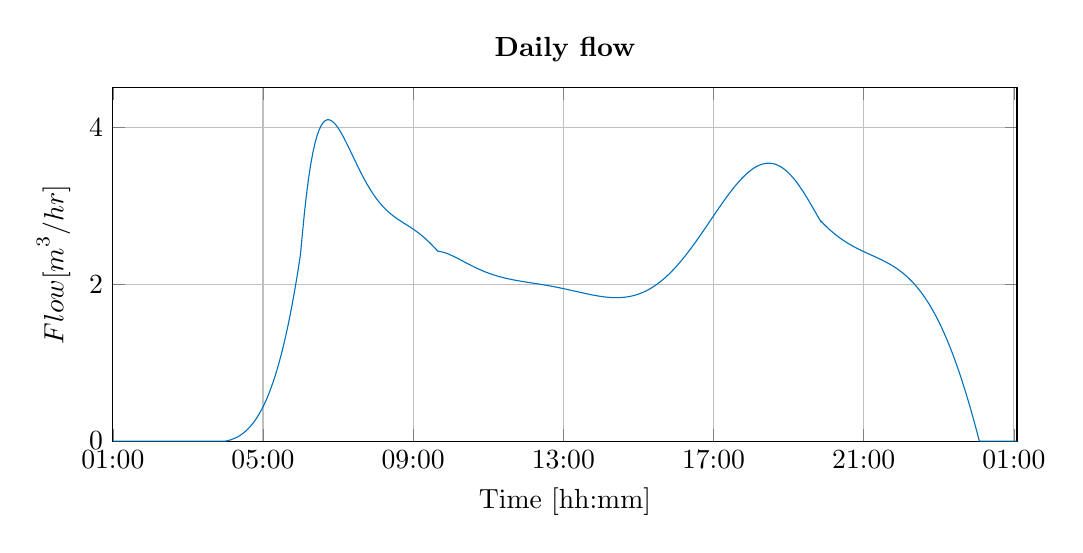
\begin{tikzpicture}

\begin{axis}[%
width=4.521in,
height=1.766in,
at={(0.758in,0.481in)},
scale only axis,
xmin=3600,
xmax=90000,
xtick={3600,17950,32300,46650,61000,75350,89700},
xticklabels={{01:00},{05:00},{09:00},{13:00},{17:00},{21:00},{01:00},{},{},{}},
xlabel={Time [hh:mm]},
xmajorgrids,
ymin=0,
ymax=4.5,
ylabel={$\text{Flow [m}^\text{3}\text{/hr]}$},
ymajorgrids,
axis background/.style={fill=white},
scaled x ticks = false,
title style={font=\bfseries},
title={Daily flow},
legend style={legend cell align=left,align=left,draw=white!15!black}
]
\addplot [color=mycolor1,solid]
  table[row sep=crcr]{%
3599	0\\
3799	0\\
3998	0\\
4197	0\\
4396	0\\
4595	0\\
4794	0\\
4993	0\\
5192	0\\
5391	0\\
5590	0\\
5789	0\\
5988	0\\
6188	0\\
6387	0\\
6586	0\\
6785	0\\
6984	0\\
7183	0\\
7382	0\\
7581	0\\
7780	0\\
7979	0\\
8178	0\\
8377	0\\
8577	0\\
8776	0\\
8975	0\\
9174	0\\
9373	0\\
9572	0\\
9771	0\\
9970	0\\
10169	0\\
10368	0\\
10567	0\\
10766	0\\
10965	0\\
11165	0\\
11364	0\\
11563	0\\
11762	0\\
11961	0\\
12160	0\\
12359	0\\
12558	0\\
12757	0\\
12956	0\\
13155	0\\
13354	0\\
13554	0\\
13753	0\\
13952	0\\
14151	0\\
14350	0\\
14549	0.00442222580352827\\
14748	0.0114741772862802\\
14947	0.0199610243832393\\
15146	0.0300247058319911\\
15345	0.0418136197449804\\
15544	0.0554826329473421\\
15743	0.0711930829844264\\
15942	0.0891127727990636\\
16142	0.109524305162895\\
16341	0.132405026798267\\
16540	0.158037982533165\\
16739	0.186616668981945\\
16938	0.218340911359329\\
17137	0.253416814139265\\
17336	0.292056704383446\\
17535	0.334479067739685\\
17734	0.380908477109851\\
17933	0.431575513987692\\
18132	0.486716682466314\\
18331	0.54657431591536\\
18531	0.61173517800162\\
18730	0.681802420108294\\
18929	0.757348375922315\\
19128	0.838637642813172\\
19327	0.925940070187446\\
19526	1.0195306221475\\
19725	1.11968923282013\\
19924	1.2267006543547\\
20123	1.34085429759121\\
20322	1.46244406539796\\
20521	1.591768178679\\
20720	1.72912899505139\\
20920	1.87558658964644\\
21119	2.02998775308587\\
21318	2.19335717408436\\
21517	2.36601181350741\\
21716	2.64411100927655\\
21915	2.91582767530568\\
22114	3.15181967017109\\
22313	3.35485836442594\\
22512	3.52758354858929\\
22711	3.67250639353341\\
22910	3.79201241085632\\
23109	3.88836441327126\\
23308	3.96370547498868\\
23508	4.02030042505377\\
23707	4.05950352712545\\
23906	4.0834448623313\\
24105	4.09381761994979\\
24175	4.0945395676626\\
24304	4.0922100675344\\
24503	4.08010851130726\\
24702	4.05890025652537\\
24901	4.02987656787424\\
25100	3.99423562983415\\
25299	3.95308550708851\\
25498	3.90744710487536\\
25697	3.85825712938731\\
25897	3.806104849663\\
26096	3.75229204330984\\
26295	3.69726553357036\\
26494	3.64165447812437\\
26693	3.58601865238405\\
26892	3.53085140987913\\
27091	3.47658264263791\\
27290	3.42358174156084\\
27489	3.37216055681841\\
27688	3.32257635822156\\
27887	3.27503479560692\\
28086	3.22969285920515\\
28285	3.18666184004508\\
28485	3.14581208430523\\
28684	3.10758088877446\\
28883	3.07174976371261\\
29082	3.03827664444324\\
29281	3.00708858386904\\
29480	2.97808471284652\\
29679	2.95113920056695\\
29878	2.92610421493529\\
30077	2.90281288295747\\
30276	2.88108225111931\\
30475	2.86071624577169\\
30674	2.84150863348836\\
30874	2.82315622926496\\
31073	2.80562396744985\\
31272	2.78859894527949\\
31471	2.77186391005839\\
31670	2.75520626611806\\
31869	2.73842103520223\\
32068	2.72131381685202\\
32267	2.70370374877641\\
32466	2.68542646722693\\
32665	2.66633706741235\\
32864	2.64631306384803\\
33063	2.62525735074963\\
33263	2.60298696876008\\
33462	2.57968708361932\\
33661	2.5552461290138\\
33860	2.52969831629012\\
34059	2.50311805326763\\
34258	2.47562290465526\\
34457	2.44737655238404\\
34656	2.41903417111451\\
34855	2.41548966232507\\
35054	2.40989498143512\\
35253	2.40252874736045\\
35452	2.39364803937087\\
35651	2.38348942106358\\
35851	2.37221122121005\\
36050	2.36012550281161\\
36249	2.34735916470061\\
36448	2.33407631847188\\
36647	2.32042527652798\\
36846	2.30653941497033\\
37045	2.292538010926\\
37244	2.27852705452525\\
37443	2.26460003586295\\
37642	2.2508387072054\\
37841	2.23731382105396\\
38040	2.22408584394744\\
38240	2.21114187463128\\
38439	2.19865344916971\\
38638	2.18658855155431\\
38837	2.17497313770969\\
39036	2.16382610120049\\
39235	2.15315984985419\\
39434	2.1429808605983\\
39633	2.13329021285326\\
39832	2.12408410098727\\
40031	2.11535432582874\\
40230	2.10708876604616\\
40429	2.09927182918011\\
40628	2.09188488312897\\
40828	2.0848725949352\\
41027	2.07828148936575\\
41226	2.07205013324472\\
41425	2.0661516594405\\
41624	2.06055803506768\\
41823	2.05524038108332\\
42022	2.0501692746057\\
42221	2.04531503405655\\
42420	2.04064798735881\\
42619	2.03613872401651\\
42818	2.03175833064229\\
43017	2.02747861102071\\
43217	2.02325129390899\\
43416	2.01909238210739\\
43615	2.01495570567951\\
43814	2.01081783906788\\
44013	2.00665694857339\\
44212	2.00245292421282\\
44411	1.99818749811514\\
44610	1.99384434968869\\
44809	1.98940919806522\\
45008	1.98486988193467\\
45207	1.98021642712068\\
45406	1.97544110247885\\
45606	1.97051349985899\\
45805	1.96547976439647\\
46004	1.96031481209514\\
46203	1.95502022754302\\
46402	1.9495999506416\\
46601	1.94406026817996\\
46800	1.93840979562937\\
46999	1.93265944979509\\
47198	1.92682241260799\\
47397	1.92091408619084\\
47596	1.91495203979398\\
47795	1.90895594880698\\
47994	1.90294752617521\\
48194	1.89692038122864\\
48393	1.89096045050175\\
48592	1.88506490030924\\
48791	1.87926277541517\\
48990	1.87358471193174\\
49189	1.86806283014049\\
49388	1.86273062200846\\
49587	1.8576228335635\\
49786	1.85277534254232\\
49985	1.84822503209959\\
50184	1.84400966023251\\
50383	1.84016772561655\\
50583	1.83672220529473\\
50782	1.83374728604262\\
50981	1.8312645559992\\
51180	1.82931407432274\\
51379	1.82793592595939\\
51578	1.82717007306889\\
51712	1.82701927855175\\
51777	1.82705620380197\\
51976	1.82763358131816\\
52175	1.82894089136547\\
52374	1.83101608970834\\
52573	1.83389624951334\\
52772	1.83761740905967\\
52971	1.84221441993455\\
53171	1.84775081767458\\
53370	1.85420339594633\\
53569	1.86162790825795\\
53768	1.8700529572691\\
53967	1.87950522064347\\
54166	1.890009309863\\
54365	1.90158763223019\\
54564	1.91426025570864\\
54763	1.92804477789214\\
54962	1.94295619853298\\
55161	1.95900679610619\\
55360	1.97620600949746\\
55560	1.9946554808804\\
55759	2.01417414547567\\
55958	2.0348515867415\\
56157	2.05668478464961\\
56356	2.07966736615765\\
56555	2.10378952045302\\
56754	2.12903792174961\\
56953	2.15539565921993\\
57152	2.18284217374636\\
57351	2.21135320365917\\
57550	2.24090073764362\\
57749	2.27145297659171\\
57949	2.30313508534694\\
58148	2.33559061425459\\
58347	2.36893225005193\\
58546	2.4031128232886\\
58745	2.43808132507356\\
58944	2.47378292667643\\
59143	2.51015901035898\\
59342	2.54714721121349\\
59541	2.58468146991496\\
59740	2.62269209826402\\
59939	2.66110585602751\\
60138	2.69984604058232\\
60337	2.73883258886069\\
60537	2.77817919271003\\
60736	2.81740559322073\\
60935	2.85661877477404\\
61134	2.89572651121671\\
61333	2.93463393237626\\
61532	2.9732437096365\\
61731	3.01145625716701\\
61930	3.04916994876029\\
62129	3.08628134942475\\
62328	3.12268546411609\\
62527	3.15827600236744\\
62726	3.19294565958974\\
62926	3.22675268320946\\
63125	3.25925012822774\\
63324	3.29050122023788\\
63523	3.32039776061185\\
63722	3.34883220757148\\
63921	3.37569806495021\\
64120	3.40089029039581\\
64319	3.42430572217504\\
64518	3.44584352561743\\
64717	3.46540566054371\\
64916	3.48289736794111\\
65115	3.49822767771618\\
65314	3.51130993772711\\
65514	3.52211038142855\\
65713	3.53044435444527\\
65912	3.53630150048119\\
66111	3.53961819236537\\
66265	3.54040515106731\\
66310	3.54033809443812\\
66509	3.53841282401017\\
66708	3.53380263676685\\
66907	3.52647713442185\\
67106	3.51641599856799\\
67305	3.50360974673538\\
67504	3.48806051398862\\
67703	3.46978285995349\\
67903	3.44869242604152\\
68102	3.42504225777269\\
68301	3.39879066106905\\
68500	3.37001054821747\\
68699	3.33879167809678\\
68898	3.30524161912064\\
69097	3.2694867393557\\
69296	3.23167322525738\\
69495	3.19196812590241\\
69694	3.15056042850421\\
69893	3.10766216016736\\
70092	3.06350951924634\\
70292	3.01813514238681\\
70491	2.97228210257935\\
70690	2.92604172777595\\
70889	2.87975895406627\\
71088	2.83380899801614\\
71260	2.79467368952501\\
71287	2.79868278125095\\
71486	2.77123878571802\\
71685	2.74481562666469\\
71884	2.71941056858078\\
72083	2.69501595485996\\
72282	2.6716193634545\\
72481	2.64920376269884\\
72680	2.6277476671415\\
72880	2.60712447469801\\
73079	2.58751035592739\\
73278	2.5687659405626\\
73477	2.55085346683633\\
73676	2.53373149886954\\
73875	2.51735508250346\\
74074	2.50167590102184\\
74273	2.4866424309576\\
74472	2.47220009798386\\
74671	2.45829143250965\\
74870	2.44485622566371\\
75069	2.43183168495778\\
75269	2.4190896353966\\
75468	2.40668971685735\\
75667	2.39449778855215\\
75866	2.38244227211082\\
76065	2.37044978534688\\
76264	2.35844529797984\\
76463	2.34635228749242\\
76662	2.33409289481071\\
76861	2.32158808022045\\
77060	2.30875777912303\\
77259	2.29552105773255\\
77458	2.28179626900046\\
77657	2.2675012083548\\
77857	2.25247636569214\\
78056	2.23678878951944\\
78255	2.22028212346615\\
78454	2.20287349134621\\
78653	2.18448023925929\\
78852	2.16502009116967\\
79051	2.14441130491532\\
79250	2.12257282778685\\
79449	2.09942445248591\\
79648	2.07488697286437\\
79847	2.04888233961291\\
80046	2.0213338162026\\
80246	1.99201534965028\\
80445	1.96114617655674\\
80644	1.92851198140894\\
80843	1.89404284661593\\
81042	1.85767094690634\\
81241	1.81933070522791\\
81440	1.77895894860465\\
81639	1.73649506384232\\
81838	1.6918811533519\\
82037	1.64506219089723\\
82236	1.59598617743537\\
82435	1.54460429694009\\
82635	1.4905950458881\\
82834	1.43445636707819\\
83033	1.37588584551451\\
83232	1.31484897432348\\
83431	1.25131520940679\\
83630	1.18525812511314\\
83829	1.11665557002792\\
84028	1.04548982286428\\
84227	0.971747748176957\\
84426	0.895420952000219\\
84625	0.816505938042502\\
84824	0.735004263003857\\
85023	0.650922692728392\\
85223	0.563831477364642\\
85422	0.474619268389663\\
85621	0.382880405254365\\
85820	0.288644077366678\\
86019	0.19194546287689\\
86218	0.0928258844168158\\
86401	0\\
86417	0\\
86616	0\\
86815	0\\
87014	0\\
87213	0\\
87412	0\\
87612	0\\
87811	0\\
88010	0\\
88209	0\\
88408	0\\
88607	0\\
88806	0\\
89005	0\\
89204	0\\
89403	0\\
89602	0\\
90000	0\\
};

\end{axis}
\end{tikzpicture}%
\caption{A daily flow profile for zone 5.}
\label{fig:APP_flow_profile_zone5}
\end{figure} 

\begin{figure}[H]
\centering
% This file was created by matlab2tikz.
%
%The latest updates can be retrieved from
%  http://www.mathworks.com/matlabcentral/fileexchange/22022-matlab2tikz-matlab2tikz
%where you can also make suggestions and rate matlab2tikz.
%
\definecolor{mycolor1}{rgb}{0.00000,0.44700,0.74100}%
%
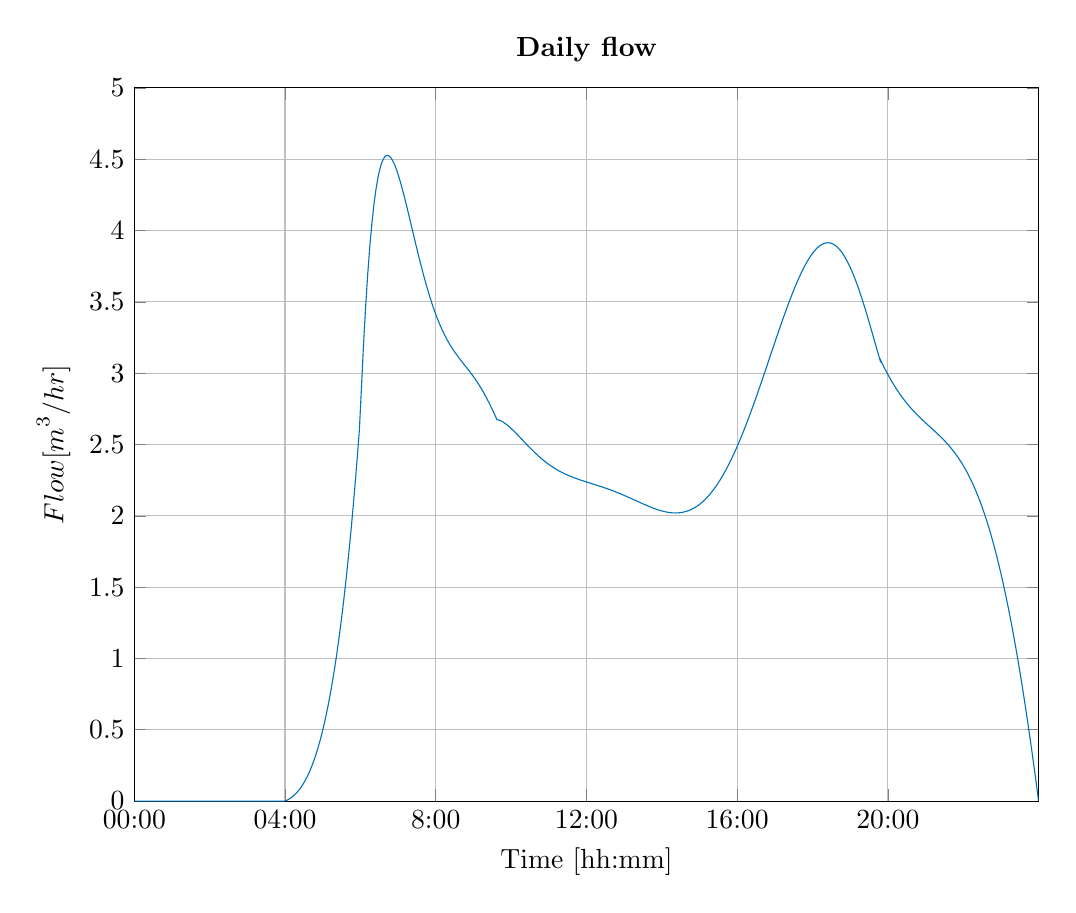
\begin{tikzpicture}

\begin{axis}[%
width=4.521in,
height=3.566in,
at={(0.758in,0.481in)},
scale only axis,
xmin=0,
xmax=24,
xtick={0,4,8,12,16,20,24},
xticklabels={{00:00},{04:00},{8:00},{12:00},{16:00},{20:00}},
xlabel={Time [hh:mm]},
xmajorgrids,
ymin=0,
ymax=5,
ylabel={$\text{Flow [m}^\text{3}\text{/hr]}$},
ymajorgrids,
axis background/.style={fill=white},
title style={font=\bfseries},
title={Daily flow}
]
\addplot [color=mycolor1,solid,forget plot]
  table[row sep=crcr]{%
0.000277777777777778	0\\
0.0558333333333333	0\\
0.111111111111111	0\\
0.166388888888889	0\\
0.221666666666667	0\\
0.276944444444444	0\\
0.332222222222222	0\\
0.3875	0\\
0.442777777777778	0\\
0.498055555555556	0\\
0.553333333333333	0\\
0.608611111111111	0\\
0.663888888888889	0\\
0.719166666666667	0\\
0.774722222222222	0\\
0.83	0\\
0.885277777777778	0\\
0.940555555555556	0\\
0.995833333333333	0\\
1.05111111111111	0\\
1.10638888888889	0\\
1.16166666666667	0\\
1.21694444444444	0\\
1.27222222222222	0\\
1.3275	0\\
1.38277777777778	0\\
1.43805555555556	0\\
1.49361111111111	0\\
1.54888888888889	0\\
1.60416666666667	0\\
1.65944444444444	0\\
1.71472222222222	0\\
1.77	0\\
1.82527777777778	0\\
1.88055555555556	0\\
1.93583333333333	0\\
1.99111111111111	0\\
2.04638888888889	0\\
2.10166666666667	0\\
2.15694444444444	0\\
2.2125	0\\
2.26777777777778	0\\
2.32305555555556	0\\
2.37833333333333	0\\
2.43361111111111	0\\
2.48888888888889	0\\
2.54416666666667	0\\
2.59944444444444	0\\
2.65472222222222	0\\
2.71	0\\
2.76527777777778	0\\
2.82055555555556	0\\
2.87583333333333	0\\
2.93138888888889	0\\
2.98666666666667	0\\
3.04194444444444	0\\
3.09722222222222	0\\
3.1525	0\\
3.20777777777778	0\\
3.26305555555556	0\\
3.31833333333333	0\\
3.37361111111111	0\\
3.42888888888889	0\\
3.48416666666667	0\\
3.53944444444444	0\\
3.59472222222222	0\\
3.65027777777778	0\\
3.70555555555556	0\\
3.76083333333333	0\\
3.81611111111111	0\\
3.87138888888889	0\\
3.92666666666667	0\\
3.98194444444444	0\\
4.03722222222222	0.00436153761647452\\
4.0925	0.012044686962592\\
4.14777777777778	0.0213027030151159\\
4.20305555555556	0.0322919741793307\\
4.25833333333333	0.0451760291745809\\
4.31361111111111	0.0601255479688758\\
4.36916666666667	0.0774107346184819\\
4.42444444444444	0.0970445135396201\\
4.47972222222222	0.119299674842479\\
4.535	0.14437548643156\\
4.59027777777778	0.172478300400132\\
4.64555555555556	0.203821515298544\\
4.70083333333333	0.238625530298273\\
4.75611111111111	0.27711769125169\\
4.81138888888889	0.319532228647551\\
4.86666666666667	0.366110187462214\\
4.92194444444444	0.417099348906629\\
4.97722222222222	0.472754144068967\\
5.0325	0.533335559453085\\
5.08777777777778	0.599111034412647\\
5.14333333333333	0.670726634405299\\
5.19861111111111	0.747747397579227\\
5.25388888888889	0.830803561132116\\
5.30916666666667	0.920187217675859\\
5.36444444444444	1.01619627753933\\
5.41972222222222	1.11913431753617\\
5.475	1.22931042162831\\
5.53027777777778	1.34703901348522\\
5.58555555555556	1.47263968093894\\
5.64083333333333	1.60643699233471\\
5.69611111111111	1.74876030477746\\
5.75138888888889	1.89994356427397\\
5.80666666666667	2.06032509777082\\
5.86222222222222	2.23112595329756\\
5.9175	2.41098601653716\\
5.97277777777778	2.60108518753465\\
6.02805555555556	2.89896921282579\\
6.08333333333333	3.20248193836858\\
6.13861111111111	3.46626088004164\\
6.19388888888889	3.69338113557894\\
6.24916666666667	3.88677208244\\
6.30444444444444	4.04922065076256\\
6.35972222222222	4.18337459634552\\
6.415	4.29174577360512\\
6.47027777777778	4.37671340855667\\
6.52555555555556	4.4405273717661\\
6.58111111111111	4.48549187067167\\
6.63638888888889	4.51316632254109\\
6.69166666666667	4.52570246958311\\
6.71527777777778	4.52688225493132\\
6.74694444444444	4.52486491431809\\
6.80222222222222	4.5123052851202\\
6.8575	4.48956550917361\\
6.91277777777778	4.45808108545889\\
6.96805555555556	4.41918435771153\\
7.02333333333333	4.3741077873827\\
7.07861111111111	4.32398722662112\\
7.13388888888889	4.26986519123494\\
7.18916666666667	4.21269413366429\\
7.24444444444444	4.15333971595018\\
7.3	4.09227645710956\\
7.35527777777778	4.03081963544181\\
7.41055555555556	3.96929137850569\\
7.46583333333333	3.90824255434165\\
7.52111111111111	3.84815362185813\\
7.57638888888889	3.78943790384718\\
7.63166666666667	3.73244485989398\\
7.68694444444444	3.67746335940641\\
7.74222222222222	3.62472495453506\\
7.7975	3.5744071531644\\
7.85277777777778	3.52663669187815\\
7.90805555555556	3.48149280893884\\
7.96333333333333	3.43901051721824\\
8.01888888888889	3.39899039075237\\
8.07416666666667	3.36178873974155\\
8.12944444444445	3.32712062267076\\
8.18472222222222	3.29487673247597\\
8.24	3.26491991800917\\
8.29527777777778	3.23708845702013\\
8.35055555555556	3.21119932911955\\
8.40583333333333	3.18705148874919\\
8.46111111111111	3.16442913815202\\
8.51638888888889	3.14310500034235\\
8.57166666666667	3.1228435920573\\
8.62694444444444	3.10340449676192\\
8.68222222222222	3.08454563756568\\
8.73777777777778	3.06593394703847\\
8.79305555555556	3.04751899406006\\
8.84833333333333	3.02897969760621\\
8.90361111111111	3.01010013488272\\
8.95888888888889	2.99067910406758\\
9.01416666666667	2.97053339725773\\
9.06944444444444	2.94950107348585\\
9.12472222222222	2.92744473160188\\
9.18	2.9042547833318\\
9.23527777777778	2.87985272619639\\
9.29055555555555	2.85419441649543\\
9.34583333333333	2.82727334224515\\
9.40111111111111	2.79912389620901\\
9.45666666666667	2.76967470488772\\
9.51194444444444	2.73934693504096\\
9.56722222222222	2.70817315136422\\
9.6225	2.67465448833025\\
9.67777777777778	2.67091974484706\\
9.73305555555556	2.66489413494212\\
9.78833333333333	2.65688753866974\\
9.84361111111111	2.64718593550291\\
9.89888888888889	2.63605253876402\\
9.95416666666667	2.62372889951666\\
10.0094444444444	2.61043598011424\\
10.0647222222222	2.59637519806299\\
10.12	2.58172944029236\\
10.1752777777778	2.56666404826203\\
10.2308333333333	2.55125025460983\\
10.2861111111111	2.53577580856133\\
10.3413888888889	2.52028246107213\\
10.3966666666667	2.50487458576866\\
10.4519444444444	2.48964351667202\\
10.5072222222222	2.47466836579301\\
10.5625	2.46001681462221\\
10.6177777777778	2.44574587907216\\
10.6730555555556	2.43190264870155\\
10.7283333333333	2.41852500035662\\
10.7836111111111	2.40564228683593\\
10.8388888888889	2.39327600059714\\
10.8941666666667	2.38144041312116\\
10.9497222222222	2.37008778498997\\
11.005	2.35933328724769\\
11.0602777777778	2.34911498058241\\
11.1155555555556	2.3394241478704\\
11.1708333333333	2.33024769699801\\
11.2261111111111	2.32156866154641\\
11.2813888888889	2.3133666791386\\
11.3366666666667	2.30561844877292\\
11.3919444444444	2.29829816650414\\
11.4472222222222	2.291377940787\\
11.5025	2.28482818722587\\
11.5577777777778	2.27861800322458\\
11.6130555555556	2.27271552299811\\
11.6686111111111	2.2670606152517\\
11.7238888888889	2.26167688742547\\
11.7791666666667	2.25650258532945\\
11.8344444444444	2.25150516187116\\
11.8897222222222	2.24665260063167\\
11.945	2.24191366027968\\
12.0002777777778	2.23725810189779\\
12.0555555555556	2.23265689961728\\
12.1108333333333	2.2280824345194\\
12.1661111111111	2.22350867287552\\
12.2213888888889	2.2189113285537\\
12.2766666666667	2.21426800980611\\
12.3319444444444	2.20955835157951\\
12.3875	2.20473980000995\\
12.4427777777778	2.1998445059343\\
12.4980555555556	2.19483497865375\\
12.5533333333333	2.1897000062789\\
12.6086111111111	2.18443085250946\\
12.6638888888889	2.17902130650358\\
12.7191666666667	2.17346772034056\\
12.7744444444444	2.16776903444503\\
12.8297222222222	2.16192679117337\\
12.885	2.15594513737332\\
12.9402777777778	2.14983081564193\\
12.9955555555556	2.14359314511635\\
13.0508333333333	2.13724399207717\\
13.1063888888889	2.13076511965299\\
13.1616666666667	2.1242382262651\\
13.2169444444444	2.11765039444991\\
13.2722222222222	2.11102320411836\\
13.3275	2.10438049385537\\
13.3827777777778	2.09774827749962\\
13.4380555555556	2.09115465352914\\
13.4933333333333	2.08462970606388\\
13.5486111111111	2.07820540021266\\
13.6038888888889	2.07191546984384\\
13.6591666666667	2.06579529944379\\
13.7144444444444	2.05988180019883\\
13.7697222222222	2.05421328036551\\
13.8252777777778	2.04880304224001\\
13.8805555555556	2.04374605492379\\
13.9358333333333	2.0390561953673\\
13.9911111111111	2.03477597078221\\
14.0463888888889	2.03094856698806\\
14.1016666666667	2.02761769324186\\
14.1569444444444	2.02482742427944\\
14.2122222222222	2.02262203963405\\
14.2675	2.02104586064697\\
14.3227777777778	2.02014308607478\\
14.3644444444444	2.01993435765349\\
14.3780555555556	2.01995762529078\\
14.4333333333333	2.02053293136058\\
14.4886111111111	2.02191183224794\\
14.5438888888889	2.02413636276678\\
14.5994444444444	2.02726553651458\\
14.6547222222222	2.03130816790608\\
14.71	2.03631627688364\\
14.7652777777778	2.04232703369705\\
14.8205555555556	2.04937597715924\\
14.8758333333333	2.0574968510835\\
14.9311111111111	2.0667214424411\\
14.9863888888889	2.07707942275923\\
15.0416666666667	2.08859819167305\\
15.0969444444444	2.10130272383475\\
15.1522222222222	2.11521541959434\\
15.2075	2.13035595966703\\
15.2627777777778	2.1467411634931\\
15.3183333333333	2.16447671199407\\
15.3736111111111	2.1833959789767\\
15.4288888888889	2.20359189061787\\
15.4841666666667	2.22506849094935\\
15.5394444444444	2.24782633363513\\
15.5947222222222	2.27186237375637\\
15.65	2.29716986664122\\
15.7052777777778	2.32373827452759\\
15.7605555555556	2.35155318020554\\
15.8158333333333	2.38059620817089\\
15.8711111111111	2.41084495540202\\
15.9263888888889	2.44227292966191\\
15.9816666666667	2.47484949673807\\
16.0372222222222	2.50871188458511\\
16.0925	2.54348225841157\\
16.1477777777778	2.57928386421897\\
16.2030555555556	2.61606914921719\\
16.2583333333333	2.65378630529219\\
16.3136111111111	2.69237927794856\\
16.3688888888889	2.73178778774273\\
16.4241666666667	2.77194736275682\\
16.4794444444444	2.81278938394544\\
16.5347222222222	2.85424114271212\\
16.59	2.8962259122492\\
16.6452777777778	2.9386630310047\\
16.7005555555556	2.98146800095245\\
16.7561111111111	3.02476965789499\\
16.8113888888889	3.06804277125561\\
16.8666666666667	3.11140792872131\\
16.9219444444444	3.15476653670328\\
16.9772222222222	3.19801687465371\\
17.0325	3.24105428237435\\
17.0877777777778	3.28377136503771\\
17.1430555555556	3.32605821353838\\
17.1983333333333	3.36780264295779\\
17.2536111111111	3.40889044762271\\
17.3088888888889	3.44920567419794\\
17.3641666666667	3.4886309126315\\
17.4194444444444	3.52704760641628\\
17.475	3.56452071052627\\
17.5302777777778	3.60055514510756\\
17.5855555555556	3.63522126139752\\
17.6408333333333	3.66839939552844\\
17.6961111111111	3.6999705763583\\
17.7513888888889	3.72981695353354\\
17.8066666666667	3.75782224692899\\
17.8619444444444	3.78387221647664\\
17.9172222222222	3.80785515508745\\
17.9725	3.82966240233964\\
18.0277777777778	3.84918888157241\\
18.0830555555556	3.86633365900495\\
18.1383333333333	3.88100052684839\\
18.1938888888889	3.89315277138449\\
18.2491666666667	3.90258361670261\\
18.3044444444444	3.9092820912385\\
18.3597222222222	3.91317723245379\\
18.4069444444444	3.91423675086944\\
18.415	3.91420608156746\\
18.4702777777778	3.91231441194926\\
18.5255555555556	3.90745748655999\\
18.5808333333333	3.89960083715605\\
18.6361111111111	3.88872107271818\\
18.6913888888889	3.87480671522994\\
18.7466666666667	3.85785905987809\\
18.8019444444444	3.83789306517646\\
18.8572222222222	3.81493827049557\\
18.9127777777778	3.78890226035816\\
18.9680555555556	3.760107261838\\
19.0233333333333	3.72850960520155\\
19.0786111111111	3.69420699034698\\
19.1338888888889	3.65731672045863\\
19.1891666666667	3.61797679517985\\
19.2444444444444	3.57634703184434\\
19.2997222222222	3.53261022120022\\
19.355	3.48697331026012\\
19.4102777777778	3.43966862035264\\
19.4655555555556	3.39095509469634\\
19.5208333333333	3.34111957862943\\
19.5761111111111	3.29047813315719\\
19.6313888888889	3.23937738191039\\
19.6869444444444	3.18793917311625\\
19.7422222222222	3.13709162073664\\
19.7944444444444	3.08976345798418\\
19.7975	3.09668439391876\\
19.8527777777778	3.06625187787283\\
19.9080555555556	3.03694799011631\\
19.9633333333333	3.00877015128834\\
20.0186111111111	2.98171032737234\\
20.0738888888889	2.95575520193564\\
20.1291666666667	2.93088634834114\\
20.1844444444444	2.90708040194028\\
20.2397222222222	2.88430923245258\\
20.295	2.86254011607467\\
20.3502777777778	2.84173590774791\\
20.4058333333333	2.82175756742555\\
20.4611111111111	2.8027592071145\\
20.5163888888889	2.78458925699978\\
20.5716666666667	2.76719459119578\\
20.6269444444444	2.75051852452434\\
20.6822222222222	2.73450098492227\\
20.7375	2.71907868568098\\
20.7927777777778	2.70418529751819\\
20.8480555555556	2.68975162102279\\
20.9033333333333	2.67570575874519\\
20.9586111111111	2.66197328747429\\
21.0138888888889	2.64847743056102\\
21.0691666666667	2.63513922997144\\
21.1247222222222	2.62181113258648\\
21.18	2.60854326423953\\
21.2352777777778	2.59518438463777\\
21.2905555555556	2.58164852618859\\
21.3458333333333	2.56784840185863\\
21.4011111111111	2.55369557773978\\
21.4563888888889	2.53910064522353\\
21.5116666666667	2.52397339311935\\
21.5669444444444	2.50822298001557\\
21.6222222222222	2.49175810653765\\
21.6775	2.4744871874106\\
21.7327777777778	2.4563185239504\\
21.7880555555556	2.43716047605184\\
21.8436111111111	2.41681704892677\\
21.8988888888889	2.39540029069326\\
21.9541666666667	2.3727208498224\\
22.0094444444444	2.34868904762022\\
22.0647222222222	2.32321612616745\\
22.12	2.29621442048452\\
22.1752777777778	2.26759753094839\\
22.2305555555556	2.23728049530837\\
22.2858333333333	2.20517996105627\\
22.3411111111111	2.17121435762874\\
22.3963888888889	2.13530406869352\\
22.4516666666667	2.09737160427715\\
22.5069444444444	2.05734177313516\\
22.5625	2.01492419568342\\
22.6177777777778	1.97047268369193\\
22.6730555555556	1.92371341495077\\
22.7283333333333	1.8745821306619\\
22.7836111111111	1.82301773275629\\
22.8388888888889	1.76896245618956\\
22.8941666666667	1.71236204108829\\
22.9494444444444	1.65316590500831\\
23.0047222222222	1.59132731520234\\
23.06	1.52680356080361\\
23.1152777777778	1.45955612515875\\
23.1705555555556	1.38955085797417\\
23.2258333333333	1.31675814765827\\
23.2813888888889	1.2407660309182\\
23.3366666666667	1.16231433996367\\
23.3919444444444	1.08101526302932\\
23.4472222222222	0.996859091977158\\
23.5025	0.909841519641678\\
23.5577777777778	0.81996381149129\\
23.6130555555556	0.727232978502056\\
23.6683333333333	0.631661948660645\\
23.7236111111111	0.533269739987247\\
23.7788888888889	0.432081632122456\\
23.8341666666667	0.328129339023808\\
23.8894444444444	0.221451180851064\\
23.9447222222222	0.112092256448278\\
24	0.000104615546122659\\
};
\end{axis}
\end{tikzpicture}%
\caption{A daily flow profile for zone 6.}
\label{fig:APP_flow_profile_zone6}
\end{figure} 

\begin{figure}[H]
\centering
% This file was created by matlab2tikz.
%
%The latest updates can be retrieved from
%  http://www.mathworks.com/matlabcentral/fileexchange/22022-matlab2tikz-matlab2tikz
%where you can also make suggestions and rate matlab2tikz.
%
\definecolor{mycolor1}{rgb}{0.00000,0.44700,0.74100}%
\definecolor{mycolor2}{rgb}{0.85000,0.32500,0.09800}%
%
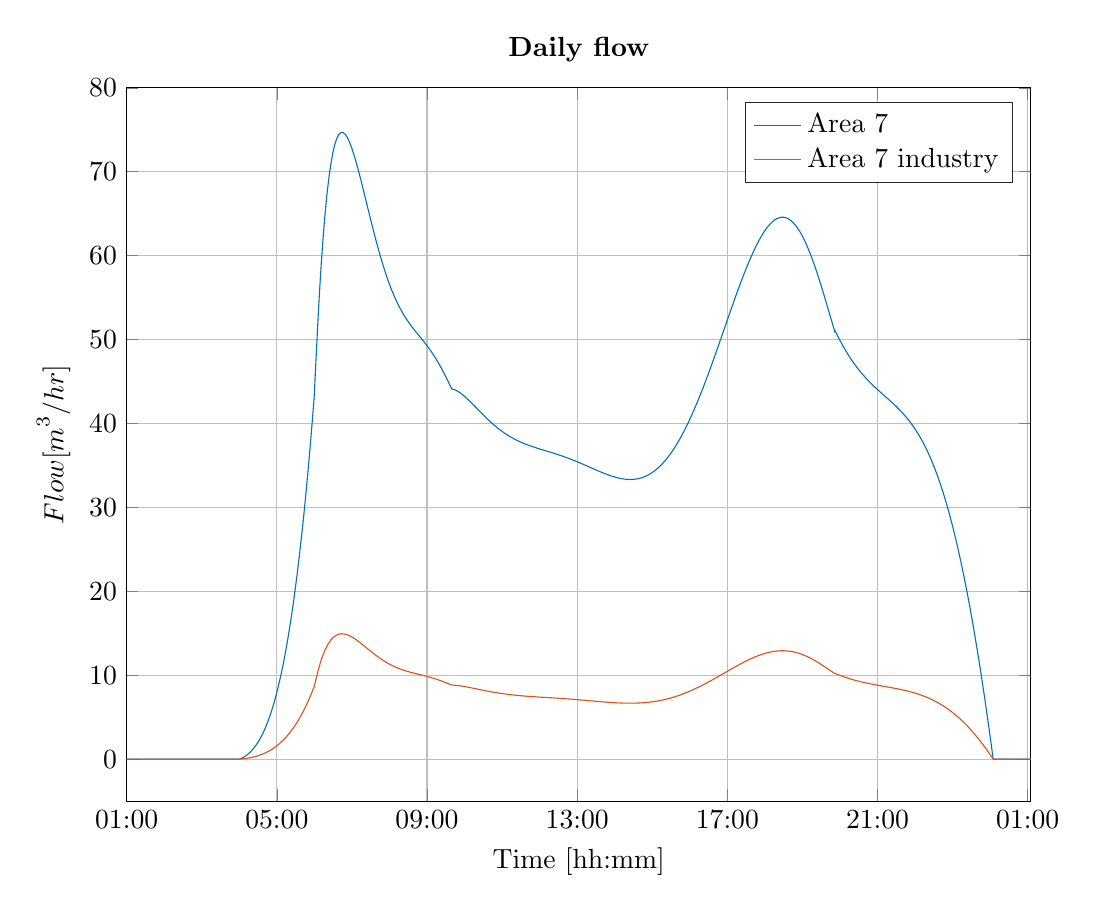
\begin{tikzpicture}

\begin{axis}[%
width=4.521in,
height=3.566in,
at={(0.758in,0.481in)},
scale only axis,
xmin=3600,
xmax=90000,
xtick={3600,17950,32300,46650,61000,75350,89700},
xticklabels={{01:00},{05:00},{09:00},{13:00},{17:00},{21:00},{01:00},{},{},{}},
xlabel={Time [hh:mm]},
xmajorgrids,
ymin=-5,
ymax=80,
ylabel={$\text{Flow [m}^\text{3}\text{/hr]}$},
scaled x ticks = false,
ymajorgrids,
axis background/.style={fill=white},
title style={font=\bfseries},
title={Daily flow},
legend style={legend cell align=left,align=left,draw=white!15!black}
]
\addplot [color=mycolor1,solid]
  table[row sep=crcr]{%
3599	0\\
3799	0\\
3998	0\\
4197	0\\
4396	0\\
4595	0\\
4794	0\\
4993	0\\
5192	0\\
5391	0\\
5590	0\\
5789	0\\
5988	0\\
6188	0\\
6387	0\\
6586	0\\
6785	0\\
6984	0\\
7183	0\\
7382	0\\
7581	0\\
7780	0\\
7979	0\\
8178	0\\
8377	0\\
8577	0\\
8776	0\\
8975	0\\
9174	0\\
9373	0\\
9572	0\\
9771	0\\
9970	0\\
10169	0\\
10368	0\\
10567	0\\
10766	0\\
10965	0\\
11165	0\\
11364	0\\
11563	0\\
11762	0\\
11961	0\\
12160	0\\
12359	0\\
12558	0\\
12757	0\\
12956	0\\
13155	0\\
13354	0\\
13554	0\\
13753	0\\
13952	0\\
14151	0\\
14350	0\\
14549	0.0806712868631212\\
14748	0.209314650247236\\
14947	0.364133718096731\\
15146	0.547717770363713\\
15345	0.76277392044104\\
15544	1.01212728550524\\
15743	1.29872102313826\\
15942	1.62561623422888\\
16142	1.99796822523865\\
16341	2.41536374972987\\
16540	2.88296617826028\\
16739	3.40430532173897\\
16938	3.98302643889659\\
17137	4.62288933619267\\
17336	5.32776733400112\\
17535	6.10164609907736\\
17734	6.94862234330207\\
17933	7.87290238870716\\
18132	8.87880059877989\\
18331	9.97073767604603\\
18531	11.1594175018059\\
18730	12.4376006699258\\
18929	13.8157278266077\\
19128	15.2986258195173\\
19327	16.8912173052207\\
19526	18.5985182437715\\
19725	20.4256352595821\\
19924	22.37776286857\\
20123	24.4601805715863\\
20322	26.678249814123\\
20521	29.0374108122996\\
20720	31.5431792451301\\
20920	34.214893253364\\
21119	37.0315157193367\\
21318	40.0117392564332\\
21517	43.1613459395731\\
21716	48.2344971071132\\
21915	53.1912166607005\\
22114	57.4962383310093\\
22313	61.2001181137826\\
22512	64.3510116907251\\
22711	66.9947284335877\\
22910	69.1747854079815\\
23109	70.9324613775012\\
23308	72.3068508077128\\
23508	73.3392692446144\\
23707	74.0544214855121\\
23906	74.4911649730871\\
24105	74.6803872657921\\
24175	74.6935572063667\\
24304	74.6510619152082\\
24503	74.4303024702448\\
24702	74.0434164808385\\
24901	73.5139595021531\\
25100	72.8637890982789\\
25299	72.1131188467016\\
25498	71.2805723417324\\
25697	70.3832371988232\\
25897	69.4318630028585\\
26096	68.4501970882049\\
26295	67.4463905099139\\
26494	66.4319205108774\\
26693	65.4169986462854\\
26892	64.4106247876708\\
27091	63.4206411268791\\
27290	62.4537861799018\\
27489	61.5157487911532\\
27688	60.6112221372467\\
27887	59.7439577310406\\
28086	58.9168194253759\\
28285	58.1318374174683\\
28485	57.3866465317048\\
28684	56.6892240393205\\
28883	56.0355841989065\\
29082	55.4249596567068\\
29281	54.8560196945552\\
29480	54.3269242337281\\
29679	53.8353778389139\\
29878	53.3786837221425\\
30077	52.9537977468702\\
30276	52.5573824319095\\
30475	52.1858609554749\\
30674	51.8354711587287\\
30874	51.500682269262\\
31073	51.1808546111814\\
31272	50.8702801384215\\
31471	50.5649956760341\\
31670	50.2611230036569\\
31869	49.9549228595587\\
32068	49.6428489446855\\
32267	49.3216019264368\\
32466	48.9881834425187\\
32665	48.6399501055283\\
32864	48.2746675063458\\
33063	47.8905642183332\\
33263	47.4843026537165\\
33462	47.0592606496269\\
33661	46.6134029870405\\
33860	46.1473537574166\\
34059	45.6624703257579\\
34258	45.1608973352329\\
34457	44.6456207102605\\
34656	44.1285923016355\\
34855	44.0639325357064\\
35054	43.9618730464282\\
35253	43.8274964658239\\
35452	43.6654924946103\\
35651	43.4801765817624\\
35851	43.2744369980988\\
36050	43.0539664705448\\
36249	42.8210799175509\\
36448	42.5787711015646\\
36647	42.329745572439\\
36846	42.0764364084961\\
37045	41.8210194912402\\
37244	41.5654283176438\\
37443	41.3113683560837\\
37642	41.0603309506973\\
37841	40.8136067853135\\
38040	40.5722989048051\\
38240	40.3361719614414\\
38439	40.1083551565928\\
38638	39.888264446677\\
38837	39.6763733257973\\
39036	39.4730264548188\\
39235	39.2784501802593\\
39434	39.092762655759\\
39633	38.9159835723603\\
39832	38.7480435068298\\
40031	38.5887928879442\\
40230	38.4380105955128\\
40429	38.295412188211\\
40628	38.1606577748434\\
40828	38.0327379585383\\
41027	37.9125014550759\\
41226	37.7988275859611\\
41425	37.6912262346382\\
41624	37.5891860185948\\
41823	37.4921801195138\\
42022	37.3996717982419\\
42221	37.3111195964229\\
42420	37.2259822290237\\
42619	37.1437231828353\\
42818	37.0638150130212\\
43017	36.9857433575641\\
43217	36.9086276410602\\
43416	36.8327597903689\\
43615	36.7572975626132\\
43814	36.6818136232444\\
44013	36.6059096767705\\
44212	36.5292188721308\\
44411	36.4514079625103\\
44610	36.3721792238241\\
44809	36.2912721411028\\
45008	36.2084648648579\\
45207	36.1235754438101\\
45406	36.0364628445986\\
45606	35.9465723545705\\
45805	35.8547457641767\\
46004	35.7605254852387\\
46203	35.6639404241854\\
46402	35.5650624536297\\
46601	35.4640062586617\\
46800	35.3609290047419\\
46999	35.2560298388086\\
47198	35.1495492287557\\
47397	35.0417681437422\\
47596	34.9330070861796\\
47795	34.8236249791683\\
47994	34.7140179153825\\
48194	34.6040693147113\\
48393	34.4953468516997\\
48592	34.3877988335915\\
48791	34.2819551018283\\
48990	34.1783745275995\\
49189	34.0776430566623\\
49388	33.9803716573841\\
49587	33.8871941750062\\
49786	33.7987650996695\\
49985	33.7157572625869\\
50184	33.6388594540552\\
50383	33.5687739759988\\
50583	33.5059199810597\\
50782	33.451650801908\\
50981	33.4063602544698\\
51180	33.3707791073658\\
51379	33.3456385996443\\
51578	33.3316677304554\\
51712	33.3289169012826\\
51777	33.3295905004124\\
51976	33.3401231573381\\
52175	33.3639714157788\\
52374	33.4018276737478\\
52573	33.4543682286999\\
52772	33.5222504994301\\
52971	33.6061102568185\\
53171	33.7071065311195\\
53370	33.8248159869216\\
53569	33.9602556928795\\
53768	34.1139474254617\\
53967	34.2863778449061\\
54166	34.4779959196747\\
54365	34.6892104090688\\
54564	34.9203873976167\\
54763	35.1718479047777\\
54962	35.4438655595737\\
55161	35.7366643488439\\
55360	36.0504164589691\\
55560	36.3869760704703\\
55759	36.743040156907\\
55958	37.1202429208683\\
56157	37.5185292702852\\
56356	37.937782946615\\
56555	38.3778249786989\\
56754	38.8384122744013\\
56953	39.3192363424157\\
57152	39.8199221384663\\
57351	40.3400270754471\\
57550	40.8790401643436\\
57749	41.4363813183221\\
57949	42.0143338239998\\
58148	42.6063952426442\\
58347	43.2146212323138\\
58546	43.8381513167616\\
58745	44.4760549797581\\
58944	45.1273320226626\\
59143	45.7909131268592\\
59342	46.4656606169815\\
59541	47.1503694232313\\
59740	47.8437682770275\\
59939	48.5445211127502\\
60138	49.2512287030452\\
60337	49.9624305185332\\
60537	50.6802005527289\\
60736	51.3957778092502\\
60935	52.1111139224308\\
61134	52.8245264810153\\
61333	53.5342848409259\\
61532	54.2386135105739\\
61731	54.9356958217361\\
61930	55.6236778851489\\
62129	56.3006728152825\\
62328	56.9647652677576\\
62527	57.61401626679\\
62726	58.2464683367395\\
62926	58.863184040908\\
63125	59.4560101031359\\
63324	60.0260998996189\\
63523	60.5714796454472\\
63722	61.0901875381207\\
63921	61.5802808494333\\
64120	62.039843372003\\
64319	62.4669932051434\\
64518	62.8598908989963\\
64717	63.2167479814712\\
64916	63.5358358362923\\
65115	63.8154949655431\\
65314	64.0541446404007\\
65514	64.2511688835754\\
65713	64.4031991863712\\
65912	64.5100466267904\\
66111	64.5705505029634\\
66265	64.5849063893458\\
66310	64.5836831264892\\
66509	64.5485618889309\\
66708	64.4644617651194\\
66907	64.3308282223415\\
67106	64.1472906074174\\
67305	63.9136759388932\\
67504	63.6300231651217\\
67703	63.2965978862322\\
67903	62.9118612129437\\
68102	62.4804292613564\\
68301	62.0015414382595\\
68500	61.4765278267994\\
68699	60.9070258296289\\
68898	60.2949977351386\\
69097	59.6427487794266\\
69296	58.9529457303162\\
69495	58.228635936493\\
69694	57.4732669473098\\
69893	56.6907066112517\\
70092	55.8852637144502\\
70292	55.0575336222985\\
70491	54.2210716476743\\
70690	53.3775438166332\\
70889	52.5332425347369\\
71088	51.6950125911392\\
71260	50.9810970567389\\
71287	51.0542318542487\\
71486	50.5535920102722\\
71685	50.0715745062993\\
71884	49.6081294405078\\
72083	49.1631171392776\\
72282	48.7363109966823\\
72481	48.3274003170589\\
72680	47.9359931577304\\
72880	47.5597800135905\\
73079	47.2019746295574\\
73278	46.8600345803252\\
73477	46.5332710068217\\
73676	46.2209280259618\\
73875	45.9221855733706\\
74074	45.6361622441064\\
74273	45.3619181349223\\
74472	45.0984576880658\\
74671	44.8447325296946\\
74870	44.5996443153685\\
75069	44.3620475696956\\
75269	44.1296040941603\\
75468	43.9034018534785\\
75667	43.680993819737\\
75866	43.4610742434129\\
76065	43.2423044693403\\
76264	43.0233157774334\\
76463	42.802712225871\\
76662	42.5790734910501\\
76861	42.3509577118476\\
77060	42.1169043309587\\
77259	41.8754369351584\\
77458	41.6250660997165\\
77657	41.3642922294289\\
77857	41.0902055033405\\
78056	40.8040290361404\\
78255	40.5029105380129\\
78454	40.1853381620114\\
78653	39.8498041161772\\
78852	39.4948075016479\\
79051	39.1188571586106\\
79250	38.7204745044099\\
79449	38.2981963785783\\
79648	37.8505778838674\\
79847	37.3761952263548\\
80046	36.8736485601679\\
80246	36.3388141734341\\
80445	35.7756914319698\\
80644	35.1803707416029\\
80843	34.5515766491365\\
81042	33.8880718699623\\
81241	33.1886601320148\\
81440	32.4521890189557\\
81639	31.6775528105893\\
81838	30.8636953254318\\
82037	30.0096127618954\\
82236	29.1143565411657\\
82435	28.1770361497705\\
82635	27.1917866445549\\
82834	26.1676916155817\\
83033	25.0992343371187\\
83232	23.9857853266339\\
83431	22.8267873914767\\
83630	21.6217584686788\\
83829	20.3702944669068\\
84028	19.0720721102633\\
84227	17.7268517788554\\
84426	16.3344803479791\\
84625	14.8948940374586\\
84824	13.4081212449834\\
85023	11.8742853946788\\
85223	10.2855468883227\\
85422	8.65811671590336\\
85621	6.98459472193833\\
85820	5.26551338649648\\
86019	3.5015144376983\\
86218	1.69335169274651\\
86401	0\\
86417	0\\
86616	0\\
86815	0\\
87014	0\\
87213	0\\
87412	0\\
87612	0\\
87811	0\\
88010	0\\
88209	0\\
88408	0\\
88607	0\\
88806	0\\
89005	0\\
89204	0\\
89403	0\\
89602	0\\
90000	0\\
};
\addlegendentry{Area 7};

\addplot [color=mycolor2,solid]
  table[row sep=crcr]{%
3599	0\\
3799	0\\
3998	0\\
4197	0\\
4396	0\\
4595	0\\
4794	0\\
4993	0\\
5192	0\\
5391	0\\
5590	0\\
5789	0\\
5988	0\\
6188	0\\
6387	0\\
6586	0\\
6785	0\\
6984	0\\
7183	0\\
7382	0\\
7581	0\\
7780	0\\
7979	0\\
8178	0\\
8377	0\\
8577	0\\
8776	0\\
8975	0\\
9174	0\\
9373	0\\
9572	0\\
9771	0\\
9970	0\\
10169	0\\
10368	0\\
10567	0\\
10766	0\\
10965	0\\
11165	0\\
11364	0\\
11563	0\\
11762	0\\
11961	0\\
12160	0\\
12359	0\\
12558	0\\
12757	0\\
12956	0\\
13155	0\\
13354	0\\
13554	0\\
13753	0\\
13952	0\\
14151	0\\
14350	0\\
14549	0.0161342573726242\\
14748	0.0418629300494472\\
14947	0.0728267436193462\\
15146	0.109543554072743\\
15345	0.152554784088208\\
15544	0.202425457101048\\
15743	0.259744204627653\\
15942	0.325123246845776\\
16142	0.399593645047731\\
16341	0.483072749945975\\
16540	0.576593235652055\\
16739	0.680861064347794\\
16938	0.796605287779317\\
17137	0.924577867238534\\
17336	1.06555346680022\\
17535	1.22032921981547\\
17734	1.38972446866041\\
17933	1.57458047774143\\
18132	1.77576011975598\\
18331	1.99414753520921\\
18531	2.23188350036119\\
18730	2.48752013398517\\
18929	2.76314556532154\\
19128	3.05972516390346\\
19327	3.37824346104413\\
19526	3.71970364875431\\
19725	4.08512705191643\\
19924	4.47555257371399\\
20123	4.89203611431725\\
20322	5.3356499628246\\
20521	5.80748216245992\\
20720	6.30863584902602\\
20920	6.8429786506728\\
21119	7.40630314386734\\
21318	8.00234785128665\\
21517	8.63226918791462\\
21716	9.64689942142263\\
21915	10.6382433321401\\
22114	11.4992476662019\\
22313	12.2400236227565\\
22512	12.870202338145\\
22711	13.3989456867175\\
22910	13.8349570815963\\
23109	14.1864922755002\\
23308	14.4613701615426\\
23508	14.6678538489229\\
23707	14.8108842971024\\
23906	14.8982329946174\\
24105	14.9360774531584\\
24175	14.9387114412733\\
24304	14.9302123830416\\
24503	14.886060494049\\
24702	14.8086832961677\\
24901	14.7027919004306\\
25100	14.5727578196558\\
25299	14.4226237693403\\
25498	14.2561144683465\\
25697	14.0766474397646\\
25897	13.8863726005717\\
26096	13.690039417641\\
26295	13.4892781019828\\
26494	13.2863841021755\\
26693	13.0833997292571\\
26892	12.8821249575342\\
27091	12.6841282253758\\
27290	12.4907572359804\\
27489	12.3031497582306\\
27688	12.1222444274493\\
27887	11.9487915462081\\
28086	11.7833638850752\\
28285	11.6263674834937\\
28485	11.477329306341\\
28684	11.3378448078641\\
28883	11.2071168397813\\
29082	11.0849919313414\\
29281	10.971203938911\\
29480	10.8653848467456\\
29679	10.7670755677828\\
29878	10.6757367444285\\
30077	10.590759549374\\
30276	10.5114764863819\\
30475	10.437172191095\\
30674	10.3670942317457\\
30874	10.3001364538524\\
31073	10.2361709222363\\
31272	10.1740560276843\\
31471	10.1129991352068\\
31670	10.0522246007314\\
31869	9.99098457191173\\
32068	9.92856978893711\\
32267	9.86432038528736\\
32466	9.79763668850373\\
32665	9.72799002110567\\
32864	9.65493350126916\\
33063	9.57811284366665\\
33263	9.49686053074331\\
33462	9.41185212992538\\
33661	9.3226805974081\\
33860	9.22947075148332\\
34059	9.13249406515157\\
34258	9.03217946704659\\
34457	8.9291241420521\\
34656	8.82571846032709\\
34855	8.81278650714128\\
35054	8.79237460928564\\
35253	8.76549929316478\\
35452	8.73309849892205\\
35651	8.69603531635248\\
35851	8.65488739961976\\
36050	8.61079329410895\\
36249	8.56421598351017\\
36448	8.51575422031292\\
36647	8.4659491144878\\
36846	8.41528728169922\\
37045	8.36420389824804\\
37244	8.31308566352877\\
37443	8.26227367121675\\
37642	8.21206619013946\\
37841	8.16272135706271\\
38040	8.11445978096102\\
38240	8.06723439228828\\
38439	8.02167103131857\\
38638	7.97765288933541\\
38837	7.93527466515947\\
39036	7.89460529096377\\
39235	7.85569003605186\\
39434	7.8185525311518\\
39633	7.78319671447207\\
39832	7.74960870136596\\
40031	7.71775857758884\\
40230	7.68760211910255\\
40429	7.6590824376422\\
40628	7.63213155496868\\
40828	7.60654759170766\\
41027	7.58250029101517\\
41226	7.55976551719222\\
41425	7.53824524692764\\
41624	7.51783720371896\\
41823	7.49843602390275\\
42022	7.47993435964839\\
42221	7.46222391928458\\
42420	7.44519644580475\\
42619	7.42874463656706\\
42818	7.41276300260423\\
43017	7.39714867151282\\
43217	7.38172552821204\\
43416	7.36655195807378\\
43615	7.35145951252263\\
43814	7.33636272464888\\
44013	7.3211819353541\\
44212	7.30584377442615\\
44411	7.29028159250206\\
44610	7.27443584476482\\
44809	7.25825442822057\\
45008	7.24169297297159\\
45207	7.22471508876202\\
45406	7.20729256891972\\
45606	7.18931447091411\\
45805	7.17094915283534\\
46004	7.15210509704774\\
46203	7.13278808483709\\
46402	7.11301249072593\\
46601	7.09280125173234\\
46800	7.07218580094838\\
46999	7.05120596776171\\
47198	7.02990984575114\\
47397	7.00835362874844\\
47596	6.98660141723592\\
47795	6.96472499583367\\
47994	6.9428035830765\\
48194	6.92081386294226\\
48393	6.89906937033993\\
48592	6.8775597667183\\
48791	6.85639102036566\\
48990	6.83567490551989\\
49189	6.81552861133246\\
49388	6.79607433147681\\
49587	6.77743883500124\\
49786	6.7597530199339\\
49985	6.74315145251739\\
50184	6.72777189081105\\
50383	6.71375479519977\\
50583	6.70118399621195\\
50782	6.6903301603816\\
50981	6.68127205089397\\
51180	6.67415582147316\\
51379	6.66912771992886\\
51578	6.66633354609109\\
51712	6.66578338025652\\
51777	6.66591810008247\\
51976	6.66802463146762\\
52175	6.67279428315577\\
52374	6.68036553474956\\
52573	6.69087364573998\\
52772	6.70445009988602\\
52971	6.7212220513637\\
53171	6.74142130622389\\
53370	6.76496319738433\\
53569	6.7920511385759\\
53768	6.82278948509234\\
53967	6.85727556898122\\
54166	6.89559918393495\\
54365	6.93784208181375\\
54564	6.98407747952333\\
54763	7.03436958095553\\
54962	7.08877311191474\\
55161	7.14733286976878\\
55360	7.21008329179383\\
55560	7.27739521409407\\
55759	7.3486080313814\\
55958	7.42404858417365\\
56157	7.50370585405704\\
56356	7.58755658932301\\
56555	7.67556499573977\\
56754	7.76768245488025\\
56953	7.86384726848314\\
57152	7.96398442769325\\
57351	8.06800541508942\\
57550	8.17580803286873\\
57749	8.28727626366443\\
57949	8.40286676479996\\
58148	8.52127904852885\\
58347	8.64292424646276\\
58546	8.76763026335232\\
58745	8.89521099595163\\
58944	9.02546640453251\\
59143	9.15818262537184\\
59342	9.2931321233963\\
59541	9.43007388464626\\
59740	9.56875365540551\\
59939	9.70890422255005\\
60138	9.85024574060904\\
60337	9.99248610370664\\
60537	10.1360401105458\\
60736	10.27915556185\\
60935	10.4222227844862\\
61134	10.5649052962031\\
61333	10.7068569681852\\
61532	10.8477227021148\\
61731	10.9871391643472\\
61930	11.1247355770298\\
62129	11.2601345630565\\
62328	11.3929530535515\\
62527	11.522803253358\\
62726	11.6492936673479\\
62926	11.7726368081816\\
63125	11.8912020206272\\
63324	12.0052199799238\\
63523	12.1142959290894\\
63722	12.2180375076241\\
63921	12.3160561698867\\
64120	12.4079686744006\\
64319	12.4933986410287\\
64518	12.5719781797993\\
64717	12.6433495962942\\
64916	12.7071671672585\\
65115	12.7630989931086\\
65314	12.8108289280801\\
65514	12.8502337767151\\
65713	12.8806398372742\\
65912	12.9020093253581\\
66111	12.9141101005927\\
66265	12.9169812778692\\
66310	12.9167366252978\\
66509	12.9097123777862\\
66708	12.8928923530239\\
66907	12.8661656444683\\
67106	12.8294581214835\\
67305	12.7827351877786\\
67504	12.7260046330243\\
67703	12.6593195772464\\
67903	12.5823722425887\\
68102	12.4960858522713\\
68301	12.4003082876519\\
68500	12.2953055653599\\
68699	12.1814051659258\\
68898	12.0589995470277\\
69097	11.9285497558853\\
69296	11.7905891460632\\
69495	11.6457271872986\\
69694	11.494653389462\\
69893	11.3381413222503\\
70092	11.17705274289\\
70292	11.0115067244597\\
70491	10.8442143295349\\
70690	10.6755087633266\\
70889	10.5066485069474\\
71088	10.3390025182278\\
71260	10.1962194113478\\
71287	10.2108463708497\\
71486	10.1107184020544\\
71685	10.0143149012599\\
71884	9.92162588810156\\
72083	9.83262342785552\\
72282	9.74726219933647\\
72481	9.66548006341178\\
72680	9.58719863154608\\
72880	9.5119560027181\\
73079	9.44039492591148\\
73278	9.37200691606504\\
73477	9.30665420136434\\
73676	9.24418560519236\\
73875	9.18443711467412\\
74074	9.12723244882129\\
74273	9.07238362698445\\
74472	9.01969153761316\\
74671	8.96894650593892\\
74870	8.9199288630737\\
75069	8.87240951393912\\
75269	8.82592081883206\\
75468	8.7806803706957\\
75667	8.7361987639474\\
75866	8.69221484868258\\
76065	8.64846089386806\\
76264	8.60466315548669\\
76463	8.5605424451742\\
76662	8.51581469821001\\
76861	8.47019154236951\\
77060	8.42338086619174\\
77259	8.37508738703167\\
77458	8.3250132199433\\
77657	8.27285844588577\\
77857	8.21804110066809\\
78056	8.16080580722807\\
78255	8.10058210760259\\
78454	8.03706763240227\\
78653	7.96996082323544\\
78852	7.89896150032957\\
79051	7.82377143172212\\
79250	7.74409490088197\\
79449	7.65963927571566\\
79648	7.57011557677348\\
79847	7.47523904527096\\
80046	7.37472971203357\\
80246	7.26776283468681\\
80445	7.15513828639396\\
80644	7.03607414832058\\
80843	6.9103153298273\\
81042	6.77761437399246\\
81241	6.63773202640296\\
81440	6.49043780379113\\
81639	6.33551056211786\\
81838	6.17273906508635\\
82037	6.00192255237908\\
82236	5.82287130823313\\
82435	5.63540722995411\\
82635	5.43835732891099\\
82834	5.23353832311633\\
83033	5.01984686742374\\
83232	4.79715706532677\\
83431	4.56535747829535\\
83630	4.32435169373576\\
83829	4.07405889338136\\
84028	3.81441442205267\\
84227	3.54537035577108\\
84426	3.26689606959583\\
84625	2.97897880749171\\
84824	2.68162424899668\\
85023	2.37485707893576\\
85223	2.05710937766454\\
85422	1.73162334318067\\
85621	1.39691894438767\\
85820	1.0531026772993\\
86019	0.70030288753966\\
86218	0.338670338549302\\
86401	0\\
86417	0\\
86616	0\\
86815	0\\
87014	0\\
87213	0\\
87412	0\\
87612	0\\
87811	0\\
88010	0\\
88209	0\\
88408	0\\
88607	0\\
88806	0\\
89005	0\\
89204	0\\
89403	0\\
89602	0\\
90000	0\\
};
\addlegendentry{Area 7 industry};

\end{axis}
\end{tikzpicture}%
\caption{A daily flow profile for zone 7.}
\label{fig:APP_flow_profile_zone7}
\end{figure} 

\begin{figure}[H]
\centering
% This file was created by matlab2tikz.
%
%The latest updates can be retrieved from
%  http://www.mathworks.com/matlabcentral/fileexchange/22022-matlab2tikz-matlab2tikz
%where you can also make suggestions and rate matlab2tikz.
%
\definecolor{mycolor1}{rgb}{0.00000,0.44700,0.74100}%
%
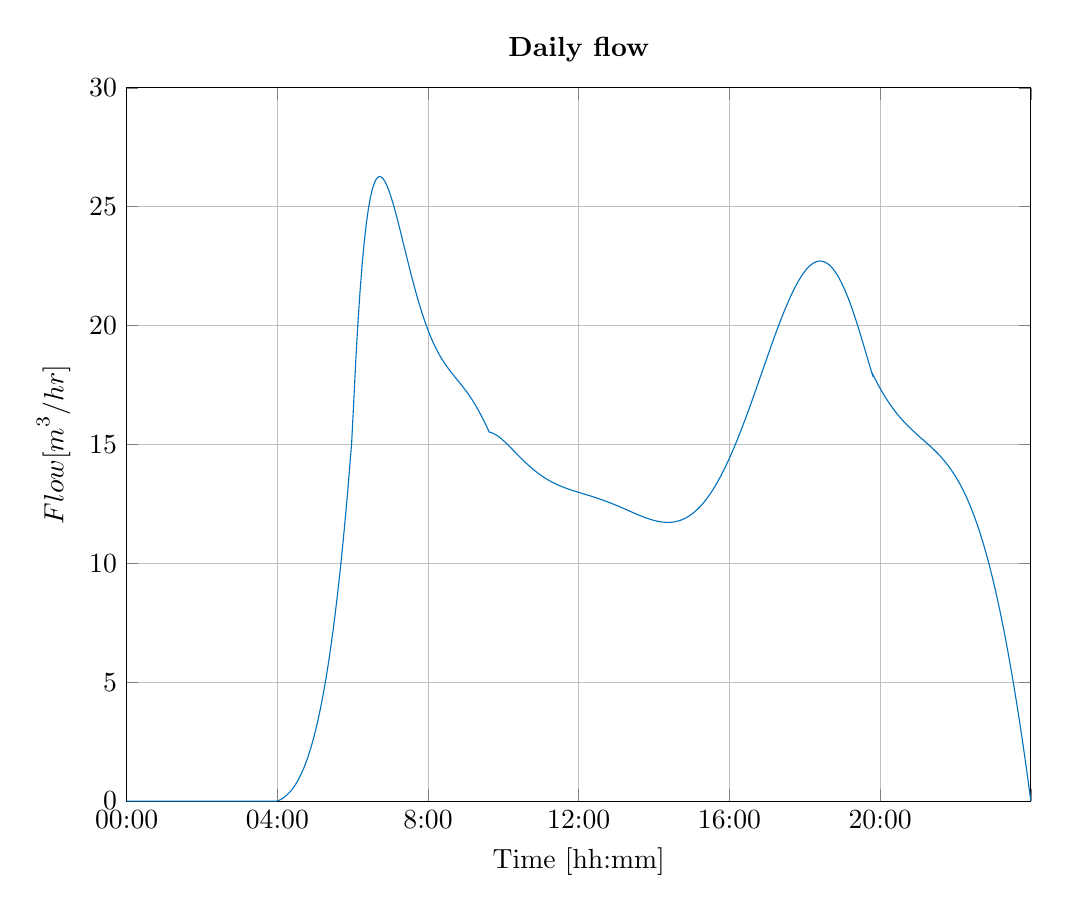
\begin{tikzpicture}

\begin{axis}[%
width=4.521in,
height=3.566in,
at={(0.758in,0.481in)},
scale only axis,
xmin=0,
xmax=24,
xtick={0,4,8,12,16,20,24},
xticklabels={{00:00},{04:00},{8:00},{12:00},{16:00},{20:00}},
xlabel={Time [hh:mm]},
xmajorgrids,
ymin=0,
ymax=30,
ylabel={$\text{Flow [m}^\text{3}\text{/hr]}$},
ymajorgrids,
axis background/.style={fill=white},
title style={font=\bfseries},
title={Daily flow}
]
\addplot [color=mycolor1,solid,forget plot]
  table[row sep=crcr]{%
0.000277777777777778	0\\
0.0558333333333333	0\\
0.111111111111111	0\\
0.166388888888889	0\\
0.221666666666667	0\\
0.276944444444444	0\\
0.332222222222222	0\\
0.3875	0\\
0.442777777777778	0\\
0.498055555555556	0\\
0.553333333333333	0\\
0.608611111111111	0\\
0.663888888888889	0\\
0.719166666666667	0\\
0.774722222222222	0\\
0.83	0\\
0.885277777777778	0\\
0.940555555555556	0\\
0.995833333333333	0\\
1.05111111111111	0\\
1.10638888888889	0\\
1.16166666666667	0\\
1.21694444444444	0\\
1.27222222222222	0\\
1.3275	0\\
1.38277777777778	0\\
1.43805555555556	0\\
1.49361111111111	0\\
1.54888888888889	0\\
1.60416666666667	0\\
1.65944444444444	0\\
1.71472222222222	0\\
1.77	0\\
1.82527777777778	0\\
1.88055555555556	0\\
1.93583333333333	0\\
1.99111111111111	0\\
2.04638888888889	0\\
2.10166666666667	0\\
2.15694444444444	0\\
2.2125	0\\
2.26777777777778	0\\
2.32305555555556	0\\
2.37833333333333	0\\
2.43361111111111	0\\
2.48888888888889	0\\
2.54416666666667	0\\
2.59944444444444	0\\
2.65472222222222	0\\
2.71	0\\
2.76527777777778	0\\
2.82055555555556	0\\
2.87583333333333	0\\
2.93138888888889	0\\
2.98666666666667	0\\
3.04194444444444	0\\
3.09722222222222	0\\
3.1525	0\\
3.20777777777778	0\\
3.26305555555556	0\\
3.31833333333333	0\\
3.37361111111111	0\\
3.42888888888889	0\\
3.48416666666667	0\\
3.53944444444444	0\\
3.59472222222222	0\\
3.65027777777778	0\\
3.70555555555556	0\\
3.76083333333333	0\\
3.81611111111111	0\\
3.87138888888889	0\\
3.92666666666667	0\\
3.98194444444444	0\\
4.03722222222222	0.0253116199877425\\
4.0925	0.0698997844514471\\
4.14777777777778	0.123627484351768\\
4.20305555555556	0.187402299591284\\
4.25833333333333	0.262173247962596\\
4.31361111111111	0.348930848605892\\
4.36916666666667	0.449243195847707\\
4.42444444444444	0.56318529486757\\
4.47972222222222	0.6923402478218\\
4.535	0.837864480246074\\
4.59027777777778	1.0009555298502\\
4.64555555555556	1.18285182754717\\
4.70083333333333	1.38483243145009\\
4.75611111111111	1.60821671383706\\
4.81138888888889	1.85436400108382\\
4.86666666666667	2.12467316656442\\
4.92194444444444	2.42058217651993\\
4.97722222222222	2.74356758889462\\
5.0325	3.09514400514065\\
5.08777777777778	3.47686347499025\\
5.14333333333333	3.89247535584648\\
5.19861111111111	4.33945540280529\\
5.25388888888889	4.82146111600829\\
5.30916666666667	5.3401876171863\\
5.36444444444444	5.89736379043894\\
5.41972222222222	6.49475140457786\\
5.475	7.13414418843844\\
5.53027777777778	7.81736685915861\\
5.58555555555556	8.54627410342655\\
5.64083333333333	9.32274951169527\\
5.69611111111111	10.1487044653658\\
5.75138888888889	11.0260769769383\\
5.80666666666667	11.9568304831307\\
5.86222222222222	12.9480511784066\\
5.9175	13.9918458150724\\
5.97277777777778	15.0950617905803\\
6.02805555555556	16.823793240725\\
6.08333333333333	18.5851901254761\\
6.13861111111111	20.1159971296799\\
6.19388888888889	21.4340601856913\\
6.24916666666667	22.5563795570816\\
6.30444444444444	23.4991288327962\\
6.35972222222222	24.2776739214883\\
6.415	24.9065920456971\\
6.47027777777778	25.3996907361744\\
6.52555555555556	25.7700268260359\\
6.58111111111111	26.0309724854148\\
6.63638888888889	26.1915775909267\\
6.69166666666667	26.2643295004458\\
6.71527777777778	26.2711762322699\\
6.74694444444444	26.2594688566887\\
6.80222222222222	26.1865806715122\\
6.8575	26.0546133200918\\
6.91277777777778	25.8718975352755\\
6.96805555555556	25.6461654017753\\
7.02333333333333	25.3845693503727\\
7.07861111111111	25.093701152245\\
7.13388888888889	24.7796109131781\\
7.18916666666667	24.4478260678383\\
7.24444444444444	24.1033703740255\\
7.3	23.7489976415403\\
7.35527777777778	23.3923409180415\\
7.41055555555556	23.0352696291931\\
7.46583333333333	22.6809806664884\\
7.52111111111111	22.3322623111205\\
7.57638888888889	21.9915132285064\\
7.63166666666667	21.6607614621937\\
7.68694444444444	21.3416834284653\\
7.74222222222222	21.0356229103074\\
7.7975	20.7436100517911\\
7.85277777777778	20.4663803523041\\
7.90805555555556	20.2043936608642\\
7.96333333333333	19.9578531701486\\
8.01888888888889	19.7256015373438\\
8.07416666666667	19.5097065626574\\
8.12944444444445	19.3085146248252\\
8.18472222222222	19.1213913744252\\
8.24	18.9475408724914\\
8.29527777777778	18.7860245848415\\
8.35055555555556	18.6357803762949\\
8.40583333333333	18.4956415049321\\
8.46111111111111	18.3643556163541\\
8.51638888888889	18.2406037379418\\
8.57166666666667	18.1230192730067\\
8.62694444444444	18.0102069952532\\
8.68222222222222	17.9007620427267\\
8.73777777777778	17.7927515016334\\
8.79305555555556	17.6858827014834\\
8.84833333333333	17.5782922900405\\
8.90361111111111	17.4687271872688\\
8.95888888888889	17.3560197443922\\
9.01416666666667	17.2391067380182\\
9.06944444444444	17.1170483646679\\
9.12472222222222	16.989047234521\\
9.18	16.8544673661896\\
9.23527777777778	16.7128531806791\\
9.29055555555555	16.5639484957291\\
9.34583333333333	16.4077155198834\\
9.40111111111111	16.2443538471006\\
9.45666666666667	16.0734492705001\\
9.51194444444444	15.8974459769512\\
9.56722222222222	15.7165329514564\\
9.6225	15.522011721602\\
9.67777777777778	15.5003376203765\\
9.73305555555556	15.4653687718832\\
9.78833333333333	15.4189035249767\\
9.84361111111111	15.3626015245759\\
9.89888888888889	15.2979902951867\\
9.95416666666667	15.226471647195\\
10.0094444444444	15.1493279070675\\
10.0647222222222	15.0677279752757\\
10.12	14.9827332124832\\
10.1752777777778	14.895303156487\\
10.2308333333333	14.8058511966964\\
10.2861111111111	14.716047248561\\
10.3413888888889	14.6261336083568\\
10.3966666666667	14.5367159949384\\
10.4519444444444	14.4483244534955\\
10.5072222222222	14.3614181003605\\
10.5625	14.2763897163188\\
10.6177777777778	14.1935701858514\\
10.6730555555556	14.1132327871275\\
10.7283333333333	14.0355973335303\\
10.7836111111111	13.9608341702333\\
10.8388888888889	13.8890680259374\\
10.8941666666667	13.820381723338\\
10.9497222222222	13.7544982128912\\
11.005	13.69208587487\\
11.0602777777778	13.632785252481\\
11.1155555555556	13.5765457570232\\
11.1708333333333	13.5232914101064\\
11.2261111111111	13.4729237493115\\
11.2813888888889	13.4253246042145\\
11.3366666666667	13.3803587504631\\
11.3919444444444	13.3378764381954\\
11.4472222222222	13.2977158024324\\
11.5025	13.2597051539569\\
11.5577777777778	13.2236651535449\\
11.6130555555556	13.1894108722306\\
11.6686111111111	13.1565933458146\\
11.7238888888889	13.1253495770254\\
11.7791666666667	13.0953211834007\\
11.8344444444444	13.066319282095\\
11.8897222222222	13.0381580699579\\
11.945	13.0106562419601\\
12.0002777777778	12.9836383104518\\
12.0555555555556	12.9569358275542\\
12.1108333333333	12.9303885104412\\
12.1661111111111	12.9038452757326\\
12.2213888888889	12.8771651819999\\
12.2766666666667	12.8502182816276\\
12.3319444444444	12.8228863886609\\
12.3875	12.7949225472487\\
12.4427777777778	12.7665133406187\\
12.4980555555556	12.7374411963445\\
12.5533333333333	12.7076410476748\\
12.6086111111111	12.6770621946195\\
12.6638888888889	12.6456685933607\\
12.7191666666667	12.6134390736618\\
12.7744444444444	12.5803674864141\\
12.8297222222222	12.5464627824837\\
12.885	12.5117490275654\\
12.9402777777778	12.4762653514501\\
12.9955555555556	12.440065836546\\
13.0508333333333	12.4032193472793\\
13.1063888888889	12.3656200483233\\
13.1616666666667	12.3277420659092\\
13.2169444444444	12.2895104352065\\
13.2722222222222	12.2510503924397\\
13.3275	12.2125002817562\\
13.3827777777778	12.1740110711074\\
13.4380555555556	12.1357458263798\\
13.4933333333333	12.0978791368763\\
13.5486111111111	12.0605965079757\\
13.6038888888889	12.0240937098241\\
13.6591666666667	11.9885760917159\\
13.7144444444444	11.9542578629516\\
13.7697222222222	11.9213613405481\\
13.8252777777778	11.8899637226625\\
13.8805555555556	11.8606161502038\\
13.9358333333333	11.8333991562608\\
13.9911111111111	11.8085594259439\\
14.0463888888889	11.7863475825768\\
14.1016666666667	11.7670172871845\\
14.1569444444444	11.7508243218015\\
14.2122222222222	11.7380256569774\\
14.2675	11.7288785058894\\
14.3227777777778	11.7236393703104\\
14.3644444444444	11.722428041888\\
14.3780555555556	11.7225630726145\\
14.4333333333333	11.7259017870532\\
14.4886111111111	11.7339040601805\\
14.5438888888889	11.7468138356072\\
14.5994444444444	11.7649735911212\\
14.6547222222222	11.7884344800392\\
14.71	11.8174983933753\\
14.7652777777778	11.8523810438711\\
14.8205555555556	11.8932886764353\\
14.8758333333333	11.9404171189284\\
14.9311111111111	11.9939508429307\\
14.9863888888889	12.0540620433162\\
15.0416666666667	12.1209097303273\\
15.0969444444444	12.1946388411309\\
15.1522222222222	12.2753793732638\\
15.2075	12.3632455412137\\
15.2627777777778	12.458334954429\\
15.3183333333333	12.5612609184825\\
15.3736111111111	12.6710564397917\\
15.4288888888889	12.7882608034172\\
15.4841666666667	12.9128974783746\\
15.5394444444444	13.0449696777814\\
15.5947222222222	13.1844597308445\\
15.65	13.3313284957325\\
15.7052777777778	13.4855148179045\\
15.7605555555556	13.6469350289457\\
15.8158333333333	13.8154824889917\\
15.8711111111111	13.9910271850016\\
15.9263888888889	14.1734153727009\\
15.9816666666667	14.3624692703956\\
16.0372222222222	14.5589852627889\\
16.0925	14.7607706344896\\
16.1477777777778	14.9685406277427\\
16.2030555555556	15.182019276075\\
16.2583333333333	15.4009059177912\\
16.3136111111111	15.62487524787\\
16.3688888888889	15.8535774423497\\
16.4241666666667	16.0866383467854\\
16.4794444444444	16.3236597394137\\
16.5347222222222	16.56421966529\\
16.59	16.8078728503001\\
16.6452777777778	17.0541511855497\\
16.7005555555556	17.3025642976623\\
16.7561111111111	17.5538598685704\\
16.8113888888889	17.804989790489\\
16.8666666666667	18.0566538784781\\
16.9219444444444	18.3082799573848\\
16.9772222222222	18.5592777051533\\
17.0325	18.8090397398467\\
17.0877777777778	19.0569428094604\\
17.1430555555556	19.302349070703\\
17.1983333333333	19.5446074728955\\
17.2536111111111	19.78305523817\\
17.3088888888889	20.0170194463285\\
17.3641666666667	20.2458187233053\\
17.4194444444444	20.4687650417304\\
17.475	20.6862353594024\\
17.5302777777778	20.8953565443601\\
17.5855555555556	21.0965368709193\\
17.6408333333333	21.2890818852858\\
17.6961111111111	21.4723011538097\\
17.7513888888889	21.6455107471918\\
17.8066666666667	21.8080358487508\\
17.8619444444444	21.9592134810133\\
17.9172222222222	22.0983953663221\\
17.9725	22.2249509079598\\
18.0277777777778	22.3382703071028\\
18.0830555555556	22.4377678075961\\
18.1383333333333	22.5228850799685\\
18.1938888888889	22.5934090608999\\
18.2491666666667	22.6481397531112\\
18.3044444444444	22.687013484547\\
18.3597222222222	22.7096184332852\\
18.4069444444444	22.7157672115064\\
18.415	22.7155892261752\\
18.4702777777778	22.7046111659752\\
18.5255555555556	22.6764246270588\\
18.5808333333333	22.6308295774281\\
18.6361111111111	22.5676902703252\\
18.6913888888889	22.4869400945647\\
18.7466666666667	22.3885865665959\\
18.8019444444444	22.2727164962207\\
18.8572222222222	22.1395013113591\\
18.9127777777778	21.9884046907302\\
18.9680555555556	21.8212966375205\\
19.0233333333333	21.6379237200741\\
19.0786111111111	21.438852927126\\
19.1338888888889	21.2247650125493\\
19.1891666666667	20.9964608394426\\
19.2444444444444	20.7548678870517\\
19.2997222222222	20.5010469578642\\
19.355	20.2361990421275\\
19.4102777777778	19.9616723866532\\
19.4655555555556	19.6789697349512\\
19.5208333333333	19.3897557568775\\
19.5761111111111	19.0958646716369\\
19.6313888888889	18.7993080646822\\
19.6869444444444	18.5007930664555\\
19.7422222222222	18.2057058664098\\
19.7944444444444	17.9310429893127\\
19.7975	17.9712077467308\\
19.8527777777778	17.7945965721496\\
19.9080555555556	17.6245352460121\\
19.9633333333333	17.4610087993307\\
20.0186111111111	17.3039706077282\\
20.0738888888889	17.1533433910085\\
20.1291666666667	17.009020212564\\
20.1844444444444	16.8708654786759\\
20.2397222222222	16.7387159388962\\
20.295	16.6123816848603\\
20.3502777777778	16.4916471500202\\
20.4058333333333	16.3757054334303\\
20.4611111111111	16.2654509042094\\
20.5163888888889	16.1600039465212\\
20.5716666666667	16.059056251153\\
20.6269444444444	15.962278852998\\
20.6822222222222	15.8693231315995\\
20.7375	15.7798218107216\\
20.7927777777778	15.6933899569454\\
20.8480555555556	15.60962598043\\
20.9033333333333	15.5281126336167\\
20.9586111111111	15.4484180110166\\
21.0138888888889	15.3700965492671\\
21.0691666666667	15.2926900256208\\
21.1247222222222	15.215342134617\\
21.18	15.138343775053\\
21.2352777777778	15.0608172434315\\
21.2905555555556	14.9822636379372\\
21.3458333333333	14.9021763995504\\
21.4011111111111	14.8200423135123\\
21.4563888888889	14.7353425085163\\
21.5116666666667	14.6475534555746\\
21.5669444444444	14.5561479682926\\
21.6222222222222	14.4605962025472\\
21.6775	14.3603666550289\\
21.7327777777778	14.2549271642739\\
21.7880555555556	14.1437459087728\\
21.8436111111111	14.0256854580975\\
21.8988888888889	13.9013960690233\\
21.9541666666667	13.7697788644188\\
22.0094444444444	13.6303134055713\\
22.0647222222222	13.482484597365\\
22.12	13.3257836874186\\
22.1752777777778	13.1597092666837\\
22.2305555555556	12.9837682677166\\
22.2858333333333	12.7974769650064\\
22.3411111111111	12.6003619743286\\
22.3963888888889	12.3919612525865\\
22.4516666666667	12.171825096732\\
22.5069444444444	11.9395171440934\\
22.5625	11.6933522142751\\
22.6177777777778	11.4353836081672\\
22.6730555555556	11.1640222339559\\
22.7283333333333	10.8788951740098\\
22.7836111111111	10.5796478535801\\
22.8388888888889	10.2659450406956\\
22.8941666666667	9.93747184519214\\
22.9494444444444	9.59393471839094\\
23.0047222222222	9.23506245283158\\
23.06	8.86060718151758\\
23.1152777777778	8.47034537802801\\
23.1705555555556	8.06407885554673\\
23.2258333333333	7.64163576702804\\
23.2813888888889	7.20062533673316\\
23.3366666666667	6.7453410852948\\
23.3919444444444	6.27353239724316\\
23.4472222222222	5.78514293265396\\
23.5025	5.28014769544862\\
23.5577777777778	4.75855402960957\\
23.6130555555556	4.22040262243047\\
23.6683333333333	3.66576849981149\\
23.7236111111111	3.09476203037543\\
23.7788888888889	2.50752992124998\\
23.8341666666667	1.90425622028985\\
23.8894444444444	1.28516331359072\\
23.9447222222222	0.650512926466693\\
24	0.000607122804183746\\
};
\end{axis}
\end{tikzpicture}%
\caption{A daily flow profile for zone 8 and 9.}
\label{fig:APP_flow_profile_zone8_9}
\end{figure} 

\begin{figure}[H]
\centering
% This file was created by matlab2tikz.
%
%The latest updates can be retrieved from
%  http://www.mathworks.com/matlabcentral/fileexchange/22022-matlab2tikz-matlab2tikz
%where you can also make suggestions and rate matlab2tikz.
%
\definecolor{mycolor1}{rgb}{0.00000,0.44700,0.74100}%
%
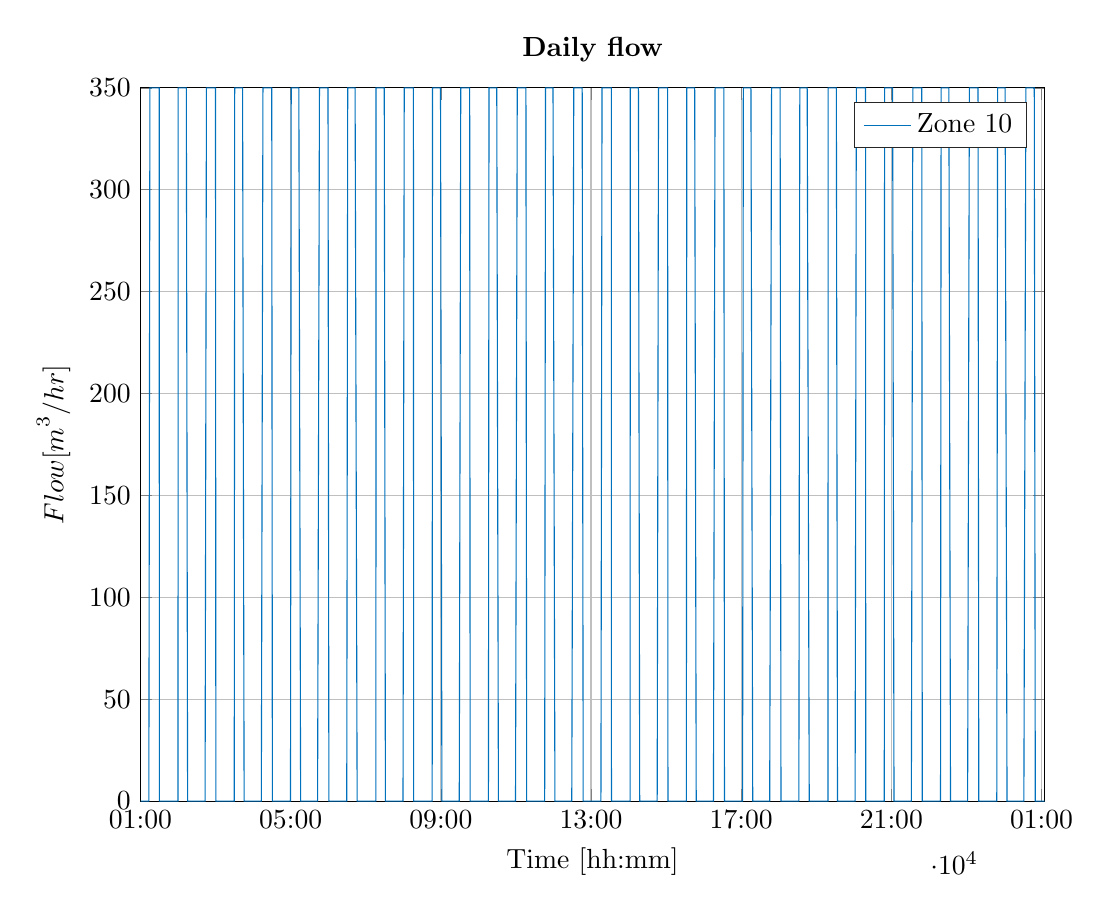
\begin{tikzpicture}

\begin{axis}[%
width=4.521in,
height=3.566in,
at={(0.758in,0.481in)},
scale only axis,
xmin=3600,
xmax=90000,
xtick={3600,17950,32300,46650,61000,75350,89700},
xticklabels={{01:00},{05:00},{09:00},{13:00},{17:00},{21:00},{01:00},{},{},{}},
xlabel={Time [hh:mm]},
xmajorgrids,
ymin=0,
ymax=350,
ylabel={$\text{Flow [m}^\text{3}\text{/hr]}$},
ymajorgrids,
axis background/.style={fill=white},
title style={font=\bfseries},
title={Daily flow},
legend style={legend cell align=left,align=left,draw=white!15!black}
]
\addplot [color=mycolor1,solid]
  table[row sep=crcr]{%
3599	0\\
3799	0\\
3998	0\\
4197	0\\
4396	0\\
4501	350\\
4595	350\\
4794	350\\
4993	350\\
5192	350\\
5391	350\\
5401	0\\
5590	0\\
5789	0\\
5988	0\\
6188	0\\
6387	0\\
6586	0\\
6785	0\\
6984	0\\
7183	0\\
7201	350\\
7382	350\\
7581	350\\
7780	350\\
7979	350\\
8101	0\\
8178	0\\
8377	0\\
8577	0\\
8776	0\\
8975	0\\
9174	0\\
9373	0\\
9572	0\\
9771	0\\
9901	350\\
9970	350\\
10169	350\\
10368	350\\
10567	350\\
10766	350\\
10801	0\\
10965	0\\
11165	0\\
11364	0\\
11563	0\\
11762	0\\
11961	0\\
12160	0\\
12359	0\\
12558	0\\
12601	350\\
12757	350\\
12956	350\\
13155	350\\
13354	350\\
13501	0\\
13554	0\\
13753	0\\
13952	0\\
14151	0\\
14350	0\\
14549	0\\
14748	0\\
14947	0\\
15146	0\\
15301	350\\
15345	350\\
15544	350\\
15743	350\\
15942	350\\
16142	350\\
16201	0\\
16341	0\\
16540	0\\
16739	0\\
16938	0\\
17137	0\\
17336	0\\
17535	0\\
17734	0\\
17933	0\\
18001	350\\
18132	350\\
18331	350\\
18531	350\\
18730	350\\
18901	0\\
18929	0\\
19128	0\\
19327	0\\
19526	0\\
19725	0\\
19924	0\\
20123	0\\
20322	0\\
20521	0\\
20701	350\\
20720	350\\
20920	350\\
21119	350\\
21318	350\\
21517	350\\
21601	0\\
21716	0\\
21915	0\\
22114	0\\
22313	0\\
22512	0\\
22711	0\\
22910	0\\
23109	0\\
23308	0\\
23401	350\\
23508	350\\
23707	350\\
23906	350\\
24105	350\\
24301	0\\
24304	0\\
24503	0\\
24702	0\\
24901	0\\
25100	0\\
25299	0\\
25498	0\\
25697	0\\
25897	0\\
26096	0\\
26101	350\\
26295	350\\
26494	350\\
26693	350\\
26892	350\\
27001	0\\
27091	0\\
27290	0\\
27489	0\\
27688	0\\
27887	0\\
28086	0\\
28285	0\\
28485	0\\
28684	0\\
28801	350\\
28883	350\\
29082	350\\
29281	350\\
29480	350\\
29679	350\\
29701	0\\
29878	0\\
30077	0\\
30276	0\\
30475	0\\
30674	0\\
30874	0\\
31073	0\\
31272	0\\
31471	0\\
31501	350\\
31670	350\\
31869	350\\
32068	350\\
32267	350\\
32401	0\\
32466	0\\
32665	0\\
32864	0\\
33063	0\\
33263	0\\
33462	0\\
33661	0\\
33860	0\\
34059	0\\
34201	350\\
34258	350\\
34457	350\\
34656	350\\
34855	350\\
35054	350\\
35101	0\\
35253	0\\
35452	0\\
35651	0\\
35851	0\\
36050	0\\
36249	0\\
36448	0\\
36647	0\\
36846	0\\
36901	350\\
37045	350\\
37244	350\\
37443	350\\
37642	350\\
37801	0\\
37841	0\\
38040	0\\
38240	0\\
38439	0\\
38638	0\\
38837	0\\
39036	0\\
39235	0\\
39434	0\\
39601	350\\
39633	350\\
39832	350\\
40031	350\\
40230	350\\
40429	350\\
40501	0\\
40628	0\\
40828	0\\
41027	0\\
41226	0\\
41425	0\\
41624	0\\
41823	0\\
42022	0\\
42221	0\\
42301	350\\
42420	350\\
42619	350\\
42818	350\\
43017	350\\
43201	0\\
43217	0\\
43416	0\\
43615	0\\
43814	0\\
44013	0\\
44212	0\\
44411	0\\
44610	0\\
44809	0\\
45001	350\\
45008	350\\
45207	350\\
45406	350\\
45606	350\\
45805	350\\
45901	0\\
46004	0\\
46203	0\\
46402	0\\
46601	0\\
46800	0\\
46999	0\\
47198	0\\
47397	0\\
47596	0\\
47701	350\\
47795	350\\
47994	350\\
48194	350\\
48393	350\\
48592	350\\
48601	0\\
48791	0\\
48990	0\\
49189	0\\
49388	0\\
49587	0\\
49786	0\\
49985	0\\
50184	0\\
50383	0\\
50401	350\\
50583	350\\
50782	350\\
50981	350\\
51180	350\\
51301	0\\
51379	0\\
51578	0\\
51777	0\\
51976	0\\
52175	0\\
52374	0\\
52573	0\\
52772	0\\
52971	0\\
53101	350\\
53171	350\\
53370	350\\
53569	350\\
53768	350\\
53967	350\\
54001	0\\
54166	0\\
54365	0\\
54564	0\\
54763	0\\
54962	0\\
55161	0\\
55360	0\\
55560	0\\
55759	0\\
55801	350\\
55958	350\\
56157	350\\
56356	350\\
56555	350\\
56701	0\\
56754	0\\
56953	0\\
57152	0\\
57351	0\\
57550	0\\
57749	0\\
57949	0\\
58148	0\\
58347	0\\
58501	350\\
58546	350\\
58745	350\\
58944	350\\
59143	350\\
59342	350\\
59401	0\\
59541	0\\
59740	0\\
59939	0\\
60138	0\\
60337	0\\
60537	0\\
60736	0\\
60935	0\\
61134	0\\
61201	350\\
61333	350\\
61532	350\\
61731	350\\
61930	350\\
62101	0\\
62129	0\\
62328	0\\
62527	0\\
62726	0\\
62926	0\\
63125	0\\
63324	0\\
63523	0\\
63722	0\\
63901	350\\
63921	350\\
64120	350\\
64319	350\\
64518	350\\
64717	350\\
64801	0\\
64916	0\\
65115	0\\
65314	0\\
65514	0\\
65713	0\\
65912	0\\
66111	0\\
66310	0\\
66509	0\\
66601	350\\
66708	350\\
66907	350\\
67106	350\\
67305	350\\
67501	0\\
67504	0\\
67703	0\\
67903	0\\
68102	0\\
68301	0\\
68500	0\\
68699	0\\
68898	0\\
69097	0\\
69296	0\\
69301	350\\
69495	350\\
69694	350\\
69893	350\\
70092	350\\
70201	0\\
70292	0\\
70491	0\\
70690	0\\
70889	0\\
71088	0\\
71287	0\\
71486	0\\
71685	0\\
71884	0\\
72001	350\\
72083	350\\
72282	350\\
72481	350\\
72680	350\\
72880	350\\
72901	0\\
73079	0\\
73278	0\\
73477	0\\
73676	0\\
73875	0\\
74074	0\\
74273	0\\
74472	0\\
74671	0\\
74701	350\\
74870	350\\
75069	350\\
75269	350\\
75468	350\\
75601	0\\
75667	0\\
75866	0\\
76065	0\\
76264	0\\
76463	0\\
76662	0\\
76861	0\\
77060	0\\
77259	0\\
77401	350\\
77458	350\\
77657	350\\
77857	350\\
78056	350\\
78255	350\\
78301	0\\
78454	0\\
78653	0\\
78852	0\\
79051	0\\
79250	0\\
79449	0\\
79648	0\\
79847	0\\
80046	0\\
80101	350\\
80246	350\\
80445	350\\
80644	350\\
80843	350\\
81001	0\\
81042	0\\
81241	0\\
81440	0\\
81639	0\\
81838	0\\
82037	0\\
82236	0\\
82435	0\\
82635	0\\
82801	350\\
82834	350\\
83033	350\\
83232	350\\
83431	350\\
83630	350\\
83701	0\\
83829	0\\
84028	0\\
84227	0\\
84426	0\\
84625	0\\
84824	0\\
85023	0\\
85223	0\\
85422	0\\
85501	350\\
85621	350\\
85820	350\\
86019	350\\
86218	350\\
86401	0\\
86417	0\\
86616	0\\
86815	0\\
87014	0\\
87213	0\\
87412	0\\
87612	0\\
87811	0\\
88010	0\\
88201	350\\
88209	350\\
88408	350\\
88607	350\\
88806	350\\
89005	350\\
89101	0\\
89204	0\\
89403	0\\
89602	0\\
90000	0\\
};
\addlegendentry{Zone 10};

\end{axis}
\end{tikzpicture}%
\caption{A daily flow profile for zone 10.}
\label{fig:APP_flow_profile_zone10}
\end{figure} 

From zone ten a pump is pumping the wastewater to the main sewer line every 30 minuted for a period of 15 minutes. The pump has a pumping capacity of 0,350 $m^3/s$ which have been state by Fredericia and seen in tabel \ref{tab:pump_info}. Therefore the flow profile for this area will be a constant input of 0,350 $m^3/s$ for 15 minutes every 30 minute. 

\begin{figure}[H]
\centering
% This file was created by matlab2tikz.
%
%The latest updates can be retrieved from
%  http://www.mathworks.com/matlabcentral/fileexchange/22022-matlab2tikz-matlab2tikz
%where you can also make suggestions and rate matlab2tikz.
%
\definecolor{mycolor1}{rgb}{0.00000,0.44700,0.74100}%
%
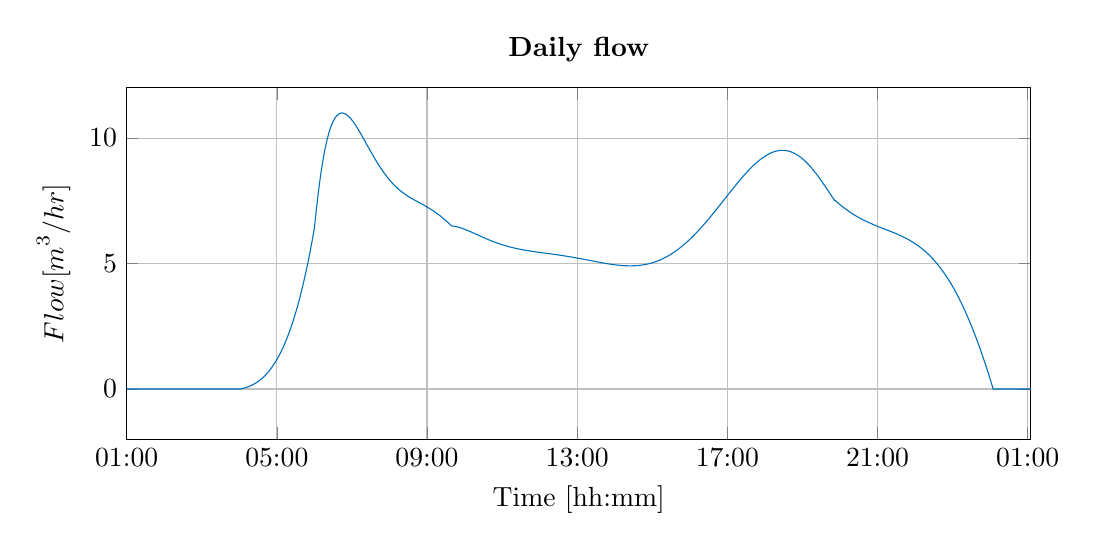
\begin{tikzpicture}

\begin{axis}[%
width=4.521in,
height=1.7566in,
at={(0.758in,0.481in)},
scale only axis,
xmin=3600,
xmax=90000,
xtick={3600,17950,32300,46650,61000,75350,89700},
xticklabels={{01:00},{05:00},{09:00},{13:00},{17:00},{21:00},{01:00},{},{},{}},
xlabel={Time [hh:mm]},
xmajorgrids,
ymin=-2,
scaled x ticks = false,
ymax=12,
ylabel={$\text{Flow [m}^\text{3}\text{/hr]}$},
ymajorgrids,
axis background/.style={fill=white},
title style={font=\bfseries},
title={Daily flow},
legend style={legend cell align=left,align=left,draw=white!15!black}
]
\addplot [color=mycolor1,solid]
  table[row sep=crcr]{%
3599	0\\
3799	0\\
3998	0\\
4197	0\\
4396	0\\
4595	0\\
4794	0\\
4993	0\\
5192	0\\
5391	0\\
5590	0\\
5789	0\\
5988	0\\
6188	0\\
6387	0\\
6586	0\\
6785	0\\
6984	0\\
7183	0\\
7382	0\\
7581	0\\
7780	0\\
7979	0\\
8178	0\\
8377	0\\
8577	0\\
8776	0\\
8975	0\\
9174	0\\
9373	0\\
9572	0\\
9771	0\\
9970	0\\
10169	0\\
10368	0\\
10567	0\\
10766	0\\
10965	0\\
11165	0\\
11364	0\\
11563	0\\
11762	0\\
11961	0\\
12160	0\\
12359	0\\
12558	0\\
12757	0\\
12956	0\\
13155	0\\
13354	0\\
13554	0\\
13753	0\\
13952	0\\
14151	0\\
14350	0\\
14549	0.0118795817392918\\
14748	0.0308234886727714\\
14947	0.0536220064953477\\
15146	0.0806564302629574\\
15345	0.112325407078907\\
15544	0.149044961178419\\
15743	0.191248499321518\\
15942	0.239386796494379\\
16142	0.294219018527653\\
16341	0.355684311119568\\
16540	0.424543027612383\\
16739	0.501314964811748\\
16938	0.586536920266521\\
17137	0.680762559721937\\
17336	0.784562264880996\\
17535	0.898522961474619\\
17734	1.02324792763982\\
17933	1.15935658260669\\
18132	1.30748425569367\\
18331	1.46828193561114\\
18531	1.64332586637081\\
18730	1.83154997948346\\
18929	2.03449175519504\\
19128	2.25286199078694\\
19327	2.48738559227373\\
19526	2.73880120545836\\
19725	3.00786082729631\\
19924	3.29532939756776\\
20123	3.60198437085838\\
20322	3.92861526884855\\
20521	4.27602321291099\\
20720	4.64502043701694\\
20920	5.03845465852228\\
21119	5.45322797024621\\
21318	5.89209302976077\\
21517	6.35590130026059\\
21716	7.10296901560315\\
21915	7.83289111533979\\
22114	8.46684476614284\\
22313	9.01227479884609\\
22512	9.47627257617931\\
22711	9.86558394536148\\
22910	10.1866171906544\\
23109	10.4454509859616\\
23308	10.6478423474075\\
23508	10.7998753654395\\
23707	10.9051880464705\\
23906	10.9695025028465\\
24105	10.9973672088713\\
24175	10.9993066025719\\
24304	10.9930487839045\\
24503	10.9605399449714\\
24702	10.9035674592995\\
24901	10.8256000969293\\
25100	10.7298565832501\\
25299	10.6193135516508\\
25498	10.4967134960161\\
25697	10.3645727233541\\
25897	10.2244742079456\\
26096	10.0799149610652\\
26295	9.93209529980857\\
26494	9.7827053527254\\
26693	9.6332488643236\\
26892	9.48505114765667\\
27091	9.33926703689998\\
27290	9.19688883990723\\
27489	9.05875429083206\\
27688	8.92555450267593\\
27887	8.79784191987574\\
28086	8.67603827084613\\
28285	8.56044252061799\\
28485	8.45070637554046\\
28684	8.34800456145935\\
28883	8.25175014165034\\
29082	8.16183011628386\\
29281	8.07804852498982\\
29480	8.00013439941689\\
29679	7.92774971580873\\
29878	7.86049734757461\\
30077	7.79792901788265\\
30276	7.73955325223045\\
30475	7.68484333103265\\
30674	7.63324524213489\\
30874	7.58394452892605\\
31073	7.53684699330472\\
31272	7.49111207349925\\
31471	7.4461561559022\\
31670	7.40140813724263\\
31869	7.35631737717369\\
32068	7.31036165086023\\
32267	7.2630551015267\\
32466	7.21395619301645\\
32665	7.16267566245863\\
32864	7.10888447275947\\
33063	7.05232176521251\\
33263	6.99249604961948\\
33462	6.92990474326307\\
33661	6.86424814160538\\
33860	6.79561814779798\\
34059	6.7242146462003\\
34258	6.65035345505218\\
34457	6.57447427891987\\
34656	6.49833713668959\\
34855	6.4888153972397\\
35054	6.47378620789247\\
35253	6.45399803250556\\
35452	6.430141472223\\
35651	6.40285201621118\\
35851	6.37255498865431\\
36050	6.34008869544113\\
36249	6.3057940293976\\
36448	6.2701118493111\\
36647	6.23344057203945\\
36846	6.1961384905259\\
37045	6.15852602313973\\
37244	6.12088789492031\\
37443	6.08347525161941\\
37642	6.04650770724432\\
37841	6.01017532674433\\
38040	5.9746405435234\\
38240	5.93986870048465\\
38439	5.90632060103044\\
38638	5.87391023942384\\
38837	5.84270734198412\\
39036	5.8127626631628\\
39235	5.78410953454619\\
39434	5.75676535533393\\
39633	5.73073302521139\\
39832	5.70600232097511\\
40031	5.68255121690019\\
40230	5.66034715102461\\
40429	5.63934823677265\\
40628	5.61950442207006\\
40828	5.60066706403399\\
41027	5.58296114379309\\
41226	5.56622163123193\\
41425	5.55037635222371\\
41624	5.53535000103584\\
41823	5.5210649988729\\
42022	5.50744230600601\\
42221	5.49440218776061\\
42420	5.48186493498562\\
42619	5.46975154122447\\
42818	5.45798433542106\\
43017	5.44648757308358\\
43217	5.43513158146358\\
43416	5.42395934944996\\
43615	5.412846849108\\
43814	5.40173115153327\\
44013	5.3905536040869\\
44212	5.37926018460897\\
44411	5.36780181947079\\
44610	5.35613466608918\\
44809	5.34422036126217\\
45008	5.33202623563196\\
45207	5.31952549521548\\
45406	5.30669737156585\\
45606	5.29346017819263\\
45805	5.27993787640668\\
46004	5.26606308218105\\
46203	5.25184005225066\\
46402	5.23727937051237\\
46601	5.22239792539026\\
46800	5.20721886092982\\
46999	5.19177150333153\\
47198	5.17609126368296\\
47397	5.16021951725179\\
47596	5.14420346093724\\
47795	5.1280959494349\\
47994	5.11195531099861\\
48194	5.09576437814526\\
48393	5.07975400522986\\
48592	5.06391658002326\\
48791	5.04833012650349\\
48990	5.03307694354333\\
49189	5.01824331699232\\
49388	5.00391921750719\\
49587	4.99019798457275\\
49786	4.97717599782331\\
49985	4.96495233778306\\
50184	4.95362843509666\\
50383	4.943307710119\\
50583	4.93405188689422\\
50782	4.92606025598407\\
50981	4.91939081037052\\
51180	4.91415116238873\\
51379	4.91044899364868\\
51578	4.90839165591487\\
51712	4.9079865712648\\
51777	4.90808576487176\\
51976	4.90963679453481\\
52175	4.91314866779855\\
52374	4.91872334657675\\
52573	4.92646042182932\\
52772	4.93645670446153\\
52971	4.94880581752605\\
53171	4.96367843878419\\
53370	4.98101222824093\\
53569	5.00095695851902\\
53768	5.0235894659558\\
53967	5.04898141570374\\
54166	5.07719892245806\\
54365	5.1083021797488\\
54564	5.14234509685707\\
54763	5.17937494682204\\
54962	5.2194320240094\\
55161	5.26254931252127\\
55360	5.3087521683705\\
55560	5.35831363652653\\
55759	5.41074731626227\\
55958	5.46629385879316\\
56157	5.5249451513103\\
56356	5.58668407368437\\
56555	5.65148427078218\\
56754	5.71930994507271\\
56953	5.79011566840136\\
57152	5.86384621208262\\
57351	5.94043640113411\\
57550	6.01981098776936\\
57749	6.10188454891874\\
57949	6.18699331933262\\
58148	6.27417975568391\\
58347	6.36374657234448\\
58546	6.45556705634981\\
58745	6.54950418071004\\
58944	6.64541065706556\\
59143	6.74312901851093\\
59342	6.84249173198655\\
59541	6.94332133998895\\
59740	7.04543063664093\\
59939	7.14862287411116\\
60138	7.25269200342766\\
60337	7.35742294833695\\
60537	7.46312112327383\\
60736	7.5684963917265\\
60935	7.67383614962592\\
61134	7.77889264659146\\
61333	7.88341102952007\\
61532	7.98712984110427\\
61731	8.08978156040206\\
61930	8.19109318533432\\
62129	8.29078685482113\\
62328	8.38858051695783\\
62527	8.48418863990012\\
62726	8.57732296753143\\
62926	8.66813997197572\\
63125	8.75543900905899\\
63324	8.83938992393095\\
63523	8.91970205878648\\
63722	8.99608652033954\\
63921	9.06825722416748\\
64120	9.13593199128067\\
64319	9.19883369466275\\
64518	9.25669145856857\\
64717	9.30924191419349\\
64916	9.35623050704678\\
65115	9.39741286094565\\
65314	9.43255619917375\\
65514	9.46156981346488\\
65713	9.48395766023341\\
65912	9.4996919189945\\
66111	9.50860166582624\\
66265	9.51071570084851\\
66310	9.51053556425147\\
66509	9.50536364213913\\
66708	9.49297913292957\\
66907	9.47330037663013\\
67106	9.44627279118421\\
67305	9.41187090349721\\
67504	9.37010044906882\\
67703	9.32100053993716\\
67903	9.26434456063948\\
68102	9.20081227631483\\
68301	9.13029168268548\\
68500	9.05297864660904\\
68699	8.9691142905395\\
68898	8.87898757931475\\
69097	8.7829379799462\\
69296	8.68135819828457\\
69495	8.57469698417882\\
69694	8.46346202067126\\
69893	8.34822288367939\\
70092	8.22961408120522\\
70292	8.10772328622543\\
70491	7.98454664202218\\
70690	7.86032948610619\\
70889	7.73599843250721\\
71088	7.61256143877008\\
71260	7.50743087403459\\
71287	7.51820063907476\\
71486	7.44447686225493\\
71685	7.37349539461166\\
71884	7.30524888764713\\
72083	7.23971677314864\\
72282	7.17686568132963\\
72481	7.1166498594239\\
72680	7.05901159030249\\
72880	7.00361077830367\\
73079	6.95092067663724\\
73278	6.90056689002065\\
73477	6.85244797768144\\
73676	6.80645262895079\\
73875	6.76246008188042\\
74074	6.72034054156487\\
74273	6.67995559869046\\
74472	6.64115864831068\\
74671	6.60379530782871\\
74870	6.56770383602209\\
75069	6.53271555120645\\
75269	6.49848613235421\\
75468	6.46517579217891\\
75667	6.43242418353294\\
75866	6.40003902290639\\
76065	6.3678231811337\\
76264	6.33557510171602\\
76463	6.30308921950603\\
76662	6.27015637891697\\
76861	6.23656425276611\\
77060	6.20209776068766\\
77259	6.16653948738713\\
77458	6.12967010150745\\
77657	6.09126877399659\\
77857	6.05090700721646\\
78056	6.00876491594508\\
78255	5.96442247452863\\
78454	5.91765704973439\\
78653	5.86824660546362\\
78852	5.8159701206887\\
79051	5.76060800854582\\
79250	5.70194253427214\\
79449	5.63975823416245\\
79648	5.57384233393689\\
79847	5.50398516697258\\
80046	5.42998059321505\\
80246	5.3512213585326\\
80445	5.26829640596763\\
80644	5.18063001216999\\
80843	5.08803435503968\\
81042	4.99032723314903\\
81241	4.88733248454082\\
81440	4.77888040541312\\
81639	4.66480816839628\\
81838	4.54496024114717\\
82037	4.41918880473945\\
82236	4.28735417230308\\
82435	4.14932520761857\\
82635	4.00423824438883\\
82834	3.85343092398334\\
83033	3.69609085829208\\
83232	3.5321253502789\\
83431	3.36145234825117\\
83630	3.18400086404616\\
83829	2.99971139153463\\
84028	2.80853632539629\\
84227	2.61044037941947\\
84426	2.40540100459686\\
84625	2.19340880871666\\
84824	1.97446797359732\\
85023	1.7485966745654\\
85223	1.51464045938017\\
85422	1.27498654396602\\
85621	1.02854518802803\\
85820	0.775394804106138\\
86019	0.5156298925109\\
86218	0.249361459691136\\
86401	0\\
86417	0\\
86616	0\\
86815	0\\
87014	0\\
87213	0\\
87412	0\\
87612	0\\
87811	0\\
88010	0\\
88209	0\\
88408	0\\
88607	0\\
88806	0\\
89005	0\\
89204	0\\
89403	0\\
89602	0\\
90000	0\\
};

\end{axis}
\end{tikzpicture}%
\caption{A daily flow profile for zone 11.}
\label{fig:APP_flow_profile_zone11}
\end{figure} 


\begin{figure}[H]
	\centering
	\includegraphics[width=0.95\textheight, angle=-90]{report/appendix/figures/Carlsberg_data.png}
	\caption{Daily flow from a brewery and bottling plant in Fredericia.}
	\label{fig:Carlsberg_data}
\end{figure}

\begin{figure}[H]
	\centering
	\includegraphics[width=0.95\textheight, angle=-90]{report/appendix/figures/COD_data.png}
	\caption{COD inflow to the WWTP.}
	\label{fig:COD_data}
\end{figure}

\begin{figure}[H]
	\centering
	\includegraphics[width=0.95\textheight, angle=-90]{report/appendix/figures/Forfos_data.png}
	\caption{Phosphorus inflow to the WWTP.}
	\label{fig:Forfos_data}
\end{figure}

\begin{figure}[H]
	\centering
	\includegraphics[width=0.95\textheight, angle=-90]{report/appendix/figures/kvaelstof_data.png}
	\caption{Nitrogen inflow to the WWTP.}
	\label{fig:kvaelstof_data}
\end{figure}